
\documentclass[a4paper,11pt]{article}
\usepackage[a4paper, margin=8em]{geometry}

% usa i pacchetti per la scrittura in italiano
\usepackage[french,italian]{babel}
\usepackage[T1]{fontenc}
\usepackage[utf8]{inputenc}
\frenchspacing 

% usa i pacchetti per la formattazione matematica
\usepackage{amsmath, amssymb, amsthm, amsfonts}

% usa altri pacchetti
\usepackage{gensymb}
\usepackage{hyperref}
\usepackage{standalone}

% cose fluttuanti
\usepackage{float}

% imposta il titolo
\title{Appunti Calcolo Numerico}
\author{Luca Seggiani}
\date{2025}

% disegni
\usepackage{pgfplots}
\pgfplotsset{width=10cm,compat=1.9}

% imposta lo stile
% usa helvetica
\usepackage[scaled]{helvet}
% usa palatino
\usepackage{palatino}
% usa un font monospazio guardabile
\usepackage{lmodern}

% tikz in sans
\tikzset{every picture/.style={/utils/exec={\sffamily}}}

\renewcommand{\rmdefault}{ppl}
\renewcommand{\sfdefault}{phv}
\renewcommand{\ttdefault}{lmtt}

% circuiti
\usepackage{circuitikz}
\usetikzlibrary{babel}

% disponi il titolo
\makeatletter
\renewcommand{\maketitle} {
	\begin{center} 
		\begin{minipage}[t]{.8\textwidth}
			\textsf{\huge\bfseries \@title} 
		\end{minipage}%
		\begin{minipage}[t]{.2\textwidth}
			\raggedleft \vspace{-1.65em}
			\textsf{\small \@author} \vfill
			\textsf{\small \@date}
		\end{minipage}
		\par
	\end{center}

	\thispagestyle{empty}
	\pagestyle{fancy}
}
\makeatother

% disponi teoremi
\usepackage{tcolorbox}
\newtcolorbox[auto counter, number within=section]{theorem}[2][]{%
	colback=blue!10, 
	colframe=blue!40!black, 
	sharp corners=northwest,
	fonttitle=\sffamily\bfseries, 
	title=Teorema~\thetcbcounter: #2, 
	#1
}

% disponi definizioni
\newtcolorbox[auto counter, number within=section]{definition}[2][]{%
	colback=red!10,
	colframe=red!40!black,
	sharp corners=northwest,
	fonttitle=\sffamily\bfseries,
	title=Definizione~\thetcbcounter: #2,
	#1
}

% disponi problemi
\newtcolorbox[auto counter, number within=section]{problem}[2][]{%
	colback=green!10,
	colframe=green!40!black,
	sharp corners=northwest,
	fonttitle=\sffamily\bfseries,
	title=Problema~\thetcbcounter: #2,
	#1
}

% disponi codice
\usepackage{listings}
\usepackage[table]{xcolor}

\definecolor{codegreen}{rgb}{0,0.6,0}
\definecolor{codegray}{rgb}{0.5,0.5,0.5}
\definecolor{codepurple}{rgb}{0.58,0,0.82}
\definecolor{backcolour}{rgb}{0.95,0.95,0.92}

\lstdefinestyle{codestyle}{
		backgroundcolor=\color{black!5}, 
		commentstyle=\color{codegreen},
		keywordstyle=\bfseries\color{magenta},
		numberstyle=\sffamily\tiny\color{black!60},
		stringstyle=\color{green!50!black},
		basicstyle=\ttfamily\footnotesize,
		breakatwhitespace=false,         
		breaklines=true,                 
		captionpos=b,                    
		keepspaces=true,                 
		numbers=left,                    
		numbersep=5pt,                  
		showspaces=false,                
		showstringspaces=false,
		showtabs=false,                  
		tabsize=2
}

\lstdefinestyle{shellstyle}{
		backgroundcolor=\color{black!5}, 
		basicstyle=\ttfamily\footnotesize\color{black}, 
		commentstyle=\color{black}, 
		keywordstyle=\color{black},
		numberstyle=\color{black!5},
		stringstyle=\color{black}, 
		showspaces=false,
		showstringspaces=false, 
		showtabs=false, 
		tabsize=2, 
		numbers=none, 
		breaklines=true
}

\lstdefinelanguage{javascript}{
	keywords={typeof, new, true, false, catch, function, return, null, catch, switch, var, if, in, while, do, else, case, break},
	keywordstyle=\color{blue}\bfseries,
	ndkeywords={class, export, boolean, throw, implements, import, this},
	ndkeywordstyle=\color{darkgray}\bfseries,
	identifierstyle=\color{black},
	sensitive=false,
	comment=[l]{//},
	morecomment=[s]{/*}{*/},
	commentstyle=\color{purple}\ttfamily,
	stringstyle=\color{red}\ttfamily,
	morestring=[b]',
	morestring=[b]"
}

% disponi sezioni
\usepackage{titlesec}

\titleformat{\section}
	{\sffamily\Large\bfseries} 
	{\thesection}{1em}{} 
\titleformat{\subsection}
	{\sffamily\large\bfseries}   
	{\thesubsection}{1em}{} 
\titleformat{\subsubsection}
	{\sffamily\normalsize\bfseries} 
	{\thesubsubsection}{1em}{}

% disponi alberi
\usepackage{forest}

\forestset{
	rectstyle/.style={
		for tree={rectangle,draw,font=\large\sffamily}
	},
	roundstyle/.style={
		for tree={circle,draw,font=\large}
	}
}

% disponi algoritmi
\usepackage{algorithm}
\usepackage{algorithmic}
\makeatletter
\renewcommand{\ALG@name}{Algoritmo}
\makeatother

% disponi numeri di pagina
\usepackage{fancyhdr}
\fancyhf{} 
\fancyfoot[L]{\sffamily{\thepage}}

\makeatletter
\fancyhead[L]{\raisebox{1ex}[0pt][0pt]{\sffamily{\@title \ \@date}}} 
\fancyhead[R]{\raisebox{1ex}[0pt][0pt]{\sffamily{\@author}}}
\makeatother

\begin{document}

\pagestyle{fancy}
\thispagestyle{empty}
\renewcommand{\thispagestyle}[1]{}

\maketitle

\documentclass[a4paper,11pt]{article}
\usepackage[a4paper, margin=8em]{geometry}

% usa i pacchetti per la scrittura in italiano
\usepackage[french,italian]{babel}
\usepackage[T1]{fontenc}
\usepackage[utf8]{inputenc}
\frenchspacing 

% usa i pacchetti per la formattazione matematica
\usepackage{amsmath, amssymb, amsthm, amsfonts}

% usa altri pacchetti
\usepackage{gensymb}
\usepackage{hyperref}
\usepackage{standalone}

% imposta il titolo
\title{Appunti Calcolo Numerico}
\author{Luca Seggiani}
\date{2025}

% disegni
\usepackage{pgfplots}
\pgfplotsset{width=10cm,compat=1.9}

% imposta lo stile
% usa helvetica
\usepackage[scaled]{helvet}
% usa palatino
\usepackage{palatino}
% usa un font monospazio guardabile
\usepackage{lmodern}

\renewcommand{\rmdefault}{ppl}
\renewcommand{\sfdefault}{phv}
\renewcommand{\ttdefault}{lmtt}

% disponi il titolo
\makeatletter
\renewcommand{\maketitle} {
	\begin{center} 
		\begin{minipage}[t]{.8\textwidth}
			\textsf{\huge\bfseries \@title} 
		\end{minipage}%
		\begin{minipage}[t]{.2\textwidth}
			\raggedleft \vspace{-1.65em}
			\textsf{\small \@author} \vfill
			\textsf{\small \@date}
		\end{minipage}
		\par
	\end{center}

	\thispagestyle{empty}
	\pagestyle{fancy}
}
\makeatother

% disponi teoremi
\usepackage{tcolorbox}
\newtcolorbox[auto counter, number within=section]{theorem}[2][]{%
	colback=blue!10, 
	colframe=blue!40!black, 
	sharp corners=northwest,
	fonttitle=\sffamily\bfseries, 
	title=Teorema~\thetcbcounter: #2, 
	#1
}

% disponi definizioni
\newtcolorbox[auto counter, number within=section]{definition}[2][]{%
	colback=red!10,
	colframe=red!40!black,
	sharp corners=northwest,
	fonttitle=\sffamily\bfseries,
	title=Definizione~\thetcbcounter: #2,
	#1
}

% disponi problemi
\newtcolorbox[auto counter, number within=section]{problem}[2][]{%
	colback=green!10,
	colframe=green!40!black,
	sharp corners=northwest,
	fonttitle=\sffamily\bfseries,
	title=Problema~\thetcbcounter: #2,
	#1
}

% disponi codice
\usepackage{listings}
\usepackage[table]{xcolor}

\lstdefinestyle{codestyle}{
		backgroundcolor=\color{black!5}, 
		commentstyle=\color{codegreen},
		keywordstyle=\bfseries\color{magenta},
		numberstyle=\sffamily\tiny\color{black!60},
		stringstyle=\color{green!50!black},
		basicstyle=\ttfamily\footnotesize,
		breakatwhitespace=false,         
		breaklines=true,                 
		captionpos=b,                    
		keepspaces=true,                 
		numbers=left,                    
		numbersep=5pt,                  
		showspaces=false,                
		showstringspaces=false,
		showtabs=false,                  
		tabsize=2
}

\lstdefinestyle{shellstyle}{
		backgroundcolor=\color{black!5}, 
		basicstyle=\ttfamily\footnotesize\color{black}, 
		commentstyle=\color{black}, 
		keywordstyle=\color{black},
		numberstyle=\color{black!5},
		stringstyle=\color{black}, 
		showspaces=false,
		showstringspaces=false, 
		showtabs=false, 
		tabsize=2, 
		numbers=none, 
		breaklines=true
}

\lstdefinelanguage{javascript}{
	keywords={typeof, new, true, false, catch, function, return, null, catch, switch, var, if, in, while, do, else, case, break},
	keywordstyle=\color{blue}\bfseries,
	ndkeywords={class, export, boolean, throw, implements, import, this},
	ndkeywordstyle=\color{darkgray}\bfseries,
	identifierstyle=\color{black},
	sensitive=false,
	comment=[l]{//},
	morecomment=[s]{/*}{*/},
	commentstyle=\color{purple}\ttfamily,
	stringstyle=\color{red}\ttfamily,
	morestring=[b]',
	morestring=[b]"
}

% disponi sezioni
\usepackage{titlesec}

\titleformat{\section}
	{\sffamily\Large\bfseries} 
	{\thesection}{1em}{} 
\titleformat{\subsection}
	{\sffamily\large\bfseries}   
	{\thesubsection}{1em}{} 
\titleformat{\subsubsection}
	{\sffamily\normalsize\bfseries} 
	{\thesubsubsection}{1em}{}

% disponi alberi
\usepackage{forest}

\forestset{
	rectstyle/.style={
		for tree={rectangle,draw,font=\large\sffamily}
	},
	roundstyle/.style={
		for tree={circle,draw,font=\large}
	}
}

% disponi algoritmi
\usepackage{algorithm}
\usepackage{algorithmic}
\makeatletter
\renewcommand{\ALG@name}{Algoritmo}
\makeatother

% disponi numeri di pagina
\usepackage{fancyhdr}
\fancyhf{}
\fancyfoot[L]{\sffamily{\thepage}}

\makeatletter
\fancyhead[L]{\raisebox{1ex}[0pt][0pt]{\sffamily{\@title \ \@date}}} 
\fancyhead[R]{\raisebox{1ex}[0pt][0pt]{\sffamily{\@author}}}
\makeatother

\begin{document}

% sezione (data)
\section{Lezione del 24-02-25}

% stili pagina
\thispagestyle{empty}
\pagestyle{fancy}

% testo
\subsection{Introduzione al corso}
Il corso di \textbf{calcolo numerico}, o come viene definito oggi \textit{analisi numerica}, tratta lo studio degli algoritmi per problemi in campi continui (incognite in $\mathbb{R}$, siano queste numeri o funzioni, ecc...) o su grandi moli di dati.

Il programma del corso è così suddiviso:
\begin{enumerate}
	\item Analisi dell'errore per funzioni scalari;
	\item Richiami di algebra lineare (calcolo vettoriale e matriciale, ecc...);
	\item Risoluzione di sistemi lineari, cioè forme $A\mathbf{x} = b$;
	\item Interpolazione e approssimazione di funzioni nel senso dei minimi quadrati;
	\item Metodi per l'integrazione, cioè per forme $\int_a^b f(x) \, dx$;
	\item Equazioni non lineari, cioè ricerca dei punti $g(x) = 0$ per $g(x)$ non lineari;
	\item Problemi agli autovalori, cioè date matrici $A \in \mathbb{C}^{m \times n}$, trovare $(\lambda, \mathbf{x})$ tali che $A\mathbf{x} = \lambda \mathbf{x}$.
\end{enumerate}

\subsubsection{Matematica del continuo}
Abbiamo detto che i valori trattati sono continui, che intendiamo per appartenenti ad $\mathbb{R}$.
Un problema apparente dei numeri reali è che richiedono teoricamente un numero infinito di cifre per la loro rappresentazione.
Si rende quindi necessaria un'approssimazione in modo da ovviare ai problemi:
\begin{itemize}
	\item Rappresentare oggetti matematici con un numero infinito di parametri;
	\item Risolvere problemi che non hanno formule chiuse per la soluzione, ma richiedono approcci iterativi (discesa a gradiente, ecc...) e quindi che richiedono un approssimazione data dall'impossibilità di effettuare infiniti passi.
\end{itemize}

\subsubsection{Errori}
Avremo quindi bisogno di valutare degli \textbf{errori}, che saranno gli \textit{errori di approssimazione} come riportata sopra, uniti agli \textit{errori nei dati} già presenti nella nostra mole di dati.

Una domanda che potremo porci è come questi errori influiscono sul risultato che ci interessa.
Una prima distinzione può essere fra algoritmi \textbf{instabili} e \textbf{stabili}, cioè che \textit{amplificano} l'errore o lo mantengono costante.
Una seconda distinzione può essere sul \textbf{condizionamento} del problema, cioè la tendenza del problema a reagire in maniera drastica a piccole variazioni delle condizioni iniziali.

\subsubsection{Efficienza}
Un'altra considerazione importante è quella dell'\textbf{efficienza} degli algoritmi, cioè il tempo che questi richiedono per convergere ad una soluzione valida (non ottima, in quanto abbiamo visto dobbiamo troncare il numero di passi nel caso di approcci iterativi, che altrimenti potrebbe tendere ad infinito).
Questo viene stimato attraverso il \textit{costo computazionale}, tenendo conto di una certa \textit{accuratezza} che vogliamo stabilire.

\subsection{Rappresentazione dei reali}
Introduciamo la classe dei \textbf{numeri reali in virgola mobile}, atta a rappresentare numeri $x \in \mathbb{R}$ usando parametri che stanno in $\mathbb{N}$, o al limite in $\mathbb{Z}$, in quanto abbiamo visto possiamo gestire numeri di questo tipo in modo esatto nei calcolatori.

\begin{theorem}{Rappresentazione dei reali in virgola mobile}	
Fissata una base $\beta > 1$, con $\beta \in \mathbb{N}$, si può sempre trovare un esponente $e \in \mathbb{Z}$ e una successione di cifre $\{\alpha_j\}_{j = 1,2, ...}$ tali per cui:
$$
x = \mathrm{sgn}(x) \cdot \beta^e \cdot \sum_{j=1}^\infty \alpha_j \beta^{-j}
$$
\end{theorem}

Osserviamo che scelte tipiche per $\beta$ sono 10 (decimale), 2 (binario) e 16 (esadecimale).

Un problema di questa rappresentazione è che non è propriamente \textbf{unica}: ad esempio, potremo scrivere un approssimazione di $\pi$ come $3.14$, o come $0.314 \cdot 10$, equivalentemente.
Inoltre, possono esistere casi di numeri periodici, come $2.\overline{9}$, che sono effettivamente uguali ad altri (in questo caso $3$).

Sfruttiamo allora il seguente teorema, dato senza dimostrazione:
\begin{theorem}{Teorema di rappresentazione}
	Dati $\beta \in \mathbb{N}, \beta > 1$ base e $x \in \mathbb{R}, x \neq 0$, allora esiste ed è unica la rappresentazione $x = \mathrm{sgn}(x) \cdot \beta^e \cdot \sum_{j=1}^\infty \alpha_j \beta^{-j}$ (dal Teorema 1.1) tale che:
	\begin{itemize}
		\item $\alpha_1 \neq 0$;
		\item $!\exists k \in \mathbb{N} : \alpha_j = \beta - 1 \ \forall j > k$.
	\end{itemize}
\end{theorem}

Introducendo queste due limitazioni possiamo quindi ovviare al problema dell'unicità.

Diamo quindi alcune definizioni, riguardo alla rappresentazione appena vista:

\begin{definition}{Rappresentazione in virgola mobile normalizzata}
	L'unica rappresentazione che verifica il Teorema 1.2 si dice \textbf{rappresentazione in virgola mobile normalizzata}.
\end{definition}

e riguardo alla successione $\{\alpha_j\}$:

\begin{definition}{Mantissa}
	Prende il nome di \textbf{mantissa} la serie $\sum_{j=1}^\infty \alpha_j \beta^{-j}$.
\end{definition}

Notiamo che vale:
$$
\frac{1}{\beta} \leq \sum_{j=1}^\infty \alpha_j \beta^{-j} < 1
$$

In quanto:
\begin{itemize}
	\item Per il limite inferiore: 
		$$
			\sum_{j=1}^\infty \alpha_j \beta^{-j} \geq \beta^{-1} = \frac{1}{\beta}
		$$
	\item Per il limite superiore:
		$$
		\sum_{j=1}^\infty \alpha_j \beta^{-j} < (\beta - 1) \sum_{j=1}^\infty \beta^{-j} = (\beta - 1) \left( \frac{1}{1 - \beta^{-1}} - 1 \right) 
		$$ 
		$$
		= (\beta - 1) \frac{\beta^{-1}}{1-\beta^{-1}} = (\beta - 1) \frac{1}{\beta - 1} = 1
		$$
\end{itemize}

Vediamo che la mantissa non è effettivamente rappresentabile nella sua interezza in un calcolatore, in quanto richiederebbe un numero infinito di cifre. 
Si tronca quindi la mantissa, e si considera un range limitato per l'esponente.
Si definisce quindi un sottinsieme:
\begin{definition}{Numeri di macchina}
	Dati:
	$\beta \in \mathbb{N}$, $m \in \mathbb{N}$, $L, U \in \mathbb{Z}$ tali che $L \leq U$, si definisce $F(\beta, m, L, U)$ come:
			$$
			F =\{ x \in \mathbb{R} : x = \mathrm{sgn}(x) \cdot \beta^e \cdot \sum_{j=1}^m \alpha_j \beta^{-j}, \ L \leq e \leq U, \ \alpha_j = \{ 0, ..., \beta - 1 \}, \ \alpha_1 \neq 0 \} \, \cup \, \{0\}
			$$
			detto \textbf{numero di macchina}.
\end{definition}

L'inclusione dello zero è necessario in quanto questo non è compreso nel primo insieme dato.

Notiamo che l'insieme dei numeri di macchina non è equispaziato (ci sono più numeri vicino allo zero).
Presi intervalli $[\beta^{e - 1}, \beta^e)$, questi risulterebbero equispaziati se venissero considerati su una scala logaritmica base $\beta$.
All'interno di questi intervalli, invece, si hanno effettivamente numeri equispaziati, con periodo $\beta^e \cdot \beta^{-m} = \beta^{e - m}$.

\subsubsection{Limiti inferiori e superiori}

Potremmo chiederci quali sono i numeri \textbf{minimi} e \textbf{massimi} rappresentabili.

Osservando la definizione di $F$ si ha che il numero più piccolo possibile è quello che si ha prendendo $\beta =L$, e $\alpha_j = 0$ per ogni $j > 1,$ e $\alpha_1 =1$, quindi:
$$
\beta^L \cdot 1 \cdot \beta^{-1} = \beta^{L - 1}
$$

Il numero più grande si ha invece prendendo $\beta = U$ e $\alpha_j = \beta - 1$, e quindi:
$$
\beta^U (\beta - 1) \sum_{j=1}^m \beta^{-j} = \beta^U \left( \frac{1-\beta^{-m-1}}{1-\beta^{-1}} - 1\right) (\beta - 1)
$$
$$
= \beta^U \left( \frac{1-\beta^{-m}}{\beta - 1} \right) (\beta - 1) = \beta^U (1 - \beta^{-m}) 
$$

Potremmo poi chiederci quanti numeri macchina esistono fissati $\beta, m, L$ e $U$. 
Si hanno intanto due scelte di segno, $(U - L  + 1)$ scelte di esponenti e $(\beta^m - \beta^{m - 1})$ scelte di mantisse (tutti i numeri rappresentabili su $m$ cifre base $\beta$ meno quelli con prima cifra nulla) più lo zero, da cui:
$$
2 \cdot (U - L  + 1) \cdot (\beta^m - \beta^{m - 1}) + 1
$$

Le rappresentazioni più comuni dei numeri macchina sono definite dallo standard IEEE 754, che definisce:

\begin{table}[h!]
	\center \rowcolors{2}{white}{black!10}
	\begin{tabular} { c | c | c | c | c | c }
		\bfseries Precisione & \bfseries $\beta$ & \bfseries $m$ & \bfseries $L$ & \bfseries $U$ & \bfseries Dimensione \\ 
		\hline
		Singola & 2 & 24 & -126 & 127 & 4 byte (32 bit) \\ 
		Doppia & 2 & 53 & -1022 & 1023 & 8 byte (64 bit) \\ 
		Quadrupla & 2 & 113 & -16382 & 16383 & 16 byte (128 bit) \\ 
	\end{tabular}
\end{table}

Casi particolari potrebbero richiedere precisioni più grandi o più lasche.
Ultimamente, in particolare, si sono diffuse rappresentazioni a precisione più bassa (su 16 o addirittura 8 bit), in particolare nel campo delle reti neurali.

Il pacchetto MATLAB utilizza di default la precisione \textbf{doppia} come definita dallo standard IEEE 754.

\subsection{Arrotondamento}
Abbiamo visto come ci stiamo spostando dalla matematica esatta a una serie di approssimazioni.
In generale, vorremo partire da un certo numero reale $x \in \mathbb{R}$, ma non appartenente all'insieme dei numeri macchina ($x \not \in F(\beta, m, L ,U)$).
L'obiettivo è quello di riportare $x$ ad una sua \textit{approssimazione} appartenente ad $F(\beta, m, L, U)$.

Esistono 3 possibili situazioni:
\begin{itemize}
	\item $|x| > \beta^U (1 - \beta^{-m})$, cioè $x$ maggiore del massimo rappresentabile (\textbf{overflow});
	\item $|x| < \beta^{L - 1}$, cioè $x$ minore del minimo rappresentabile (\textbf{underflow});
	\item $\beta^{L - 1} \leq x \leq \beta^U (1 - \beta^{-m})$. Se nei casi precedenti si poteva scegliere, rispettivamente, un $M$ molto grande, o  $\infty$, e $0$, qui si può effettivamente procedere con l'arrotondamento.
\end{itemize}

\begin{definition}{Arrotondamento}
	Un arrotondamento è una funzione $RD: \mathbb{R} \rightarrow F(\beta, m, L, U)$, con $RD(x)$ uno dei numeri di macchina in $F(\beta, m, L, U)$ "vicini" ad $x$.
\end{definition}

Preso un certo reale $x$, avremo un numero di macchina a sinistra è uno a destra, cioè il primo più piccolo e il primo più grande.
Possiamo allora definire i seguenti arrotondamenti:
\begin{itemize}
	\item \textbf{Troncamento} (\textit{round down}): $$ Tr(x) = \lfloor x \rfloor $$
	\item \textbf{Round-up:} $$ Ru(x) = \lceil x \rceil$$
	\item \textbf{Round-to-nearest:} 
		$$
		Rn(x) =
			\begin{cases}
				\lceil x \rceil, \quad \alpha_{m + 1} \geq \frac{\beta}{2} \\ 
				\lfloor x \rfloor, \quad \alpha_{m + 1} < \frac{\beta}{2} \\ 
			\end{cases}
		$$
		con $\alpha_{m + 1}$ la prima cifra che viene scartata dall'arrotondamento. 
\end{itemize}

Notiamo poi che preso il troncamento: 
$$
Tr(x) = \mathrm{sgn}(x) \beta^e \sum_{j = 1}^{m} \alpha_j \beta^{-j}
$$ 
il round up corrispondente sarà: 
$$
Ru(x) = \mathrm{sgn}(x) \beta^e \left( \sum_{j = 1}^{m} \alpha_j \beta^{-j} + \beta^{-m}\right)
$$

\subsubsection{Errore di arrotondamento}
Valgono le disuguaglianze:
\begin{itemize}
	\item $ |Tr(x) - x| \leq \beta^{e - m} $ \\ 
	\item $ |Rn(x) - x| \leq \frac{\beta^{e - m}}{2} $, che è il minimo errore possibile cioè:
		$$
			|Rn(x) - x| = \mathrm{min}_{RD(x)}(RD(x) - x)
		$$
	Per questo motivo da qui in poi assumeremo quindi di prendere sempre $Rn(x)$.
\end{itemize}

\begin{definition}{Errori di arrotondamento}
	Definiamo:
	\begin{itemize}
		\item \textbf{Errore assoluto di arrotondamento:} $x - Rn(x) = \sigma_x$
		\item \textbf{Errore relativo di arrotondamento:} $\frac{x - Rn(x)}{x} = \epsilon_x$
	\end{itemize}
\end{definition}

La definizione di errore relativo è utile per avere un errore pressochè costante su tutta la retta dei reali.
Si ha quindi che:

\begin{itemize}
	\item Riguardo all'errore assoluto: $$|\sigma_x| \leq \frac{\beta^{e - m}}{2}$$
	\item Riguardo all'errore relativo: $$|\epsilon_x| \leq \frac{\beta^{e - m}}{2\beta^{e - 1}} = \frac{1}{2}\beta^{1 - m}$$ visto che $|x| > \beta^{e - 1}$. Notiamo che questo errore non dipende dall'esponente $e$, che è quello che desideravamo.
\end{itemize}

Abbiamo quindi che l'insieme dei numeri in virgola mobile garantiscono un errore relativo limitato in modo uniforme, se non si incombe in overflow o underflow.

\begin{definition}{Precisione}
	La quantità $U = \beta^{1-m}$  viene detta \textbf{precisione di macchina} di una certa rappresentazione a virgola mobile.	
\end{definition}

Ad esempio, nella precisioni doppia e singola, $U \approx 10^{-16}$ e $U \approx 10^{-8}$, che significa rispettivamente prime 15 o prime 7 cifre esatte.

\subsubsection{Dettagli di implementazione}
Prendiamo ad esempio la doppia precisione.
Avremo:
\begin{itemize}
	\item 1 bit di segno;
	\item 52 bit di mantissa (con 1 bit implicito impostato ad 1, per $\alpha_1 = 1$);
	\item 11 bit di esponente in rappresentazione con offset.
\end{itemize}

Riguardo agli altri formati si ha:

\begin{table}[h!]
	\center \rowcolors{2}{white}{black!10}
	\begin{tabular} { c | c | c | c | c}
		\bfseries Precisione & \bfseries Segno & \bfseries Esponente & \bfseries Mantissa & \bfseries U \\ 
		\hline
		Singola & 1 & 8 & 23 & $\approx 10^{-8}$ \\
		Doppia & 1 & 11 & 52 & $\approx 10^{-16}$ \\
		Quadrupla & 1 & 15 & 112 & $\approx 10^{-34}$ \\
	\end{tabular}
\end{table}

\subsection{Numeri sottonormalizzati}
Vediamo una tecnica per la rappresentazione di numeri più piccoli di $\beta^{L - 1}$, implementata nella maggior parte dei pacchetti software moderni (e nelle implementazioni degli standard a virgola mobile disponibili nei processori moderni).
Si ha che se $x \in [0, \beta^{L - 1}]$, allora si assume come prima cifra della mantissa $0$, con esponente fisso ad $L$. 
Questo ci permette di rappresentare più numeri vicino allo zero. 

Si avranno quindi numeri equispaziati fra 0 e $\beta^{L - 1}$ con distanza $\beta^{L - m}$.
Inoltre, sui numeri sottonormalizzati si avrà un errore relativo non limitato da $\frac{1}{2} \beta^{1 - m}$, ma che invece aumenta avvicinandosi a 0. 

I numeri sottonormalizzati sono indicati da un \textbf{valore speciale dell'esponente}, cosa che accade anche per:
\begin{itemize}
	\item I valori $+\infty$ e $-\infty$;
	\item I valori NaN (Not a Number) con relativi codici di errore in mantissa.
\end{itemize}

La presenza di questi valori rende necessaria l'approssimazione delle precisioni per i numeri in virgola mobile.

\end{document}


\documentclass[a4paper,11pt]{article}
\usepackage[a4paper, margin=8em]{geometry}

% usa i pacchetti per la scrittura in italiano
\usepackage[french,italian]{babel}
\usepackage[T1]{fontenc}
\usepackage[utf8]{inputenc}
\frenchspacing 

% usa i pacchetti per la formattazione matematica
\usepackage{amsmath, amssymb, amsthm, amsfonts}

% usa altri pacchetti
\usepackage{gensymb}
\usepackage{hyperref}
\usepackage{standalone}

% imposta il titolo
\title{Appunti Calcolo Numerico}
\author{Luca Seggiani}
\date{2025}

% disegni
\usepackage{pgfplots}
\pgfplotsset{width=10cm,compat=1.9}

% imposta lo stile
% usa helvetica
\usepackage[scaled]{helvet}
% usa palatino
\usepackage{palatino}
% usa un font monospazio guardabile
\usepackage{lmodern}

\renewcommand{\rmdefault}{ppl}
\renewcommand{\sfdefault}{phv}
\renewcommand{\ttdefault}{lmtt}

% disponi il titolo
\makeatletter
\renewcommand{\maketitle} {
	\begin{center} 
		\begin{minipage}[t]{.8\textwidth}
			\textsf{\huge\bfseries \@title} 
		\end{minipage}%
		\begin{minipage}[t]{.2\textwidth}
			\raggedleft \vspace{-1.65em}
			\textsf{\small \@author} \vfill
			\textsf{\small \@date}
		\end{minipage}
		\par
	\end{center}

	\thispagestyle{empty}
	\pagestyle{fancy}
}
\makeatother

% disponi teoremi
\usepackage{tcolorbox}
\newtcolorbox[auto counter, number within=section]{theorem}[2][]{%
	colback=blue!10, 
	colframe=blue!40!black, 
	sharp corners=northwest,
	fonttitle=\sffamily\bfseries, 
	title=Teorema~\thetcbcounter: #2, 
	#1
}

% disponi definizioni
\newtcolorbox[auto counter, number within=section]{definition}[2][]{%
	colback=red!10,
	colframe=red!40!black,
	sharp corners=northwest,
	fonttitle=\sffamily\bfseries,
	title=Definizione~\thetcbcounter: #2,
	#1
}

% disponi problemi
\newtcolorbox[auto counter, number within=section]{problem}[2][]{%
	colback=green!10,
	colframe=green!40!black,
	sharp corners=northwest,
	fonttitle=\sffamily\bfseries,
	title=Problema~\thetcbcounter: #2,
	#1
}

% disponi codice
\usepackage{listings}
\usepackage[table]{xcolor}

\lstdefinestyle{codestyle}{
		backgroundcolor=\color{black!5}, 
		commentstyle=\color{codegreen},
		keywordstyle=\bfseries\color{magenta},
		numberstyle=\sffamily\tiny\color{black!60},
		stringstyle=\color{green!50!black},
		basicstyle=\ttfamily\footnotesize,
		breakatwhitespace=false,         
		breaklines=true,                 
		captionpos=b,                    
		keepspaces=true,                 
		numbers=left,                    
		numbersep=5pt,                  
		showspaces=false,                
		showstringspaces=false,
		showtabs=false,                  
		tabsize=2
}

\lstdefinestyle{shellstyle}{
		backgroundcolor=\color{black!5}, 
		basicstyle=\ttfamily\footnotesize\color{black}, 
		commentstyle=\color{black}, 
		keywordstyle=\color{black},
		numberstyle=\color{black!5},
		stringstyle=\color{black}, 
		showspaces=false,
		showstringspaces=false, 
		showtabs=false, 
		tabsize=2, 
		numbers=none, 
		breaklines=true
}

\lstdefinelanguage{javascript}{
	keywords={typeof, new, true, false, catch, function, return, null, catch, switch, var, if, in, while, do, else, case, break},
	keywordstyle=\color{blue}\bfseries,
	ndkeywords={class, export, boolean, throw, implements, import, this},
	ndkeywordstyle=\color{darkgray}\bfseries,
	identifierstyle=\color{black},
	sensitive=false,
	comment=[l]{//},
	morecomment=[s]{/*}{*/},
	commentstyle=\color{purple}\ttfamily,
	stringstyle=\color{red}\ttfamily,
	morestring=[b]',
	morestring=[b]"
}

% disponi sezioni
\usepackage{titlesec}

\titleformat{\section}
	{\sffamily\Large\bfseries} 
	{\thesection}{1em}{} 
\titleformat{\subsection}
	{\sffamily\large\bfseries}   
	{\thesubsection}{1em}{} 
\titleformat{\subsubsection}
	{\sffamily\normalsize\bfseries} 
	{\thesubsubsection}{1em}{}

% disponi alberi
\usepackage{forest}

\forestset{
	rectstyle/.style={
		for tree={rectangle,draw,font=\large\sffamily}
	},
	roundstyle/.style={
		for tree={circle,draw,font=\large}
	}
}

% disponi algoritmi
\usepackage{algorithm}
\usepackage{algorithmic}
\makeatletter
\renewcommand{\ALG@name}{Algoritmo}
\makeatother

% disponi numeri di pagina
\usepackage{fancyhdr}
\fancyhf{} 
\fancyfoot[L]{\sffamily{\thepage}}

\makeatletter
\fancyhead[L]{\raisebox{1ex}[0pt][0pt]{\sffamily{\@title \ \@date}}} 
\fancyhead[R]{\raisebox{1ex}[0pt][0pt]{\sffamily{\@author}}}
\makeatother

\begin{document}

% sezione (data)
\section{Lezione del 28-02-25}

% stili pagina
\thispagestyle{empty}
\pagestyle{fancy}

% testo
\subsection{Operazioni sui numeri macchina}
Abbiamo introdotto l'insieme dei numeri macchina.
Vediamo adesso come eseguire \textbf{operazioni} fra elementi di questi insiemi.

Notiamo che, di base, dati $x, y \in F(\beta, m, L, U)$, non necessariamente $x \circ y \in F(\beta, m, L, U)$ per le comuni operazioni aritmetiche $+, -, \times, \div$.

Quello che faremo è quindi approssimare tali operazioni, cioè dire:
\begin{itemize}
	\item $x \oplus y = Rn(x + y)$
	\item $x \ominus y = Rn(x - y)$
	\item $x \otimes y = Rn(x \times y)$
	\item $x \oslash y = Rn(x \div y)$
\end{itemize}

Effetto di questa approsimazione è negare proprietà note dei reali, come ad esempio l'associativa:
$$
(x \oplus y) \oplus z \neq x \oplus (y \oplus z)
$$
$$
(x \oplus y) \otimes z \neq x \oplus (y \otimes z)
$$
Cioè, la valutazione di una formula con ordini diversi ma equivalenti in aritmetica esatta può portare a risultati differenti nell'insieme dei numeri di mmacchina.

\subsubsection{Errore nel calcolo di funzione}
Sia $f:\mathbb{R}^m \rightarrow \mathbb{R}$, e si voglia calcolare $f(P_0)$, con $P_0 =\left(x_1^{(0)}, x_2^{(0)}, ...x_m^{(0)}\right) \in \mathbb{R}^m$.
Le operazioni aritmetiche $+, -, \times, \div$ possono essere viste come funzioni di questo tipo.
Ci interroghiamo quindi sulla fonte dell'errore nella loro valutazione:
\begin{enumerate}
	\item Nel caso contenga funzioni irrazionali o trascendenti, $f$ verrà approssimata con una funzione $\overline{f}$ che coinvolge solo operazioni aritmetiche di base $+, -, \times, \div$;
	\item $\overline{f}$ viene tradotta in un \textit{algoritmo} $\overline{f}_a$, ovvero in una formula che coinvolge $\oplus, \ominus, \otimes, \oslash \leftarrow +, -, \times, \div$;
	\item Potrebbe essere che $P_0 \neq F(\beta, m, L, U)$, e quindi viene approssimato a $P_1 = Rn(P_0)$.
\end{enumerate}

Quindi, vogliamo $f(P_0)$ ma possiamo solo approssimarla come $\overline{f}_a(P_1)$.

Ad esempio, poniamo di voler calcolare $e^\pi$.
I passaggi nell'ordine appena visto saranno:
\begin{enumerate}
	\item Approssimamo l'esponenziale al secondo grado dello svillupppo di Taylor:
		$$
			e^x \approx 1 + x + \frac{x^2}{2} = \overline{f}(x)
		$$
	\item Si riporta la $\overline{f}(x)$ a $\overline{f}_a(x)$:
		$$
			1 \oplus \left( x \oplus ( (x \otimes x) \oslash 2) \right)
		$$
	\item Si approssima $\pi$ al numero macchina più vicino:
		$$
			Rn(\pi) = 3.1415 = P_1
		$$
\end{enumerate}

Avremo quindi la formula finale:
$$
1 \oplus \left( P_1 \oplus ( (P_1 \otimes P_1) \oslash 2) \right)
$$

# riporta grafo (o albero) che la rappresenta

\par\medskip

Diamo quindi la definizione di \textbf{errore totale}:
\begin{definition}{Errore totale}
	Data $f : \mathbb{R}^m \rightarrow \mathbb{R}$, un punto $P_0 \in \mathbb{R}^m$ ed un algoritmo $\overline{f}_a$, l'errore totale è dato da:
	$$
		S_f = \overline{f}_a (P_1) - f(P_0), \quad P_1 = Rn(P_0)
	$$
\end{definition}

\subsubsection{Errore di funzioni razionali}
Assumiamo per adesso $f$ \textbf{funzione razionale} ovvero $f$ si può definire con un numero di operazioni in $+, -, \times, \div$.
Assumere funzioni razionali ci permette di prendere $f = \overline{f}$ e $f_a = \overline{f}_a$ (non ci sono irrazionali da riportare ai razionali).
Potremo allora dire:

$$
S_f = f_a(P_1) - f(P_0) = f_a(P_1) - f(P_1) + f(P1) - f(P_0)
$$
che possiamo dividere in:
$$
S_f = S_a + S_d =, \quad S_a = f_a(P_1) - f(P_1), \quad S_d = f(P_1) - f(P_0)
$$
che chiamiamo rispetivamente \textbf{errore totale algoritmico} e \textbf{errore totale inerente}.

Allo stesso modo possiamo definire l'\textbf{errore relativo}:
$$
\epsilon_f = \frac{S_f}{f(P_0)} = \frac{f_a(P_1) - f(P_0)}{f(P_0)} = \frac{f_a(P_1) - f(P_1)}{f(P_0)} + \frac{f(P_1) - f(P_0)}{f(P_0)}
$$
$$
= \frac{f_a(P_1) - f(P_1)}{f(P_1)} \cdot \frac{f(P_1)}{f(P_0)} + \frac{f(P_1) - f(P_0)}{f(P_0)} 
$$
che si divide nuovamente in :
$$
\epsilon_f = \epsilon_a + \epsilon_d, \quad \epsilon_a = \frac{f_a(P_1) - f(P_1)}{f(P_1)}, \quad \epsilon_d = \frac{f(P_1) - f(P_0)}{f(P_0)}
$$
che chiamiamo rispetivamente \textbf{errore relativo algoritmico} e \textbf{errore relativo inerente}.
Questo viene da:
$$
\epsilon_f = [...] = \frac{f_a(P_1) - f(P_1)}{f(P_1)} \cdot \frac{f(P_1)}{f(P_0)} + \frac{f(P_1) - f(P_0)}{f(P_0)} 
$$
si nota che $\frac{f(P_1)}{f(P_0)} = 1 + \frac{f(P_1) - f(P_0)}{f(P_0)}$, e quindi:
$$
= \epsilon_a \cdot \left( 1 + \frac{f(P_1) - f(P_0)}{f(P_0)} \right) + \epsilon_d = \epsilon_a(1 + \epsilon_d) + \epsilon_d = \epsilon_a + \epsilon_d + \epsilon_a \epsilon_d \approx \epsilon_a + \epsilon_d
$$
assumendo $\epsilon_a \epsilon_d \approx 0$.

\par\smallskip

In generale, per limitare $|S_f|$ cercheremo disuguaglianze $|S_a| < tau_1$, $|S_d| < \tau_2$, da cui:
$$
	|S_f| < \tau_1 + \tau_2
$$

\subsubsection{Errore inerente}
Avevamo quindi definito l'errore totale inerente:
$$
S_d = f(P_1) - f(P_0)
$$

Sotto l'ipotesi $f \in C^1(D)$ per $D \subset \mathbb{R}^m$ che contiene $P_0$, si può usare  lo sviluppo di Taylor di $f$ in $P_0$, troncato al primo ordine:
$$
f(P_1) - f(P_0) = f(P_0) + \nabla f(\overline{P})^T (P_1 - P_0) - f(P_0) = \nabla f(\overline{P})^T (P_1 - P_0)
$$
$$
= \sum_{j=1}^m \frac{\partial f}{\partial x_j}(\overline{P}) \cdot \left(x_j^{(1)} - x_j^{(0)}\right)
\approx \sum_{j=1}^m \frac{\partial f}{\partial x_j}{P_0} \cdot \left(x_j^{(1)} - x_j^{(0)}\right)
$$
dove $\overline{P}$ è un punto che sta sul segmento $\overline{P_1 P_0}$.
Da questo potremo dire:
$$
S_d = \sum_{j=1}^m \frac{\partial f}{\partial x_j}{P_0} \cdot S_j
$$
dove $S_j = \left(x_j^{(1)} - x_j^{(0)}\right)$ è l'\textbf{errore di arrotondemento} nella componente $j$ di $P_0$, e $\frac{\partial f}{\partial x_j}{P_0}$ viene detto \textbf{coefficiente di amplificazione}.

\par\smallskip

Per l'errore relativo inerente potremo fare considerazioni simili: # metti qual'è come sopra
$$
\epsilon_d = \frac{ \sum_{j=1}^{m} \frac{\partial f}{\partial x_j} (P_0) \cdot S_j }{f(P_0)} = \sum_{j=1}^m \frac{ x_j^{(1)} - x_j^{(0)} }{x_j^{(0)}} \cdot \frac{\partial f}{\partial x_j} (P_0) \cdot \frac{x_j^{(0)}}{f(P_0)}  
$$
dove $\epsilon_j = \frac{ x_j^{(1)} - x_j^{(0)} }{x_j^{(0)}}$ sarà l'\textbf{errore di arrotondamento relativo} nella componente $j$ di $P_0$ e $P_j = \frac{\partial f}{\partial x_j} (P_0) \cdot \frac{x_j^{(0)}}{f(P_0)}$ viene detto \textbf{coefficiente di amplificazione dell'errore relativo}.

La formula finale sarà quindi:
$$
\epsilon_d = \sum_{j=1}^m \epsilon_j P_j
$$

I problemi in cui si devono calcolare $f$ i cui coefficient di amplificazione degli errori relativi sono grandi in modulo (o ce n'è almeno uno sufficientemente grande) si dicono \textbf{malcondizionati}.
Viceversa, se $|P_j|$ è vicino a $1$ per ogni $j$ il problema si dice \textbf{ben condizionato}, cioè che $\epsilon_d$ è di un ordine di grandezza comparabile a $\max(\epsilon_i)$

Notiamo che il condizionamento di un problema dipende solamente dalla sua struttura matematica. 

\subsubsection{Errori inerenti delle operazioni aritmetiche}
Vediamo gli errori inerenti associati alle 4 operazioni aritmetiche $+, -, \times, \div$:
\begin{table}[H]
	\center \rowcolors{2}{white}{black!10}
	\begin{tabular} { c | c | c }
		\bfseries Operazione & $S_d$ & $\epsilon_d$ \\
		\hline
		$x \oplus y$ & $S_x + S_y$ & $\frac{x}{x+y} \epsilon_x + \frac{y}{x - y} \epsilon_y$ \\ 
		$x \ominus y$ & $S_x - S_y$ & $\frac{x}{x+y} \epsilon_x - \frac{y}{x - y} \epsilon_y$ \\ 
		$x \otimes y$ & $yS_x + xS_y$ & $\epsilon_x + \epsilon_y$ \\ 
		$x \oslash y$ & $\frac{1}{y}S_x - \frac{x}{y^2}S_y$ & $\epsilon_x - \epsilon_y$ \\ 
	\end{tabular}
\end{table}

Notiamo come somme e sottrazioni non amplificano gli errori totali, mentre prodotti e divisioni non amplificano gli errori relativi (riguardo agli errori inerenti).
Questo significa che somme e sottrazioni possono avere errori relativi grandi quando $|x + y| << \min \{ |x|, |y|\}$. 
Questo effetto viene detto \textbf{cancellazione numerica}.

\subsubsection{Errore algoritmico} # hai fatto un casino boia fra assoluto e totale
Avevamo definito un algoritmo $f_a(x)$ di cui vogliamo stimare l'errore algoritmico assoluto $S_a = f_a(P_1) - f(P_1)$.
Assumiamo $P_1 = Rn(P_0) \in F(\beta, m, L, U)$, cioè gli operandi come privi di errori iniziali di arrotondamento. 

L'idea è di seguire l'errore generato dall'algoritmo sul grafo (o albero) che lo rappresenta sgruttando le relazioni perl'errore inerente nelle 4 operazioni aritmetiche.
Prendiamo ad esempio la funzione:
$$
f(x, y, z, w) = x \cdot \left(\frac{y}{z} - w\right)
$$
Avremo i risultati intermedi:
\begin{itemize}
	\item $r_1 = \frac{y}{z}$
	\item $r_2 = r_1 - w$
	\item $r_3 = r_2 \cdot x$
\end{itemize}
Di cui riportiamo il grafo:
\begin{center}
	\begin{forest}
		[$r_3$, roundstyle
			[$x$]
			[$r_2$
				[$w$]
				[$r_1$
					[$y$]
					[$z$]
				]
			]
		]	
	\end{forest}
\end{center} # aggiungi errori formule fallo bellino
dove $\epsilon_3$, $\epsilon_2$ e $\epsilon_1$ rappresentano gli errori di troncamento dei risultati intermedi e $\epsilon_{r3}$, $\epsilon_{r2}$ e $\epsilon_{r1}$ rappresentano gli errori inerenti delle singole operazioni per il calcolo dei risultati intermedi.

Partiamo dalla radice per valutare gli errori:
$$
\epsilon_{r_3} = \epsilon_3 + \epsilon_x + \epsilon_{r_2} = \epsilon_3 + \epsilon_{r_2} 
$$
$$
= \epsilon_3 + \epsilon_2 + \left( \frac{-zw}{y-zw} \right) \cdot \epsilon_w + \frac{y}{y-zw}\cdot\epsilon_{r_1} = \epsilon_3 + \epsilon_2 + \frac{y}{y - zw} \cdot \epsilon_{r_1}
$$
$$
= \epsilon_3 + \epsilon_2 + \frac{y}{y-zw}\left( \epsilon_1 + \epsilon_y - \epsilon_z \right) = \epsilon_3 + \epsilon_2 + \frac{y}{y-zw}\cdot \epsilon_1 = \epsilon_a
$$

Dove per la stima di $\epsilon_3$, $\epsilon_2$ e $\epsilon_1$, vale $\epsilon_i \leq U$ precisione macchina.
Nel caso di errori assoluti vale $|S_i| \leq U \cdot \max(x_i)$ considerata ogni variabile $x_i$.

Chiaramente, diversi algoritmi equivalenti in aritmetica esatta potranno avere errori algoritmici diversi fatte tutte le approssimazioni.

# riporta esempio x^2 - y^2, due modi uno x,y dipendente l'altro |\epsilon_a| < 3 U fisso

Abbiamo visto quindi tenciche per la stima di $\epsilon_a$ e $\epsilon_d$ ($S_a$ e $S_d$), che ci permettono di calcolare $|\epsilon_f| \leq |\epsilon_a| + |\epsilon_d|$ ($|S_f| \leq |S_a| + |S_d|$). 

Un problema classico sarà quello di, data $f$, un algoritmo risolutivo $f_a$ e una stima degli errori $d_{x_i}$, di stimare $S_f$ per $P_0 \in D \subset \mathbb{R}^m$.

Il problema inverso potrebbe essere quello di, dato $\tau > 0$, $f$ e un punto $P_0 \in \mathbb{R}^n$, determinatre un algoritmo ed un valore di precisione macchina $U$ tali per cui $|s_f| < \tau$.

\end{document}


\documentclass[a4paper,11pt]{article}
\usepackage[a4paper, margin=8em]{geometry}

% usa i pacchetti per la scrittura in italiano
\usepackage[french,italian]{babel}
\usepackage[T1]{fontenc}
\usepackage[utf8]{inputenc}
\frenchspacing 

% usa i pacchetti per la formattazione matematica
\usepackage{amsmath, amssymb, amsthm, amsfonts}

% usa altri pacchetti
\usepackage{gensymb}
\usepackage{hyperref}
\usepackage{standalone}

% imposta il titolo
\title{Appunti Calcolo Numerico}
\author{Luca Seggiani}
\date{2025}

% disegni
\usepackage{pgfplots}
\pgfplotsset{width=10cm,compat=1.9}

% imposta lo stile
% usa helvetica
\usepackage[scaled]{helvet}
% usa palatino
\usepackage{palatino}
% usa un font monospazio guardabile
\usepackage{lmodern}

\renewcommand{\rmdefault}{ppl}
\renewcommand{\sfdefault}{phv}
\renewcommand{\ttdefault}{lmtt}

% disponi il titolo
\makeatletter
\renewcommand{\maketitle} {
	\begin{center} 
		\begin{minipage}[t]{.8\textwidth}
			\textsf{\huge\bfseries \@title} 
		\end{minipage}%
		\begin{minipage}[t]{.2\textwidth}
			\raggedleft \vspace{-1.65em}
			\textsf{\small \@author} \vfill
			\textsf{\small \@date}
		\end{minipage}
		\par
	\end{center}

	\thispagestyle{empty}
	\pagestyle{fancy}
}
\makeatother

% disponi teoremi
\usepackage{tcolorbox}
\newtcolorbox[auto counter, number within=section]{theorem}[2][]{%
	colback=blue!10, 
	colframe=blue!40!black, 
	sharp corners=northwest,
	fonttitle=\sffamily\bfseries, 
	title=Teorema~\thetcbcounter: #2, 
	#1
}

% disponi definizioni
\newtcolorbox[auto counter, number within=section]{definition}[2][]{%
	colback=red!10,
	colframe=red!40!black,
	sharp corners=northwest,
	fonttitle=\sffamily\bfseries,
	title=Definizione~\thetcbcounter: #2,
	#1
}

% disponi problemi
\newtcolorbox[auto counter, number within=section]{problem}[2][]{%
	colback=green!10,
	colframe=green!40!black,
	sharp corners=northwest,
	fonttitle=\sffamily\bfseries,
	title=Problema~\thetcbcounter: #2,
	#1
}

% disponi codice
\usepackage{listings}
\usepackage[table]{xcolor}

\lstdefinestyle{codestyle}{
		backgroundcolor=\color{black!5}, 
		commentstyle=\color{codegreen},
		keywordstyle=\bfseries\color{magenta},
		numberstyle=\sffamily\tiny\color{black!60},
		stringstyle=\color{green!50!black},
		basicstyle=\ttfamily\footnotesize,
		breakatwhitespace=false,         
		breaklines=true,                 
		captionpos=b,                    
		keepspaces=true,                 
		numbers=left,                    
		numbersep=5pt,                  
		showspaces=false,                
		showstringspaces=false,
		showtabs=false,                  
		tabsize=2
}

\lstdefinestyle{shellstyle}{
		backgroundcolor=\color{black!5}, 
		basicstyle=\ttfamily\footnotesize\color{black}, 
		commentstyle=\color{black}, 
		keywordstyle=\color{black},
		numberstyle=\color{black!5},
		stringstyle=\color{black}, 
		showspaces=false,
		showstringspaces=false, 
		showtabs=false, 
		tabsize=2, 
		numbers=none, 
		breaklines=true
}

\lstdefinelanguage{javascript}{
	keywords={typeof, new, true, false, catch, function, return, null, catch, switch, var, if, in, while, do, else, case, break},
	keywordstyle=\color{blue}\bfseries,
	ndkeywords={class, export, boolean, throw, implements, import, this},
	ndkeywordstyle=\color{darkgray}\bfseries,
	identifierstyle=\color{black},
	sensitive=false,
	comment=[l]{//},
	morecomment=[s]{/*}{*/},
	commentstyle=\color{purple}\ttfamily,
	stringstyle=\color{red}\ttfamily,
	morestring=[b]',
	morestring=[b]"
}

% disponi sezioni
\usepackage{titlesec}

\titleformat{\section}
	{\sffamily\Large\bfseries} 
	{\thesection}{1em}{} 
\titleformat{\subsection}
	{\sffamily\large\bfseries}   
	{\thesubsection}{1em}{} 
\titleformat{\subsubsection}
	{\sffamily\normalsize\bfseries} 
	{\thesubsubsection}{1em}{}

% disponi alberi
\usepackage{forest}

\forestset{
	rectstyle/.style={
		for tree={rectangle,draw,font=\large\sffamily}
	},
	roundstyle/.style={
		for tree={circle,draw,font=\large}
	}
}

% disponi algoritmi
\usepackage{algorithm}
\usepackage{algorithmic}
\makeatletter
\renewcommand{\ALG@name}{Algoritmo}
\makeatother

% disponi numeri di pagina
\usepackage{fancyhdr}
\fancyhf{} 
\fancyfoot[L]{\sffamily{\thepage}}

\makeatletter
\fancyhead[L]{\raisebox{1ex}[0pt][0pt]{\sffamily{\@title \ \@date}}} 
\fancyhead[R]{\raisebox{1ex}[0pt][0pt]{\sffamily{\@author}}}
\makeatother

\begin{document}

% sezione (data)
\section{Lezione del 03-03-25}

% stili pagina
\thispagestyle{empty}
\pagestyle{fancy}

% testo
\subsection{Riassunto sulla stima dell'errore}
Riassumiamo quindi le regole viste per la stima dell'errore su funzioni razionali.
Avevamo dato la definizione di errore \textbf{assoluto} $\sigma_f$ e errore \textbf{relativo} $\epsilon_f$, entrambi composti da due fattori denominati errore \textbf{algoritmico} e errore \textbf{inerente}, con pedici rispettivamente $a$ e $d$.

\begin{itemize}
	\item 
Riguardo all'errore \textbf{inerente assoluto} avevamo preso su un dominio $D$ la stime:

$$
|\sigma_d| \leq \sum_{j = 1}^m A_j \cdot |\sigma_j|
$$
con $|\sigma^j|$ \textbf{errore di arrotondamento} e $A_j$ \textbf{coefficiente di amplificazione}:
$$
A_j = \max_{P \in D} \left( \frac{\partial f}{\partial x_j}(P) \right)
$$

Per l'errore di arrotondamento avevamo visto potevamo prendere:
$$
|\sigma_j| \leq U \cdot |x_j|
$$
con $U$ precisione macchina.

	\item
Riguardo all'\textbf{errore inerente relativo} avevamo invece preso:
$$
|\epsilon_d|\leq \sum_{j = 1}^m \overline{A}_j \cdot |\epsilon_j|
$$
con
$|\epsilon_j|$ \textbf{errore di arrotondamento relativo} e $\overline{\sigma_j}$ \textbf{coefficiente di amplificazione relativo}:
$$
\overline{A_j} = \max_{P \in D} \left( \frac{x_j \cdot \frac{\partial f}{\partial x_j} (P) }{f(P)} \right)
$$

Per l'errore di arrotondamento relativo potevamo quindi prendere:
$$
|\epsilon_j| \leq U
$$
\end{itemize}

# esempio errore algortmico di $f(x_1, x_2) = (x_1 + 1) x_1 + x_2$

\subsection{Errori di funzioni non razionali}
Abbiamo finora trascurato il caso di funzioni non razionali.
Prendiamo ad esempio di voler calcolare l'errore su funzioni come $e^{\cos(x + y)}$.
In questo caso sara' necessario usare un approssimazione razionale di $f$ che chiamiamo $\overline{f}$, che poi porteremo a $\overline{f}_a$ che usa operazioni macchina detta \textbf{algoritmo}.
In questo caso l'errore sara' dato dall'\textit{errore inerente}, dall'\textit{errore algortimico} e dall'\textbf{errore analitico} $\sigma_{an}$ della funzione, cioe' potremo dire:

$$
\overline{f}_a (P_1) - f(P_0) = \overline{f}_a (P_1) - \overline{f} (P_1) = \overline{f} (P_1) - f(P_1) + f(P_1) - f(P_0) = \sigma_a + \sigma_{an} + \sigma_d
$$
	L'errore inerente sara' calcolato sulla $f$ originale, mentre l'errore analitico sara' calcolato con la nuova $\overline{f}$, e in particolare dipendera' dall'approssimazione razionale che usiamo.

Vediamo per adesso approssimazioni polinomiali attraverso la \textbf{formula di Taylor}. Nel caso scalare si ha:

\begin{theorem}{Formula di Taylor}
	Data $f : \mathbb{R} \rightarrow \mathbb{R}$, $f \in C^1$, allora dato $x_0 \in \mathbb{R}$ si ha:
	$$
	f(x) = \sum_{n = 0}^k \frac{ f^{(n)}(x_0) }{ n! } \cdot (x - x_0)^n + \frac{ f^{(k + 1)} ( \eta ) }{(k + 1)!} (x - x_0)^{k + 1} 
	$$
	Dove:
	$$
		\epsilon_l = \frac{ f^{(k + 1)} ( \eta ) }{(k + 1)!} (x - x_0)^{k + 1}
	$$
	rappresenta l'\textbf{errore di Lagrange} al $k$-esimo grado, con $\eta \in [x_0, x]$ il punto di massimo della $k + 1$-esima derivata di $f$.
\end{theorem}

In questo caso:
$$
\overline{f}(x) = \sum_{n = 0}^k \frac{ f^{(n)}(x_0) }{ n! } \cdot (x - x_0)^n
$$
cioe' la serie di Taylor troncata al $k$-esimo grado sara' una buona approssimazione per $f$, e l'errore analitico sara' dato da:
$$
\sigma_{an} = R(x) = f(x) - T(x, k) 
$$
		con $R(x)$ il resto fra lo sviluppo di Taylor troncato $T(x, k)$ e la funzione stessa $f(x)$.
In questo caso fissato $k$ si potra' dare una stima di errore direttamente dall'errore di Lagrange, cioe':
$$
R(x) = f(x) - T(x, k) \leq \epsilon_l = \frac{ f^{(k + 1)} ( \eta ) }{(k + 1)!} (x - x_0)^{k + 1}
$$ # penso si faccia cosi' pero' riguarda

# esempio errore di $e^x$ al variare di $k$ con Taylor
# esempi di dettagli d'implementazione (vedi lab)

\subsection{Richiami di algebra lineare}
Nella maggior parte dei casi che ci interessano vorremo trattare non di scalari, ma di quantita' vettoriali, ad esempio $x \in \mathbb{C}^n$, con $n > 1$.

\subsubsection{Matrici complesse}
Ci saranno utili le matrici perche' rappresentano direttamente tutte le \textbf{funzioni lineari}. 
Ad esempio, posta $f: \mathbb{C}^n \rightarrow \mathbb{C}^m$ tale che:
\begin{itemize}
	\item $ f(x + y) = f(x) + f(y) $ (addittivita');
	\item $f(\lambda x) = \lambda f(x)$ (omogeneita')
\end{itemize}
detta \textit{funzione lineare} allora $\exists ! A \in \mathbb{C}^{m \times n}$ tale che $f(x) = A x$,  $\forall \in \mathbb{C}^n$.

Nel corso useremo sia matrici in $\mathbb{R}$ che matrici in $\mathbb{C}$, dove l'appartenenza a ciascuno di questi campi dipende dalla appartenenza di essi delle \textbf{entrate} $A_{ij}$ della matrice.
In ogni caso, una matrice reale non sara' che un caso particolare delle matrici complesse.

Si danno poi per scontate le definizioni di matrici:
\begin{itemize}
	\item \textit{Quadrate} ($n = m$):
	\item \textit{Rettangolari} ($n \neq m$);
	\item \textit{Diagonali} (elementi nulli fuori dalla diagonale);
	\item \textit{Triangolari superiori/inferiori} (elementi nulli sotto/sopra la diagonale) 
\end{itemize}

\subsubsection{Indipendenza lineare}
Diamo la definizione di indipendenza linare:
\begin{definition}{}
	Un insieme di vettori $\{x_1, ..., x_s\}$ si dice linearemente indipendente se:
	$$
		x_1 + ... + x_s = 0 \leftrightarrow x_1, ..., x_s = 0
	$$
\end{definition}

Inoltre, se $s = n$ l'insieme $\{ x_1, ...,x_s \}$ si dice \textbf{base} di $\mathbb{C}^n$, e cioe' $\forall y \in \mathbb{C}^m$ $\exists ! \{c1, ..., c_s\}$ tali che $y = \sum_{j=1}^n c_j x_j$.

\subsubsection{Prodotto scalare}
Diamo la definizione di prodotto scalare, generalizzato al campo complesso dal \textbf{prodotto hermitiano} (entrambi \textit{prodotti interni}):
\begin{definition}{Prodotto interno}
	Definiamo il prodotto interno fra due vettori $x, y \in \mathbb{C}^n$ come:
	$$
	<x, y> = \sum_{j = 1}^n x_j \overline{y_j}
	$$
\end{definition}
dove $\overline{y_j}$ rappresenta il \textbf{coniugato} di $y_j$, che chiaramente in $\mathbb{R}$ si riduce a $y_j$ stesso e quindi:
	$$
	<x, y> = \sum_{j = 1}^n x_j y_j
	$$ 

\subsection{Trasposta coniugata}
Definiamo infine la \textbf{trasposta coniugata} di una certa matrice, generalizzata al campo complesso dalla \textbf{matrice hermitiana}:
\begin{definition}{Trasposta coniugata}
	Data una matrice $A \in \mathbb{C}^{n \times m}$, la trasposta coniugata $A^T$ sara':
	$$
		(A^T)_{ij} = A_{ji}
	$$
	e la matrice hermitiana $A^H$ sara': 
	$$
		(A^H)_{ij} = \overline{A_{ji}}
	$$
\end{definition}

\subsubsection{Operazioni matriciali}
Date due matrici $A$ e $B$ con lo stesso numero di righe e colonne si possono definire le operazioni:
\begin{itemize}
	\item \textit{Somma} ($A, B, C \in \mathbb{C}^{m \times n}$, $A + B = C$, $c_{ij} = a_{ij} + b_{ij}$);
	\item \textit{Prodotto} ($A \in \mathbb{C}^{m \times n}, B \in \mathbb{C}^{n \times p}, C \in \mathbb{C}^{m \times n}$, $A \cdot B = C$, $c_{ij} = \sum_{h = 1}^n a_{ih} b_{hj}$ sia in reali che in complessi). 
\end{itemize}

\par\smallskip

Dal punto di vista computazionale, si ha che il prodotto scalare ha complessita' $O(n)$, e la moltiplicazione matriciale ha complessita' $O(m, n)$.

\end{document}


\documentclass[a4paper,11pt]{article}
\usepackage[a4paper, margin=8em]{geometry}

% usa i pacchetti per la scrittura in italiano
\usepackage[french,italian]{babel}
\usepackage[T1]{fontenc}
\usepackage[utf8]{inputenc}
\frenchspacing 

% usa i pacchetti per la formattazione matematica
\usepackage{amsmath, amssymb, amsthm, amsfonts}

% usa altri pacchetti
\usepackage{gensymb}
\usepackage{hyperref}
\usepackage{standalone}

% imposta il titolo
\title{Appunti Calcolo Numerico}
\author{Luca Seggiani}
\date{2025}

% disegni
\usepackage{pgfplots}
\pgfplotsset{width=10cm,compat=1.9}

% imposta lo stile
% usa helvetica
\usepackage[scaled]{helvet}
% usa palatino
\usepackage{palatino}
% usa un font monospazio guardabile
\usepackage{lmodern}

\renewcommand{\rmdefault}{ppl}
\renewcommand{\sfdefault}{phv}
\renewcommand{\ttdefault}{lmtt}

% disponi il titolo
\makeatletter
\renewcommand{\maketitle} {
	\begin{center} 
		\begin{minipage}[t]{.8\textwidth}
			\textsf{\huge\bfseries \@title} 
		\end{minipage}%
		\begin{minipage}[t]{.2\textwidth}
			\raggedleft \vspace{-1.65em}
			\textsf{\small \@author} \vfill
			\textsf{\small \@date}
		\end{minipage}
		\par
	\end{center}

	\thispagestyle{empty}
	\pagestyle{fancy}
}
\makeatother

% disponi teoremi
\usepackage{tcolorbox}
\newtcolorbox[auto counter, number within=section]{theorem}[2][]{%
	colback=blue!10, 
	colframe=blue!40!black, 
	sharp corners=northwest,
	fonttitle=\sffamily\bfseries, 
	title=Teorema~\thetcbcounter: #2, 
	#1
}

% disponi definizioni
\newtcolorbox[auto counter, number within=section]{definition}[2][]{%
	colback=red!10,
	colframe=red!40!black,
	sharp corners=northwest,
	fonttitle=\sffamily\bfseries,
	title=Definizione~\thetcbcounter: #2,
	#1
}

% disponi problemi
\newtcolorbox[auto counter, number within=section]{problem}[2][]{%
	colback=green!10,
	colframe=green!40!black,
	sharp corners=northwest,
	fonttitle=\sffamily\bfseries,
	title=Problema~\thetcbcounter: #2,
	#1
}

% disponi codice
\usepackage{listings}
\usepackage[table]{xcolor}

\lstdefinestyle{codestyle}{
		backgroundcolor=\color{black!5}, 
		commentstyle=\color{codegreen},
		keywordstyle=\bfseries\color{magenta},
		numberstyle=\sffamily\tiny\color{black!60},
		stringstyle=\color{green!50!black},
		basicstyle=\ttfamily\footnotesize,
		breakatwhitespace=false,         
		breaklines=true,                 
		captionpos=b,                    
		keepspaces=true,                 
		numbers=left,                    
		numbersep=5pt,                  
		showspaces=false,                
		showstringspaces=false,
		showtabs=false,                  
		tabsize=2
}

\lstdefinestyle{shellstyle}{
		backgroundcolor=\color{black!5}, 
		basicstyle=\ttfamily\footnotesize\color{black}, 
		commentstyle=\color{black}, 
		keywordstyle=\color{black},
		numberstyle=\color{black!5},
		stringstyle=\color{black}, 
		showspaces=false,
		showstringspaces=false, 
		showtabs=false, 
		tabsize=2, 
		numbers=none, 
		breaklines=true
}

\lstdefinelanguage{javascript}{
	keywords={typeof, new, true, false, catch, function, return, null, catch, switch, var, if, in, while, do, else, case, break},
	keywordstyle=\color{blue}\bfseries,
	ndkeywords={class, export, boolean, throw, implements, import, this},
	ndkeywordstyle=\color{darkgray}\bfseries,
	identifierstyle=\color{black},
	sensitive=false,
	comment=[l]{//},
	morecomment=[s]{/*}{*/},
	commentstyle=\color{purple}\ttfamily,
	stringstyle=\color{red}\ttfamily,
	morestring=[b]',
	morestring=[b]"
}

% disponi sezioni
\usepackage{titlesec}

\titleformat{\section}
	{\sffamily\Large\bfseries} 
	{\thesection}{1em}{} 
\titleformat{\subsection}
	{\sffamily\large\bfseries}   
	{\thesubsection}{1em}{} 
\titleformat{\subsubsection}
	{\sffamily\normalsize\bfseries} 
	{\thesubsubsection}{1em}{}

% disponi alberi
\usepackage{forest}

\forestset{
	rectstyle/.style={
		for tree={rectangle,draw,font=\large\sffamily}
	},
	roundstyle/.style={
		for tree={circle,draw,font=\large}
	}
}

% disponi algoritmi
\usepackage{algorithm}
\usepackage{algorithmic}
\makeatletter
\renewcommand{\ALG@name}{Algoritmo}
\makeatother

% disponi numeri di pagina
\usepackage{fancyhdr}
\fancyhf{} 
\fancyfoot[L]{\sffamily{\thepage}}

\makeatletter
\fancyhead[L]{\raisebox{1ex}[0pt][0pt]{\sffamily{\@title \ \@date}}} 
\fancyhead[R]{\raisebox{1ex}[0pt][0pt]{\sffamily{\@author}}}
\makeatother

\begin{document}

% sezione (data)
\section{Lezione del 07-03-25}

% stili pagina
\thispagestyle{empty}
\pagestyle{fancy}

% testo
Proseguiamo i richiami di algebra lineare.

\subsubsection{Considerazioni sull'efficienza della moltiplicazione matriciale}
# sul suo lab

\subsubsection{Proprietà della moltiplicazione matriciale}
Abbiamo che in genere il prodotto fra matrici non è \textbf{commutativo}, cioè:
$$
A B \neq BA
$$
di contro, vale l'\textbf{associativa}:
$$
(A \cdot B) \cdot C = A \cdot (B\cdot C)
$$
e la \textbf{distributiva}, separatamente ai due lati:
$$
(A + B) \cdot C = A \cdot C + B \cdot C
$$
$$
C \cdot (A + B) = C \cdot A + C \cdot B 
$$

Inoltre, notiamo che quello delle matrici non è un \textit{dominio integrale}: 
$$
A \cdot B = 0 \not\implies A = 0 \vee B = 0
$$

Vediamo ad esempio come sfruttare la proprietà associativa può permetterci di ottenere algoritmi più veloci.
Supponiamo di voler calcolare:
$$
(A \cdot B) \cdot C = A \cdot (B\cdot C)
$$
con $A \in \mathbb{C}^{m \times n}$; $B \in \mathbb{C}^{n \times p}$ , $C \in \mathbb{C}^{p \times q}$.

L'uguaglianza ci darà due metodi:
\begin{itemize}
	\item $(A \cdot B) \cdot C$: 
		# calcolo me lo sono perso
	\item $A \cdot (B\cdot C)$:
\end{itemize}

In generale, quindi, se si hanno matrici con poche righe o poche colonne, è opportuno cercare di mantenere questa properietà più a lungo possibile nei risultati intermedi.

\par\smallskip

Un altra proprietà del prodotto di matrici e che si può vedere il risultato riga per riga o colonna per colonna nei seguenti modi:
$$
A = \begin{pmatrix}
A_1 \\
... \\ 
A_m
\end{pmatrix}, \quad
B = \begin{pmatrix}
	B_1 & ... & B_p
\end{pmatrix}
$$
$$
\implies
A \cdot B = \begin{pmatrix}
	A \cdot B_1 & ... & A \cdot B_p
\end{pmatrix} = \begin{pmatrix}
A_1 B \\ ... \\ A_m B
\end{pmatrix}
$$
Questo ci dice che le colonne (delle righe) di $C = A \times B$ sono combinazioni lineari delle colonne (delle righe) di $A$ (di $B$).

# esercizio su distributiva stima costi asintotici

\subsubsection{Determinante}
Abbiamo visto la definizione di \textbf{determinante} per matrici quadrate:
\begin{definition}{Determinante}
	Si definisce la funzione:
	$$
		\mathrm{det}(A) : \mathbb{C}^{n \times n} \rightarrow \mathbb{C}
	$$
	con:
	$$
		\mathrm{det}(A) =
			\begin{cases}
				a_{11}, \quad n = 1 \\ 
				a_11 a_22 - a_12 a_21, \quad n =2 \\ 
				\sum_{j = 1}^n (-1)^{i + j} \mathrm{det}(A_{ij}), \quad n > 2 \quad \text{(sviluppo di Laplace)}
			\end{cases}
	$$
	determinante.
\end{definition}

Osserviamo che il calcolo del determinante attraverso lo sviluppo di Laplace ha complessità algoritmica $O(n!)$.

\subsubsection{Proprietà del determinante}
Sappiamo che $A$ invertibile $\Leftrightarrow \mathrm{det}(A)$ (cioè $A$ \textbf{singolare}).
Inoltre valgono:
$$
\mathrm{det}(A^T) = \mathrm{det}(A)
$$
$$
\mathrm{det}(A^H) = \overline{\mathrm{det}(A)}
$$

\subsubsection{Rango}
Vediamo poi come ci può servire il determinante delle \textbf{sottomatrici}:
\begin{definition}{Sottomatrice}
	Una sottomatrice di $A$ è una matrice ottenuta prendendo la restrizione di $A$ a un sottoinsieme di righe e di colonne, cioè data $A \in \mathbb{C}^{n \times n}$, $I, J \subseteq \{ 1, ..., n \}$ con $|I| = n_1$ e $|J| = n_2$, sarà allora:
	$$
		A(I, J) \in \mathbb{C}^{n_1 \times n_2}
	$$
	ottenuta incrociando le righe in $I$ con le colonne in $J$.
\end{definition}

Definiamo quindi i \textbf{minori}:
\begin{definition}{Minore}
	Si dice minore di ordine $k$, con $k \in \{ 1, ..., n \}$ il determinante di una sottomatrice quadrata $k \times k$.
\end{definition}

E le sottomatrici \textbf{principali} e \textbf{principali di testa}:
\begin{definition}{Sottomatrice principale}
	Una sottomatrice si dice principale se gli insiemi $I, J$ usati per estrarla sono $I = J$.
\end{definition}
\begin{definition}{Sottomatrice principale di testa}
	Una sottomatrice quadrata di ordine $k$ si dice sottomatrice principale di testa se $I = J = \{ 1, ..., k \}$.
\end{definition}
Allo stesso modo si possono definire \textbf{matrici di coda} (basterà prendere indici da $k$ ad $n$).

Possiamo quindi definire il \textbf{rango} di matrice:
\begin{definition}{Rango}
	Il rango $\mathrm{rank}(A)$ di una matrice $A$ è definito come il massimo numero di colonne (o di righe) linearmente indipendenti, ed è uguale all'ordine massimo dei minori $\neq 0$ in $A$.
\end{definition}

\subsubsection{Proprietà del rango}
Caso particolare del rango sarà chiaramente quello dove prendiamo come sottomatrice la matrice stessa: $\mathrm{det}(A) \neq 0 \Leftrightarrow \mathrm{rank}(A) = n$, e quindi gli insiemi delle colonne e delle righe di $A$ sono tutte linearmente indipendenti.

Si ha poi che:
$$
\mathrm{rank}(A) = \mathrm{dim}(\mathrm{Im}(A))
$$
dove $\mathrm{Im}(A)$ è la dimensione dell'\textbf{immagine} di $A$:
$$
\mathrm{Im}(A) = \left\{ y \in \mathbb{C}^m : y = Ax, \ x \in \mathbb{C}^n \right\}
$$

\subsubsection{Teorema di Binet-Cauchy}
Concludiamo dimostrando il teorema di Binet-Cauchy sul determinante rispetto al prodotto matriciale.
\begin{theorem}{di Binet-Cauchy}
	Prese due matrici, $A \in \mathbb{C}^{n \times n}$ e $B \in \mathbb{C}^{n \times n}$, e $C = A \cdot B$ di dimensioni uguali, sarà:
	$$
	\mathrm{det}(C) = \mathrm{det}(A) \cdot \mathrm{det}(B)
	$$
Nel caso generale avremo $A \in \mathbb{C}^{n \times p}$ e $B \in \mathbb{C}^{p \times n}$, da cui:
$$
\mathrm{det}(C) =
	\begin{cases}
		0, \quad p \leq n \\
		\sum_j A_{[j]} \cdot B_{[j]}
	\end{cases}
$$
dove $A_{[j]}$ e $B_{[j]}$ sono i minori di ordine $n$ relativi ala stessa scelta di indici in $A$ e in $B$.
\end{theorem}

\subsubsection{Matrice inversa}
Diamo la definizione di \textbf{matrice inversa}:
\begin{definition}{Matrice inversa}
	Data $A \in \mathbb{C}^{n \times n}$ tale che $\mathrm{det}(A) \neq 0$, si definisce $A^{-1} \in \mathbb{C}^{n \times n}$ tale che:
	$$
	A \cdot A^{-1} = A^{-1} \cdot A = I
	$$
\end{definition}
Se guardo ad $A$ come una funzione lineare $A : \mathbb{C}^n \rightarrow \mathbb{C}^n$, sarà che:
$$
A : x \rightarrow Ax, \quad A^{-1} : Ax \rightarrow x
$$
questo da:
$$
\left(A^{-1} \circ A\right) = A^{-1} y = A^{-1} A x = Ix = x
$$

# porta questi titoletti come si deve
\subsubsection{Proprietà della matrice inversa}
Vediamo alcune proprietà di $A^{-1}$:
\begin{enumerate}
	\item Ricordiamo di nuovo che $A^{-1}$ esiste se e solo se $\mathrm{det}(A) \neq 0$, cioè equivalentemente se $\mathrm{rank}(A) = n$, o $A$ ha spazi riga e colonna linearmente indipendenti;

		\item
Vediamo poi il calcolo di $\mathrm{det}(A^{-1})$: da $\mathrm{det}(I) = 1$, e:
$$
\det(A \cdot A^{-1}) = \det(A) \cdot \det(A^{-1}), \quad \text{(Binet)}
$$
$$
\implies \det(A^{-1}) = \frac{1}{\det(A)}
$$

\item Vediamo poi che:
$$
(A \cdot B)^{-1} = B^{-1} A^{-1}
$$
per matrici quadrate $A, B \in \mathbb{C}^{n \times n}$;

\item Riguardo alle trasposte e alle Hermitiane vale:
	$$
		(A^T)^{-1} = (A^{-1})^T = A^{-T}
	$$
	$$
		(A^H)^{-1} = (A^{-1})^H = A^{-H}
	$$
	e:
	$$
	(AB)^T = B^T A^T
	$$
	$$
	(AB)^H = B^H A^H
	$$
\end{enumerate}

\subsubsection{Matrici particolari}
Definiamo alcune matrici particolari:
\begin{definition}{Matrici particolari}
	Data $A \in \mathbb{C}^{n \times n}$, si dice di $A$ che è:
	\begin{itemize}
		\item \textbf{Hermitiana:} $A = A^H$; 
		\item \textbf{Antiermitiana:} $A = -A^H$;
		\item \textbf{Unitaria} $A^H A = A A^H = I$, $A^{-1} = A^H$;
		\item \textbf{Normale} $A^H A = A A^H$;
		\item \textbf{Simmetrica} $A = A^T$;
		\item \textbf{Antisimmetrica} $A = -A^T$;
		\item \textbf{Ortogonale} $A^TA = AA^T = I$, $A^T = A^{-1}$
	\end{itemize}
\end{definition}
dove notiamo che \textbf{simmetrica} e \textbf{antisimmetrica} significano \textit{hermitiana} e \textit{antihermitiana} in \mathbb{R}, e \textbf{ortogonale} significa \textit{unitaria} in \mathbb{R}.

Per di più vale:
$$
\{ \text{matrici simmetriche reali} \} \subseteq \{ \text{matrici hermitiane} \} \subseteq \text{matrici normali}
$$
e:
$$\{ \text{matrici ortogonali} \} \subseteq \{ \text{matrici unitarie} \}
$$
dove notiamo che unitarie ed ortogonali hanno l'inversa "facile", nel senso che basta trasporre o trovare l'hermitiana.

\subsubsection{Matrici di permutazione}
Definiamo le \textbf{matrici di permutazione}:
\begin{definition}{Matrice di permutazione}
	$A \in \mathbb{R}^{n \times n}$ si dice matrice di permutaione se $A$ si ottiene dalla matrice di identità permutandone righe e colonne.
\end{definition}

\subsubsection{Proprietà delle matrici di permutazione}
Tutte le matrici di permutazione sono matrici ortogonali (questo si vede dalla loro unimodularità, o osservando che $P^T$ si ottiene dalla permutazione inversa).

Inoltre, vediamo che il prodotto di $A$ con una matrice di permutazione si limita a scambiare righe e colonne in accordo con la permutazione della matrice.
In particolare, $A \cdot P$ dà la permutazione delle colonne, mentre $P \cdot A$ dà la permutazione delle righe.

\subsubsection{Sistemi lineari}
Abbiamo un sistema di $m$ equazioni lineari in $n$ incognite:
\[
	\begin{cases}
		a_{11} x_1 + ... a_{1n}	x_n = b_1 \\ 
		... \\
		a_{m1} x_1 + ... a_{mn}	x_n = b_m
	\end{cases}
\]

Ci è spesso utile riscrivere sistemi di questo tipo in forma matriciale:
$$
A = \begin{pmatrix}
	a_{11} & ... & a_{1n} \\ 
	... & ... & ... \\
	a_{m1} & ... & a_{mn}
\end{pmatrix} \in \mathbb{C}^{m \times n}, \quad
x = \begin{pmatrix}
	x_1 \\ ...\\ x_n
\end{pmatrix} \in \mathbb{C}^{n}, \quad
b = \begin{pmatrix}
	b1 \\ ... \\ b_m
\end{pmatrix} \in \mathbb{C}^{m}
$$

Il problema principe sarà quello, date $A$ e $b$, di trovare $x$.

\subsubsection{Teorema di Rouché-Capelli}
Richiamiamo il teorema:
\begin{theorem}{di Rouché-Capelli}
	$Ax = b$ ammette almeno una soluzione se $\mathrm{rank}(A) = \mathrm{rank}(A | b)$, con $(A|b) \in \mathbb{C}^{m \times (n + 1)}$ la matrice ottenuta aumentando $A$ con $b$.

	Per quanto riguarda l'unicità, supposto $m \geq n$ (sistema \textit{sovradeterminato}):
	\begin{itemize}
		\item Se $\mathrm{rank}(A) = n$ allora la soluzione è unica;
		\item Se $\mathrm{rank}(A) < n$ allora ci sono $\infty$ soluzioni, e l'insieme delle soluzioni forma uno spazio vettoriale affine di dimensinoe $n - \mathrm{rank}(A)$;
	\end{itemize}
\end{theorem}

Nel caso il vettore $b = 0$, il sistema si dice \textbf{omogeneo}, e la soluzione nulla esiste sempre.

Abbiamo poi che:
\begin{definition}{}
	L'insieme delle soluzioni di $Ax = 0$ si chiama Kernel (nucleo) della matrice:
	$$
		\mathrm{ker}(A) = \left\{ x \in \mathbb{R}^n : Ax = 0 \right\}
	$$
\end{definition}
notiamo che il kernel è un sottospazio vettoriale di dimensione $n - \mathrm{rank}(A)$.

Osserviamo infine che nel caso $m = n$, se $\det(A) \neq 0$, cioè $\mathrm{rank}(A) = n$, òa soluzione di $Ax = b$ è unica per ogni $b \in \mathbb{R}^m$ e si scrive:
$$
x = A^{-1} b
$$

Vedremo che in generale calcolare l'inversa non è conveniente rispetto ad altri metodi di approssimazione.

\subsubsection{Regola di Cramer}
Il vettore soluzione si può scrivere ache componente per componente come:
$$
x_j = \frac{\det(A_j)}{\det(A)}
$$
dove $A_j$ è la matrice ottenuta da $A$ sotituendo la colonna $j$ con $b$.

Questa via costa come calcolare $O(n)$ determinanti di matrici $n \times n$, ed è quindi poco conveniente ($O(n^3)$). 

\end{document}


\documentclass[a4paper,11pt]{article}
\usepackage[a4paper, margin=8em]{geometry}

% usa i pacchetti per la scrittura in italiano
\usepackage[french,italian]{babel}
\usepackage[T1]{fontenc}
\usepackage[utf8]{inputenc}
\frenchspacing 

% usa i pacchetti per la formattazione matematica
\usepackage{amsmath, amssymb, amsthm, amsfonts}

% usa altri pacchetti
\usepackage{gensymb}
\usepackage{hyperref}
\usepackage{standalone}

% imposta il titolo
\title{Appunti Calcolo Numerico}
\author{Luca Seggiani}
\date{2025}

% disegni
\usepackage{pgfplots}
\pgfplotsset{width=10cm,compat=1.9}

% imposta lo stile
% usa helvetica
\usepackage[scaled]{helvet}
% usa palatino
\usepackage{palatino}
% usa un font monospazio guardabile
\usepackage{lmodern}

\renewcommand{\rmdefault}{ppl}
\renewcommand{\sfdefault}{phv}
\renewcommand{\ttdefault}{lmtt}

% disponi il titolo
\makeatletter
\renewcommand{\maketitle} {
	\begin{center} 
		\begin{minipage}[t]{.8\textwidth}
			\textsf{\huge\bfseries \@title} 
		\end{minipage}%
		\begin{minipage}[t]{.2\textwidth}
			\raggedleft \vspace{-1.65em}
			\textsf{\small \@author} \vfill
			\textsf{\small \@date}
		\end{minipage}
		\par
	\end{center}

	\thispagestyle{empty}
	\pagestyle{fancy}
}
\makeatother

% disponi teoremi
\usepackage{tcolorbox}
\newtcolorbox[auto counter, number within=section]{theorem}[2][]{%
	colback=blue!10, 
	colframe=blue!40!black, 
	sharp corners=northwest,
	fonttitle=\sffamily\bfseries, 
	title=Teorema~\thetcbcounter: #2, 
	#1
}

% disponi definizioni
\newtcolorbox[auto counter, number within=section]{definition}[2][]{%
	colback=red!10,
	colframe=red!40!black,
	sharp corners=northwest,
	fonttitle=\sffamily\bfseries,
	title=Definizione~\thetcbcounter: #2,
	#1
}

% disponi problemi
\newtcolorbox[auto counter, number within=section]{problem}[2][]{%
	colback=green!10,
	colframe=green!40!black,
	sharp corners=northwest,
	fonttitle=\sffamily\bfseries,
	title=Problema~\thetcbcounter: #2,
	#1
}

% disponi codice
\usepackage{listings}
\usepackage[table]{xcolor}

\lstdefinestyle{codestyle}{
		backgroundcolor=\color{black!5}, 
		commentstyle=\color{codegreen},
		keywordstyle=\bfseries\color{magenta},
		numberstyle=\sffamily\tiny\color{black!60},
		stringstyle=\color{green!50!black},
		basicstyle=\ttfamily\footnotesize,
		breakatwhitespace=false,         
		breaklines=true,                 
		captionpos=b,                    
		keepspaces=true,                 
		numbers=left,                    
		numbersep=5pt,                  
		showspaces=false,                
		showstringspaces=false,
		showtabs=false,                  
		tabsize=2
}

\lstdefinestyle{shellstyle}{
		backgroundcolor=\color{black!5}, 
		basicstyle=\ttfamily\footnotesize\color{black}, 
		commentstyle=\color{black}, 
		keywordstyle=\color{black},
		numberstyle=\color{black!5},
		stringstyle=\color{black}, 
		showspaces=false,
		showstringspaces=false, 
		showtabs=false, 
		tabsize=2, 
		numbers=none, 
		breaklines=true
}

\lstdefinelanguage{javascript}{
	keywords={typeof, new, true, false, catch, function, return, null, catch, switch, var, if, in, while, do, else, case, break},
	keywordstyle=\color{blue}\bfseries,
	ndkeywords={class, export, boolean, throw, implements, import, this},
	ndkeywordstyle=\color{darkgray}\bfseries,
	identifierstyle=\color{black},
	sensitive=false,
	comment=[l]{//},
	morecomment=[s]{/*}{*/},
	commentstyle=\color{purple}\ttfamily,
	stringstyle=\color{red}\ttfamily,
	morestring=[b]',
	morestring=[b]"
}

% disponi sezioni
\usepackage{titlesec}

\titleformat{\section}
	{\sffamily\Large\bfseries} 
	{\thesection}{1em}{} 
\titleformat{\subsection}
	{\sffamily\large\bfseries}   
	{\thesubsection}{1em}{} 
\titleformat{\subsubsection}
	{\sffamily\normalsize\bfseries} 
	{\thesubsubsection}{1em}{}

% disponi alberi
\usepackage{forest}

\forestset{
	rectstyle/.style={
		for tree={rectangle,draw,font=\large\sffamily}
	},
	roundstyle/.style={
		for tree={circle,draw,font=\large}
	}
}

% disponi algoritmi
\usepackage{algorithm}
\usepackage{algorithmic}
\makeatletter
\renewcommand{\ALG@name}{Algoritmo}
\makeatother

% disponi numeri di pagina
\usepackage{fancyhdr}
\fancyhf{} 
\fancyfoot[L]{\sffamily{\thepage}}

\makeatletter
\fancyhead[L]{\raisebox{1ex}[0pt][0pt]{\sffamily{\@title \ \@date}}} 
\fancyhead[R]{\raisebox{1ex}[0pt][0pt]{\sffamily{\@author}}}
\makeatother

\begin{document}

% sezione (data)
\section{Lezione del 10-03-25}

% stili pagina
\thispagestyle{empty}
\pagestyle{fancy}

% testo
\subsection{Autovalori e autovettori}
Continuiamo a parlare di matrici quadrate, e introduciamo gli \textbf{autovalori} e \textbf{autovettori}:
\begin{definition}{Autovalori e autovettori destri}
	Data $A \in \mathbb{C}^{n\times n}$, $\lambda \in \mathbb{C}$ si dice autovalore se esiste un vettore $v$ in $\mathbb{C}^{n}$, con $v \neq 0$, tale che:
	$$
		Av = \lambda v
	$$
\end{definition}

L'equazione $Av = \lambda v$ non rappresenta un sistema lineare, in quanto sia $v$ che $\lambda$ sono variabili (e fra l'altro moltiplicate fra loro).

In particolare, $v$ si dice \textbf{autovettore destro} per $A$ rispetto a $\lambda$.
Similmente, si può definire $w$ \textbf{autovettore sinistro}:
\begin{definition}{Autovalori e autovettori sinistri}
	Data $A \in \mathbb{C}^{n\times n}$, $\lambda \in \mathbb{C}$ si dice autovalore se esiste un vettore $w$ in $\mathbb{C}^{n}$, con $w \neq 0$, tale che:
	$$
		w^H A = w^H \lambda
	$$
\end{definition}

Solitamente ci basta trovare gli autovettori destri in quanto:
$$
(w^H A)^H = A^H w 
$$
$$
(\lambda w^H)^H = \overline{\lambda} w
$$
cioè $w$ è un autovettore destro per $\lambda$ se e solo se $w$ è autovettore destro per $A^H$ rispetto all'autovalore $\overline{\lambda}$.
In questo caso, se la matrice è \textit{simmetrica} o \textit{hermitiana}, gli autovalori destri e sinistri coincidono.

\subsubsection{Caratterizzazione degli autovalori}
Potremmo interrogarci sull'esistenza di questi oggetti.
Poniamo allora:
$$
Av = \lambda v \implies Av - \lambda v = 0 \implies (A - \lambda I) v = 0
$$
Chiaramente il sistema è risolto per $v = 0$, ma abbiamo escluso a priori tale possibilità.
Abbiamo allora un sistema $A - \lambda I$, che ha almeno una soluzione per Rouché-Capelli, che è $0$ se $\det(A - \lambda I) \neq 0$, e un valore $\neq 0$ altrimenti.
Vogliamo quindi impostare:
$$
p(\lambda) = \det(A - \lambda I) = 0
$$
detta \textbf{equazione caratteristica} (del \textit{polinomio caratteristico} posto nullo).
Gli autovalori non saranno altro che le soluzioni dell'equazione caratteristica.

L'esistenza di tali soluzioni è data dal fatto che $\mathrm{deg}\left(p(\lambda)\right) = n$, e quindi dal teorema fondamentale dell'algebra esistono $c_0, c_1, ..., c_n$ tali che:
$$
p(\lambda) = c_0 + c_1 \lambda + ... + c_n \lambda^n = c_n (\lambda - \lambda_1) ... (\lambda - \lambda_n) = (-1)^n (\lambda - \lambda_1) ... (\lambda - \lambda_n)
$$
e dal punto di vista dei minori:
$$
= (-1)^n \lambda^n + (-1)^{n - 1} \sigma_1 \lambda^{n - 1} + ... + (-1)^1 \sigma_{n - 1} \lambda + (-1)^0 \sigma_{n}
$$
$$
= (-1)^n \lambda^n + (-1)^{n - 1} \sigma_1 \lambda^{n - 1} + ... - \sigma_{n - 1} \lambda + \sigma_{n}
$$
dove $\sigma_j$ è la somma dei determinanti delle sottomatrici di $A$ di ordine $j$.
Alcuni di questi $\sigma_j$ sono semplici da calcolare:
$$
\sigma_1 = \sum_{i = 1}^n a_{ii} = \mathrm{tr}(A) \quad \text{(traccia)}
$$
$$
\sigma_n = \prod_{j=1}^m \lambda_j = \det(A)
$$
vediamo quest'ultima relazione: si ha che il determinante di una matrice è uguale al prodotto dei suoi autovalori, ergo:
$$
\det(A) = 0 \, \Leftrightarrow \, \exists \lambda_j = 0
$$

\par\smallskip

Riepilogando una matrice $\in \mathbb{C}^{n \times n}$ ha sempre esattamante $n$ autovalori, contati con la loro molteplicità.
In particolare:
\begin{definition}{Molteplicità algebrica}
	Un autovalore $\overline{\lambda}$ ha molteplicità algebrica $k$ ($\alpha(\overline{\lambda})) = k$) se $k$ è la sua molteplicità $\mu$ come radice del polinomio caratteristico.
\end{definition}

Chiaramente:
$$
\sum_{\overline{\lambda}} \alpha(\overline{\lambda}) = n
$$

\subsubsection{Caratterizzazione degli autovettori}
Potremmo chiederci quanti sono gli autovettori.
Abbiamo allora che:
$$
A v = \lambda v
$$
e preso $\theta \in \mathbb{C}$ allora:
$$
A(\theta v) = \theta A v
 = \theta \lambda v = \lambda (\theta v)
 $$
cioè anche $\theta v$ è autovalettore per $\lambda^* = \theta \lambda$.
Questo ci dice che gli autovettori non sono mai unici.
Inoltre, possiamo dire che dati $A v_1 = \lambda v_1$ e $A v_2 = \lambda v_2$:
$$
A(v1 + v_2) = A v_1 + A v_2 = \lambda v_1 + \lambda v_2 = \lambda (v_1 + v_2)
$$
cioè sono soddisfatte le proprietà di omogeneità e additività, e quindi l'insieme degli autovettori relativi a un certo autovalore $\lambda$ forma uno spazio vettoriale (detto \textbf{autospazio} rispetto a $\lambda$).

Questo ci permette di definire un'altra molteplicità:
\begin{definition}{Molteplicità geometrica}
	Dato $\lambda \in \mathbb{C}$ autovalore di $A \in \mathbb{C}^{n \times n}$ si dice molteplicità geometrica $k$ ($\gamma(\lambda) = k$) la dimensione dell'autospazio associato a $\lambda$, ovvero:
	$$
		\gamma(\lambda) = \mathrm{dim}\left( \mathrm{ker}(A - \lambda I) \right)
	$$
\end{definition}

Per Rouché-Capelli, si ha che:
$$
\gamma(\lambda) = n - \mathrm{rank}(A - \lambda I)
$$

Valgono poi le relazioni fra molteplicità algebrica e molteplicità geometrica:
$$
1 \leq \gamma(\lambda) \leq \alpha(\lambda) \leq n
$$

Inoltre se si hanno $\lambda_i \neq \lambda_j$ autovalori distinti ($\forall i \neq j$, $i, j \in \{1, ..., n\}$), allora necessariamente:
$$
\gamma(\lambda_i) = \alpha(\lambda_i) = 1, \quad \forall i = 1 , ..., n
$$
cioè se tutti gli autovalori di $A$ sono distinti, le loro molteplicità, sia $\alpha$ che $\gamma$, devono essere uguali a 1.

\subsubsection{Matrici simili}
Possiamo quindi definire la \textbf{similarità} fra matrici:
\begin{definition}{Matrici simili}
	Date $A, B \in \mathbb{C}^{n \times n}$, si dicono simili ($B \sim A$) se esiste $S \in \mathbb{C}^{n \times n}$ invertibile tale che:
	$$
		B = S^{-1} A S
	$$
\end{definition}
in questo caso vale anche l'inverso:
$$
A = S B S^{-1}
$$

Le matrici fra di loro simili hanno diverse proprietà in comune.
Ad esempio, $A \sim B$ hanno gli stessi autovalori con le stesse molteplicità $\alpha$ e $\gamma$.
Inoltre se $v$ è autovettore per $A$ associato a $\lambda$, allora $S^{-1} v$ è autovettore per $B$ associato sempre a $\lambda$.
Questo si dimostra da:
$$
\det(B - \lambda I) = 0 = \det(S^{-1} A S - \lambda I) = \det(S^{-1} A S - \lambda S^{-1}S) = \det(S^{-1} (A - \lambda I) S)
$$
e da Binet-Cauchy:
$$
\det(S^{-1} (A - \lambda I) S) = 
\det(S^{-1}) \det(A - \lambda I) \det(S) = \det(A - \lambda I) 
$$
in quanto $S^{-1}$ e $S$ sono costanti moltiplicative, e quindi gli autovalori $\lambda$ di $A$ e $B$ coincidono.
Inoltre:
$$
B - \lambda I = 0 \Rightarrow S^{-1} A S - \lambda I = 0 \Rightarrow S^{-1}(A - \lambda I) S = 0 \Rightarrow A - \lambda I = 0
$$
cioè si ha lo stesso spazio delle soluzioni.

Presa $(\lambda , v)$ \textit{autocoppia} (coppia autovalore-autovettore) per $A$ abbiamo allora:
$$
B(S^{-1} v) = S^{-1} A S (S^{-1} v) = S^{-1} A v = S^{-1} \lambda v = \lambda (S^{-1} v) 
$$
e quindi $S^{-1} v$ è autovettore per $B$ associato a $\lambda$. \qed

\subsubsection{Matrici diagonalizzabili}
Definiamo le matrici diagonalizzabili come matrici simili ad una matrice diagonale, cioè:
\begin{definition}{Matrice diagonalizzabile}
	Data $A \in \mathbb{C}^{n \times n}$, $A$ si dice diagonalizzabile se $\exists S$ invertibile tale che:
	$$
	S^{-1} A S = A_D
	$$
	con $A_D = \mathrm{diag} (\lambda_1, ..., \lambda_n)$ diagonale.
\end{definition}

Osserviamo che se $A$ è diagonalizzabile, la matrice diagonale (sopra, $A_D$) contiene sulla diagonale gli autovalori di $A$.

Vediamo poi che:
$$
S^{-1} A S = A_D \implies AS = S A_D
$$
risultato piuttosto triste, e posto $S = \begin{pmatrix}
	s_1 & ... & s_n
\end{pmatrix}$:
$$
AS = \begin{pmatrix}
	A s_1 & ... & A s_n
\end{pmatrix} = \begin{pmatrix}
	\lambda_1 s_1 & ... & \lambda_n s_n
\end{pmatrix}
$$
da dove notiamo che da $A s_i = \lambda_i s_i$, la matrice $S$ ha per colonne gli autovettori di $A$ (comodo per il calcolo della matrice $S$ quando $A$ è definita in base canonica).

\par\smallskip

Non tutte le matrici quadrate sono diagonalizzabili.
La diagonalizzabilità dipende infatti dalla possibilità di scegliere $n$ autovettori di $A$ linearmente indpendenti, cioè di trovare una base di $\mathbb{C}^n$ di autovalori di $A$.

Da questo deriva:
\begin{theorem}{Diagonalizzabilità di matrici}
	$A \in \mathbb{C}^{n \times n}$ è diagonalizzabile se e solo se:
	$$
		\alpha(\lambda) = \gamma(\lambda), \quad \forall \lambda
	$$
	dove i $\lambda$ sono gli autovalori di $A$.
\end{theorem}

Questo semplicemente significa che una matrice è diagonalizzabile se le molteplicità algebriche e geometriche di tutti gli autovalori coincidono. 

Si ha quindi che, per $A$ diagonalizzabile, con $x \in \mathbb{C}^n$ si ha che $\exists c_1, ..., c_n \in \mathbb{C}$ tali che:
$$
x = \sum_{i = 1}^n c_i v_j
$$
sugli autovettori $v_j$.

L'utilità sta nel fatto che possiamo scegliere il caso particolare dove la base di autovettori è unitaria/ortogonale (unitaria in $\mathbb{C}$ e ortogonale in $\mathbb{R}$).
Da questo deriva:
\begin{theorem}{Teorema spettrale}
	Se la matrice $A$ è unitaria, cioe $A = A^H$, allora:
	\begin{enumerate}
		\item $A$ è sempre diagonalizzabile;
		\item Gli autovalori di $A$ sono reali;
		\item Si può scegliere una base di autovettori unitaria/ortogonale, cioè tale che:
			\[
				< v_i, v_j > = 	
				\begin{cases}
					0, \quad i \neq j \\ 
					1, \quad i = j
				\end{cases}
			\]
			o in modo equivalente si può trovare $V \in \mathbb{C}^{n \times n}$ tale che:
			$$
				V^H A V = \mathrm{diag}(\lambda_1, ..., \lambda_n)
			$$
			e
			$$
			V^H V = V V^H = I
			$$
	\end{enumerate}
\end{theorem}

Da questo teorema vengono le definizioni:
\begin{definition}{Matrice definita positiva/negativa}
	Una matrice hermitiana viene detta definita positiva (definita negativa) quado gli autovalori $\lambda_i$ sono tutti $> 0$ ($< 0$).
\end{definition}

\subsubsection{Proprietà di autovalori e autovettori}
Vediamo come si comportano autovalori e autovettori sottoposti a diverse operazioni fra matrici.

\begin{enumerate}
	\item \textbf{Somma per identità:} data $(\lambda, v)$ autocoppia per $A \in \mathbb{C}^{n \times n}$, $\delta \in \mathbb{C}$, allora $A + \delta I$ ha come autocoppia $\lambda + \delta, v$.
		Questo semplicemente da:
		$$
			(A + \delta I) v = A v + \delta v = \lambda v + \delta v = (\lambda + \delta) v
		$$

	\item \textbf{Somma di potenze:} supponiamo $q(x) = \sum_{i = 0}^d q_i x^i$. Si può allora definire:
		$$
		q(A) = \sum_{i = 0}^d q_i A^i
		$$
		
		Allora con $(\lambda, v)$ autocoppia di $A$, si avrà che $(q(\lambda), v)$ è autocoppia per $q(A)$.

		Notiamo che la proprietà (1) è il caso $q(x) = x + \delta$.

	\item \textbf{Inversa:} data $(\lambda, v)$ autocoppia per $A$, si avrà che $(\lambda^{-1}, v)$ è autocoppia per $A^{-1}$.
		Questo da:
		$$
			A v = \lambda v \implies A^{-1} A v = \lambda A^{-1} v \implies v = \lambda A^{-1} v
		$$
		da cui:
		$$
		\frac{1}{\lambda} v = A^{-1} v
		$$ \qed

	\item \textbf{Autovalori complessi coniugati:} se $A \in \mathbb{R}^{n \times n}$, allora $\lambda \in \mathbb{C}$ è autovalore di $A$ se e solo se anche $\overline{\lambda}$ coniugato è autovalore di $A$.
		Equivalentemente, gli autovalori complessi arrivano sempre in coppie coniugate.
		Questo da:
		$$
		p(\lambda) = 0 = (-1)^n \lambda^n + (-1)^{n - 1} \sigma_1 \lambda^{n - 1} + ... - \sigma_{n - 1} \lambda + \sigma_{n}
		$$
		con $\lambda \in \mathbb{C} \setminus \mathbb{R}$, dovra essere che:
		$$
		p(\lambda) = 0 = p(\lambda_n)
		$$ \qed

\end{enumerate}

Definiamo infine il \textbf{raggio spettrale}, cioè il \textit{massimo modulo} degli autovalori.
\begin{definition}{Raggio spettrale}
	La quantità $\rho(A) = \max_{j = \{1,...,n\}} |\lambda_j|$ è detta raggio spettrale di $A$.
\end{definition}
Vale il teorema:
\begin{theorem}{Limiti e raggio spettrale}
	$$\lim_{x \rightarrow + \infty} A^x = 0 \, \Leftrightarrow \, \rho(A) < 1$$
\end{theorem}

\end{document}


\documentclass[a4paper,11pt]{article}
\usepackage[a4paper, margin=8em]{geometry}

% usa i pacchetti per la scrittura in italiano
\usepackage[french,italian]{babel}
\usepackage[T1]{fontenc}
\usepackage[utf8]{inputenc}
\frenchspacing 

% usa i pacchetti per la formattazione matematica
\usepackage{amsmath, amssymb, amsthm, amsfonts}

% usa altri pacchetti
\usepackage{gensymb}
\usepackage{hyperref}
\usepackage{standalone}

% imposta il titolo
\title{Appunti Calcolo Numerico}
\author{Luca Seggiani}
\date{2025}

% disegni
\usepackage{pgfplots}
\pgfplotsset{width=10cm,compat=1.9}

% imposta lo stile
% usa helvetica
\usepackage[scaled]{helvet}
% usa palatino
\usepackage{palatino}
% usa un font monospazio guardabile
\usepackage{lmodern}

\renewcommand{\rmdefault}{ppl}
\renewcommand{\sfdefault}{phv}
\renewcommand{\ttdefault}{lmtt}

% disponi il titolo
\makeatletter
\renewcommand{\maketitle} {
	\begin{center} 
		\begin{minipage}[t]{.8\textwidth}
			\textsf{\huge\bfseries \@title} 
		\end{minipage}%
		\begin{minipage}[t]{.2\textwidth}
			\raggedleft \vspace{-1.65em}
			\textsf{\small \@author} \vfill
			\textsf{\small \@date}
		\end{minipage}
		\par
	\end{center}

	\thispagestyle{empty}
	\pagestyle{fancy}
}
\makeatother

% disponi teoremi
\usepackage{tcolorbox}
\newtcolorbox[auto counter, number within=section]{theorem}[2][]{%
	colback=blue!10, 
	colframe=blue!40!black, 
	sharp corners=northwest,
	fonttitle=\sffamily\bfseries, 
	title=Teorema~\thetcbcounter: #2, 
	#1
}

% disponi definizioni
\newtcolorbox[auto counter, number within=section]{definition}[2][]{%
	colback=red!10,
	colframe=red!40!black,
	sharp corners=northwest,
	fonttitle=\sffamily\bfseries,
	title=Definizione~\thetcbcounter: #2,
	#1
}

% disponi problemi
\newtcolorbox[auto counter, number within=section]{problem}[2][]{%
	colback=green!10,
	colframe=green!40!black,
	sharp corners=northwest,
	fonttitle=\sffamily\bfseries,
	title=Problema~\thetcbcounter: #2,
	#1
}

% disponi codice
\usepackage{listings}
\usepackage[table]{xcolor}

\lstdefinestyle{codestyle}{
		backgroundcolor=\color{black!5}, 
		commentstyle=\color{codegreen},
		keywordstyle=\bfseries\color{magenta},
		numberstyle=\sffamily\tiny\color{black!60},
		stringstyle=\color{green!50!black},
		basicstyle=\ttfamily\footnotesize,
		breakatwhitespace=false,         
		breaklines=true,                 
		captionpos=b,                    
		keepspaces=true,                 
		numbers=left,                    
		numbersep=5pt,                  
		showspaces=false,                
		showstringspaces=false,
		showtabs=false,                  
		tabsize=2
}

\lstdefinestyle{shellstyle}{
		backgroundcolor=\color{black!5}, 
		basicstyle=\ttfamily\footnotesize\color{black}, 
		commentstyle=\color{black}, 
		keywordstyle=\color{black},
		numberstyle=\color{black!5},
		stringstyle=\color{black}, 
		showspaces=false,
		showstringspaces=false, 
		showtabs=false, 
		tabsize=2, 
		numbers=none, 
		breaklines=true
}

\lstdefinelanguage{javascript}{
	keywords={typeof, new, true, false, catch, function, return, null, catch, switch, var, if, in, while, do, else, case, break},
	keywordstyle=\color{blue}\bfseries,
	ndkeywords={class, export, boolean, throw, implements, import, this},
	ndkeywordstyle=\color{darkgray}\bfseries,
	identifierstyle=\color{black},
	sensitive=false,
	comment=[l]{//},
	morecomment=[s]{/*}{*/},
	commentstyle=\color{purple}\ttfamily,
	stringstyle=\color{red}\ttfamily,
	morestring=[b]',
	morestring=[b]"
}

% disponi sezioni
\usepackage{titlesec}

\titleformat{\section}
	{\sffamily\Large\bfseries} 
	{\thesection}{1em}{} 
\titleformat{\subsection}
	{\sffamily\large\bfseries}   
	{\thesubsection}{1em}{} 
\titleformat{\subsubsection}
	{\sffamily\normalsize\bfseries} 
	{\thesubsubsection}{1em}{}

% disponi alberi
\usepackage{forest}

\forestset{
	rectstyle/.style={
		for tree={rectangle,draw,font=\large\sffamily}
	},
	roundstyle/.style={
		for tree={circle,draw,font=\large}
	}
}

% disponi algoritmi
\usepackage{algorithm}
\usepackage{algorithmic}
\makeatletter
\renewcommand{\ALG@name}{Algoritmo}
\makeatother

% disponi numeri di pagina
\usepackage{fancyhdr}
\fancyhf{} 
\fancyfoot[L]{\sffamily{\thepage}}

\makeatletter
\fancyhead[L]{\raisebox{1ex}[0pt][0pt]{\sffamily{\@title \ \@date}}} 
\fancyhead[R]{\raisebox{1ex}[0pt][0pt]{\sffamily{\@author}}}
\makeatother

\begin{document}

% sezione (data)
\section{Lezione del 14-03-25}

% stili pagina
\thispagestyle{empty}
\pagestyle{fancy}

% testo
\subsection{Norme}
Concludiamo il ripasso di algebra lineare parlando del concetto di \textbf{norma}.

\subsubsection{Norme vettoriali}
In molti casi è utile definire (quantificare) la "grandezza" di un vettore, prendendo il vettore 0 come nullo e ogni vettore come più grande di esso.
Formalmente, quello che si fa è definire funzioni con proprietà specifiche dette \textbf{norme}.

\begin{definition}{Norma}
	Una funzione $|\cdot|: \mathbb{C}^n \rightarrow \mathbb{R}^+$ è detta norma se verifica le 3 proprietà:
	\begin{enumerate}
		\item $|x| = 0 \ \Leftrightarrow \ x = 0$
		\item $|\alpha x| = |\alpha| \cdot |x|, \quad \forall \alpha \in \mathbb{C}, \ \forall x \in \mathbb{C}^n$
		\item $|x + y| \leq |x| + |y|, \quad \forall x, y \in \mathbb{C}^n \quad \text{(diseguaglianza del triangolo)}$ 
	\end{enumerate}
\end{definition}

Possiamo dare alcuni esempi di norme:
\begin{itemize}
	\item $|x|_1 = \sum_{i=1}^n |x_i| \quad \text{(norma di Manhattan)}$
	\item $|x|_2 = \sqrt{\sum_{i=1}^n |x_i|^2} \quad \text{(norma Euclidea)}$
	\item $|x|_p = \left( \sum_{i=1}^p |x_i|^p \right)^\frac{1}{p} \quad \text{($p$-norma)}$
	\item $|x|_\infty = \max_{i = 1, ..., n} |x_i| \quad \text{(norma a infinito)}$
\end{itemize}

Notiamo che l'insieme dei vettori di norma 1 cambia geometria al variare della norma che scegliamo.
Ad esempio, in $\mathbb{R}^2$, l'insieme dei vettori di norma 1 dà un quadrato ruotato di 45 gradi, dei vettori di norma 2 una circonferenza, e via via al crescere di $p$ si approssima un quadrato unitario centrato sull'origine (che la norma a infinito effettivamente raggiunge).

Le norme sono equivalenti in quanto esiste il teorema:
\begin{theorem}{Norme equivalenti}
	Date due norme $|\cdot|_a$ e $|\cdot|_b$, si ha che $\exists \alpha, \beta \in \mathbb{R}^+$ tali che:
	$$
		\alpha |x|_a \leq |x|_b \leq \beta |x|_a, \quad \forall x \in \mathbb{C}^n
	$$
\end{theorem}

Questa proprietà è sempre valida su spazi vettoriali finiti (non vale necessariamente lo stesso su spazi infiniti).
Se vale il teorema 6.1, quindi, allora vale anche che:
$$
\beta^{-1} |x|_b \leq |x|_a \leq \alpha^{-1} |x|_b, \quad \forall x \in \mathbb{C}^n
$$

Per le norme più comuni ($|\cdot|_1$, $|\cdot|_2$, $|\cdot|_\infty$) valgono le diseguaglianze:
\begin{itemize}
	\item $|x|_2 \leq |x|_1 \leq \sqrt{n} |x|_2$ \par\smallskip
		Dimostriamo entrambe le diseguaglianze.
		\begin{itemize}
			\item $|x|_2 \leq |x|_1$ \par\smallskip 
				Questo si ha da:
				$$
				\sqrt{\sum_{i = 1}^n |x_i|^2} \leq \sum_{i=1}^n |x_i|
				$$
				prendendo i quadrati:
				$$
				\sum_{i = 1}^n |x_i|^2 \leq \left( \sum_{i=1}^n |x_i| \right)^2 = \sum_{i = 1}^n |x_i|^2 + 2\sum_{i < j}^n |x_i||x_j|
				$$
				che è chiaramente vero con $2\sum_{i < j}^n |x_i||x_j| > 0$.
			\item $|x|_1 \leq \sqrt{n} |x|_2$ \par\smallskip 
				Questo si nota prendendo:
				$$
					\sum_{i = 1}^n |x_i| = (||x||, 1) = |x_1| \cdot 1 + ... + |x_n| \cdot 1
				$$
				dove $||x||$ rappresenta il modulo componente a componente di $x$.
				Varrà allora dalla diseguaglianza di Cauchy-Schwarz:
				$$
				(||x||, 1) \leq | \, ||x|| \, | \cdot |1| = \sqrt{ \sum_{i = 1}^n |x_i|^2 } \cdot \sqrt{ \sum_{i = 1}^n  |1|^2 } = \sqrt{n} \sqrt{ \sum_{i = 1}^n |x_i|^2 }
				$$
				che è la tesi. \qed
		\end{itemize}
	\item $|x|_\infty \leq |x|_1 \leq n |x|_\infty$ \par\smallskip
		Questo risulta chiaro da:
		$$
			\max_{i = 1, ..., n} |x_i| \leq \sum_{i = 1}^n |x_i| \leq n \max_{i = 1, ..., n} |x_i|
		$$ \qed
	\item $|x|_\infty \leq |x|_2 \leq \sqrt{n} |x|_\infty$ \par\smallskip
		Anche questo risulta chiaro da:
		$$
			\max_{i = 1, ..., n} |x_i| \leq \sqrt{ \sum_{i = 1}^n |x_i|^2 } \leq \sqrt{n} \max_{i = 1, ..., n} |x_i|
		$$
		prendendo i quadrati:
		$$
			\left( \max_{i = 1, ..., n} |x_i| \right)^2 \leq \sum_{i = 1}^n |x_i|^2 \leq n \left( \max_{i = 1, ..., n} |x_i| \right)^2
		$$ \qed
\end{itemize}

\subsubsection{Norme matriciali}
Si possono definire norme anche per matrici.
\begin{definition}{Norma matriciale} 
	Una funzione $|\cdot|: \mathbb{C}^{m \times n} \rightarrow \mathbb{R}^+$ è detta norma matriciale se verifica le 3 proprietà:
	\begin{enumerate}
		\item $|A| = 0 \ \Leftrightarrow \ A = 0$
		\item $|\alpha A| = |\alpha| \cdot |A|, \quad \forall \alpha \in \mathbb{C}, \ \forall A \in \mathbb{C}^{m \times n}$
		\item $|A + B| \leq |A| + |B|, \quad \forall A, B \in \mathbb{C}^{m \times n}$
		\item Se $m = n$ chiediamo inoltre, visto che è ben definito il prodotto matriciale: \\
			$
				| A \cdot B | \leq |A| \cdot |B|, \quad \forall A, B \in \mathbb{C}^{m \times n}
			$ \\ 
			da qui in poi assumiamo solo questo caso.
	\end{enumerate}
\end{definition}

Esiste un modo per trovare norme matriciali a partire da norme vettoriali.
\begin{definition}{Norma indotta}
	Una norma matriciale $|\cdot|_m$ si dice indotta se esiste una norma vettoriale $|\cdot|_v$ tale che:
	$$
	|A|_m = \mathrm{sup}_{|x|_v \neq 0} \frac{|Ax|_v}{|x|_v} = \mathrm{sup}_{|x|_v = 1} |Ax|_v
	$$
\end{definition}

Intuitivamente, diciamo che una matrice è tanto più "grande" tanto più \textit{allarga} i vettori a distanza unitaria.

Le norme matriciali indotte dalle norme vettoriali più comuni ($|\cdot|_1$, $|\cdot|_2$, $|\cdot|_\infty$) sono le seguenti:
\begin{itemize}
	\item $|A|_1 = \max_{j = 1, ..., n} \sum_{i = 1}^n |a_{ij}|$, cioè il massimo della somme delle colonne di $A$;
	\item $|A|_\infty = \max_{i = 1, ..., n} \sum_{j = 1}^n |a_{ij}|$, cioè il massimo delle somme delle righe di $A$;
	\item $|A|_2 = \sqrt{\rho(A^H A)}$, cioè la radice dell'autovalore di modulo massimo di $A^H A$. Notiamo che questo metodo è sensibilmente più difficile di calcolare la somma delle entrate delle matrice in riga o in colonna. 

		Prendiamo $A^H A$ anzichè $A$ in quanto:
		$$
			|A|_2 = \mathrm{sup}_{|x|_2 = 1} |Ax|_2
		$$
		e:
		$$
			|Ax|_2 = < Ax , Ax > = < x, A^H A x >
		$$
		il resto della dimostrazione non viene dato in quanto si basa su un risultato che esula dal corso (\textit{quoziente di Rayleigh}), ma resta il fatto che ci serve una forma del tipo $A^H A$ anziché la sola matrice $A$.
\end{itemize}

Un esempio di norma matriciale non indotta è la norma di Frobenius:
$$
|A|_F = \sqrt{\sum_{ij}^n |\alpha_{ij}|^2}
$$
che possiamo assumere come una grande norma $|\cdot|_2$ su tutta la matrice.

Un modo per verificare che questa norma non è effettivamente indotta è osservare che:
$$
|I|_F = \sqrt{n}
$$
mentre per ogni norma indotta vale che:
$$
|I|_i = \mathrm{sup}_{|x| \neq 0} \frac{|Ix|}{|x|} = \mathrm{sup}_{|x| \neq 0} \frac{|x|}{|x|} = 1 \neq \sqrt{n}  \quad \forall n > 1
$$ \qed

Notiamo che questa verifica vale in una sola direzione: se la norma dell'identità valesse effettivamente 1, potremmo dire che questa proprietà non è violata, ma non che di conseguenza la norma è indotta, cioè:
$$
|I|_m \neq 1 \implies |\cdot|_m \, \text{non è indotta}
$$
$$
|I|_m = 1 \;\not\!\!\!\implies |\cdot|_m \, \text{è indotta (può non esserlo)}
$$

Diamo quindi la definizione di compatibilità:
\begin{definition}{Compatibilità}
	Una norma matriciale $|\cdot|_m$ si dice compatibile con una norma vettoriale $|\cdot|_v$ se vale:
	$$
	|Ax|_v \leq |A|_m \cdot |x|_v, \quad \forall A \in \mathbb{C}^{n \times n}, \quad \forall{x} \in \mathbb{C}^n
	$$
\end{definition}

Osserviamo che le norme matriciali indotto sono ovviamente compatibili con le norme vettoriali che le inducono.
Infatti posto $x \neq 0$:
$$
\frac{|Ax|_v}{|x|_v} \leq |A|_m \implies |Ax|_v \leq |A|_m \cdot |x|_v
$$ \qed

\subsubsection{Norme e autovalori}
Le diseguaglianze precedenti e le proprietà delle norme ci dicono che gli autovalori non possono essere ovunque sul piano complesso, ma in modulo devono essere più piccoli di $|A|_m$ se $|\cdot|_m$ è compatibile (a maggior ragione indotta) con una norma vettoriale.
Infatti, con $(x, \lambda)$ autocoppia per $A$, cioè:
$$
Ax = \lambda x, \quad \lambda \in \mathbb{C}, \quad x \neq 0
$$
si ha:
$$
|\lambda x| = |\lambda| \cdot |x| = |A x|_v \leq |A|_m \cdot |x|_v \implies |\lambda| \leq |A|_m
$$ \qed

Questo significa che se si prende il "disco" centrato sull'origine con raggio uguale alla norma della matrice $A$, allora tutti gli autovalori di $A$ devono trovarsi all'interno di tale disco, cioè:
$$
\lambda \ \text{autovalore} \ \Leftrightarrow \ \lambda \in \left\{ z \in \mathbb{C} : |z| \leq |A|_m \right\}
$$

In realtà l'assunzione $|\cdot|_m$ compatibile può essere rimossa, ovvero vale il seguente teorema:
\begin{theorem}{di Hirsch}
	Data $A \in \mathbb{C}^{n \times n}$ allora $\forall |\cdot|$ norma matriciale vale:
	$$
		\rho(A) = \max\{|\lambda| \  \text{autovalore}\} \leq |A|
	$$
\end{theorem}
Questo si dimostra prendendo $(\lambda, x)$ autocoppia per $A$ e considerando la matrice:
$$
B = \begin{pmatrix}
	x & | & 0
\end{pmatrix}
$$
per cui vale:
$$
A \cdot B = \begin{pmatrix}
	Ax & A 0 & ... & A 0
\end{pmatrix} = \begin{pmatrix}
	\lambda x & 0 & ... & 0
\end{pmatrix} = \lambda \begin{pmatrix}
	x & 0 & ... & 0
\end{pmatrix} = \lambda B
$$
allora vale:
$$
|\lambda| |B| = |\lambda B| = |A \cdot B| \leq |A| \cdot |B|
$$
dividendo per $B$ ($B \neq 0$ da $x \neq 0$ autovettore):
$$
\frac{|\lambda| |B|}{|B|} \leq \frac{|A| \cdot |B|}{|B|} \implies |\lambda| \leq |A|
$$
e quindi $\rho(A) \leq |A|$. \qed 

Questa misura potrebbe non essere molto utile in quanto la norma $|A|$ potrebbe essere aribtrariamente più grande del raggio spettrale $\rho(A)$

\subsubsection{Teoremi di Gershgorin}
Esistono alcuni teoremi più forti riguardo alle norme degli autovalori, che prendono il nome di \textbf{teoremi di Gershgorin}.

Iniziamo dalla definizione di \textit{cerchio} di Gershgorin:
\begin{definition}{Cerchio di Gershgorin}
	Data $A \in \mathbb{C}^{n \times n}$ definiamo gli insiemi:
	$$
	\mathcal{F}_i(A) = \left\{ z \in \mathbb{C} : |z - a_{ii}| \leq \rho_i \right\}, \quad \rho_i = \sum_{j \neq i}^n |a_{ij}| \geq 0
	$$
	cerchi di Gershgorin di $A$ associati alla riga $i$.
\end{definition}
Questi sono effettivamente i cerchi di raggio uguale alla somma degli elementi fuori dalla diagonale, con centro sull'asse dei reali il valore presente sulla diagonale, per ogni riga.

Possiamo quindi enunciare i teoremi di Gershgorin:
\begin{theorem}{di Gershgorin 1}
	Se $\lambda \in \mathbb{C}$ è autovalore vale che:
	$$
	\lambda \in \bigcup_{i = 1}^n \mathcal{F}_i(A)
	$$
\end{theorem}
cioè gli autovalori stanno nell'unione dei cerchi di Gershgorin.
Per dimostrare questo risultato si prende l'autocoppia di $A$ $(\lambda, x)$ e si indica con $k$ l'indice della componente di massimo modulo in $x$.
Quindi $x \neq 0$ perchè $x$ autovettore, e $k$ è scelto tale che $|x_k| > |x_j|$, $\forall j = 1, ..., n$.
Sappiamo quindi che vale $Ax = \lambda x$ dalla definizione di autovalore, e consideriamo la riga $k$ nell'uguaglianza:
$$
a_{k1} x_1 + a_{k2} x_2 + .... + a_{kn} x_n = \lambda x_k \ \Leftrightarrow \ \sum_{j = 1}^n a_{kj} x_j = \lambda x_k \ \Leftrightarrow \ \sum_{j \neq k}^{n} a_{kj} x_j = \lambda x_k - a_{kk} x_k = (\lambda - a_{kk}) x_k
$$
$$
\implies |\lambda - a_{kk}| \cdot |x_k| = \Big| \sum_{j \neq k}^n a_{kj}x_j \Big| \leq \sum_{j \neq n}^n |a_{kj}| \cdot |x_j|
$$
Dato $|x_k| > 0$, si divide da entrambi i lati per $|x_k|$:
$$
\implies |\lambda - a_{kk}| \leq \sum_{j \neq n}^n |a_{kj}| \frac{x_j}{x_k} \leq \sum_{j \neq k}^n |a_{kj}| = \rho_k
$$
Quindi:
$$
|\lambda - a_{kk}| \leq \rho_k \implies \lambda \in \mathcal{F}_k(A)
$$
e, dato che l'argomento utilizzato vale per un qualsiasi autovalore, abbiamo la tesi del teorema:
$$
\lambda \in \bigcup_{i = 1}^n \mathcal{F}_i(A)
$$ \qed

Osserviamo che in realtà avremmo dimostrato che $\lambda \in \mathcal{F}_k(A)$ con $k$ indice dell'elemento di massimo modulo nell'autovettore.
Tuttavia, nella situazione usuale in cui non conosciamo né $\lambda$ ne $x$, sapere $k$ non è plausibile.

\begin{definition}{Matrice a predominanza diagonale forte}
	Una matrice $A$ si dice a predominanza diagonale forte se vale:
	$$
	|a_{ii}| > \sum_{j \neq i}^n |a_{ij}| = \rho_i, \quad \forall i = 1, ..., n
	$$
\end{definition}

Un \textbf{corollario} del teorema 6.3 è che se $A$ è a predominanza diagonale forte, allora $A$ è non singolare ($\det(A) \neq 0$).

Questo si dimostra dal fatto che tutti i cerchi di Gershgorin di $A$ non comprendono l'origine, e quindi:
$$
0 \not \in \bigcup_{i = 1}^n \mathcal{F}_i (A)
$$
e 0 non può essere autovalore di $A$.

\begin{theorem}{di Gershgorin 2}
	Se $M_1$ è unione di $s$ cerchi di Gershgorin ed $M_2$ è unione di $n - s$ cerchi di Gershgorin e vale $M_1 \cap M_2 = \emptyset$, allora $M_1$ contiene esattamente $s$ autovalori e $M_2$ ne contiene esattamente altri $n - s$. 
\end{theorem}

Osserviamo che il primo teorema di Gershgorin (6.3) non ci dice che necessariamente c'è un autovalore per ogni cerchio $\mathcal{F}_i(A)$, cioè può succedere che $\mathcal{F}_i(A)$ non ne contiene nemmeno uno.
Il secondo teorema di Gershgorin (6.4) invece ci dice che se abbiamo un cerchio isolato, allora questo contiene esattamente un autovalore.

Un \textbf{corollario} del secondo teorema di Gershgorin è che se $A$ ha $n$ cerchi disgiunti, allora $A$ ha $n$ autovalori distinti ed è diagonalizzabile. 

\subsubsection{Matrici reali e Gershgorin}
Ci sono delle note da fare sulle \textbf{matrici reali}.
Osserviamo infatti che se $A \in \mathbb{R}^{n \times n}$, se $\lambda$ è autovalore di $A$ allora lo è anche $\overline{\lambda}$.
Quindi, se un cerchio di Gershgorin contiene un autovalore complesso, dovrà necessariamente contenere anche il suo coniugio.
Ora, visto che un cerchio isolato contiene necessariamente un solo autovalore, sarà che un cerchio isolato in una matrice a entrate reali contiene necessariamente un autovalore reale, e quindi la matrice ha necessariamente un autovalore reale.

\subsubsection{Matrici trasposte e Gershgorin}
Dato che $A$ e $A^T$ hanno gli stessi autovalori (dallo stesso polinomio caratteristico), si può prendere come regione dove stanno gli autovalori l'intersezione:
$$
\left[ \bigcup_{i = 1}^n \mathcal{F}_i(A) \right] \cap \left[ \bigcup_{i = 1}^n \mathcal{F}_i(A^T) \right]
$$
dove notiamo bene che:
$$
\left[ \bigcup_{i = 1}^n \mathcal{F}_i(A) \right] \cap \left[ \bigcup_{i = 1}^n \mathcal{F}_i(A^T) \right] \neq 
\bigcup_{i = 1}^n \left( \mathcal{F}_i(A) \cap \mathcal{F}_i(A^T) \right)
$$
infatti solitamente il termine a sinistra è ben più grande.
Osserviamo poi che:
$$
\mathcal{F}_I(A^T) = \left\{ z \in \mathbb{C} : |z - a_{ii}| \leq \rho_i \right\}, \quad \rho_i = \sum_{i \neq i}^n |a_{ij}| \geq 0
$$
cioè semplicemente si prendono le colonne anziché le righe. 

\end{document}


\documentclass[a4paper,11pt]{article}
\usepackage[a4paper, margin=8em]{geometry}

% usa i pacchetti per la scrittura in italiano
\usepackage[french,italian]{babel}
\usepackage[T1]{fontenc}
\usepackage[utf8]{inputenc}
\frenchspacing 

% usa i pacchetti per la formattazione matematica
\usepackage{amsmath, amssymb, amsthm, amsfonts}

% usa altri pacchetti
\usepackage{gensymb}
\usepackage{hyperref}
\usepackage{standalone}

% imposta il titolo
\title{Appunti Calcolo Numerico}
\author{Luca Seggiani}
\date{2025}

% disegni
\usepackage{pgfplots}
\pgfplotsset{width=10cm,compat=1.9}

% imposta lo stile
% usa helvetica
\usepackage[scaled]{helvet}
% usa palatino
\usepackage{palatino}
% usa un font monospazio guardabile
\usepackage{lmodern}

% tikz in sans
\tikzset{every picture/.style={/utils/exec={\sffamily}}}

\renewcommand{\rmdefault}{ppl}
\renewcommand{\sfdefault}{phv}
\renewcommand{\ttdefault}{lmtt}

% circuiti
\usepackage{circuitikz}
\usetikzlibrary{babel}

% disponi il titolo
\makeatletter
\renewcommand{\maketitle} {
	\begin{center} 
		\begin{minipage}[t]{.8\textwidth}
			\textsf{\huge\bfseries \@title} 
		\end{minipage}%
		\begin{minipage}[t]{.2\textwidth}
			\raggedleft \vspace{-1.65em}
			\textsf{\small \@author} \vfill
			\textsf{\small \@date}
		\end{minipage}
		\par
	\end{center}

	\thispagestyle{empty}
	\pagestyle{fancy}
}
\makeatother

% disponi teoremi
\usepackage{tcolorbox}
\newtcolorbox[auto counter, number within=section]{theorem}[2][]{%
	colback=blue!10, 
	colframe=blue!40!black, 
	sharp corners=northwest,
	fonttitle=\sffamily\bfseries, 
	title=Teorema~\thetcbcounter: #2, 
	#1
}

% disponi definizioni
\newtcolorbox[auto counter, number within=section]{definition}[2][]{%
	colback=red!10,
	colframe=red!40!black,
	sharp corners=northwest,
	fonttitle=\sffamily\bfseries,
	title=Definizione~\thetcbcounter: #2,
	#1
}

% disponi problemi
\newtcolorbox[auto counter, number within=section]{problem}[2][]{%
	colback=green!10,
	colframe=green!40!black,
	sharp corners=northwest,
	fonttitle=\sffamily\bfseries,
	title=Problema~\thetcbcounter: #2,
	#1
}

% disponi codice
\usepackage{listings}
\usepackage[table]{xcolor}

\lstdefinestyle{codestyle}{
		backgroundcolor=\color{black!5}, 
		commentstyle=\color{codegreen},
		keywordstyle=\bfseries\color{magenta},
		numberstyle=\sffamily\tiny\color{black!60},
		stringstyle=\color{green!50!black},
		basicstyle=\ttfamily\footnotesize,
		breakatwhitespace=false,         
		breaklines=true,                 
		captionpos=b,                    
		keepspaces=true,                 
		numbers=left,                    
		numbersep=5pt,                  
		showspaces=false,                
		showstringspaces=false,
		showtabs=false,                  
		tabsize=2
}

\lstdefinestyle{shellstyle}{
		backgroundcolor=\color{black!5}, 
		basicstyle=\ttfamily\footnotesize\color{black}, 
		commentstyle=\color{black}, 
		keywordstyle=\color{black},
		numberstyle=\color{black!5},
		stringstyle=\color{black}, 
		showspaces=false,
		showstringspaces=false, 
		showtabs=false, 
		tabsize=2, 
		numbers=none, 
		breaklines=true
}

\lstdefinelanguage{javascript}{
	keywords={typeof, new, true, false, catch, function, return, null, catch, switch, var, if, in, while, do, else, case, break},
	keywordstyle=\color{blue}\bfseries,
	ndkeywords={class, export, boolean, throw, implements, import, this},
	ndkeywordstyle=\color{darkgray}\bfseries,
	identifierstyle=\color{black},
	sensitive=false,
	comment=[l]{//},
	morecomment=[s]{/*}{*/},
	commentstyle=\color{purple}\ttfamily,
	stringstyle=\color{red}\ttfamily,
	morestring=[b]',
	morestring=[b]"
}

% disponi sezioni
\usepackage{titlesec}

\titleformat{\section}
	{\sffamily\Large\bfseries} 
	{\thesection}{1em}{} 
\titleformat{\subsection}
	{\sffamily\large\bfseries}   
	{\thesubsection}{1em}{} 
\titleformat{\subsubsection}
	{\sffamily\normalsize\bfseries} 
	{\thesubsubsection}{1em}{}

% disponi alberi
\usepackage{forest}

\forestset{
	rectstyle/.style={
		for tree={rectangle,draw,font=\large\sffamily}
	},
	roundstyle/.style={
		for tree={circle,draw,font=\large}
	}
}

% disponi algoritmi
\usepackage{algorithm}
\usepackage{algorithmic}
\makeatletter
\renewcommand{\ALG@name}{Algoritmo}
\makeatother

% disponi numeri di pagina
\usepackage{fancyhdr}
\fancyhf{} 
\fancyfoot[L]{\sffamily{\thepage}}

\makeatletter
\fancyhead[L]{\raisebox{1ex}[0pt][0pt]{\sffamily{\@title \ \@date}}} 
\fancyhead[R]{\raisebox{1ex}[0pt][0pt]{\sffamily{\@author}}}
\makeatother

\begin{document}

% sezione (data)
\section{Lezione del 17-03-25}

% stili pagina
\thispagestyle{empty}
\pagestyle{fancy}

% testo
Avevamo visto i primi 2 teoremi di Gershgorin, cioè:
\begin{itemize}
	\item \textbf{Primo teorema di Gershgorin:} ogni autovalore $\lambda$ è contenuto in:
		$$
			\lambda \in \bigcup_{i=1}^n \mathcal{F}_i(A)
		$$
		definiti i \textit{cerchi di Gershgorin}:
		$$
			\mathcal{F}_i(A) = \left\{ z \in \mathbb{C}, \quad |z - a_{ii}| < \sum_{j \neq i} a_{ij} \right\}
		$$
		
	\item \textbf{Secondo teorema di Gershgorin:} un $M_1$ è unione di $s$ cerchi e $M_2$ unione dei restanti $n - s$, allora:
		$
			M_1 \cap M_2 = \emptyset \implies
		$
		$M_1$ contiene $s$ autovalori e $M_2$ i restanti $n - s$.
\end{itemize}

Vediamo quindi il terzo teorema di Gershgorin.
Per fare ciò, introduciamo il concetto di \textbf{matrice irriducibile}, e ancor prima di \textbf{grafo} associato alla matrice.

\subsection{Matrici irriducibili}
Diamo la definizione:
\begin{definition}{Grafo associato ad una matrice}
	Data una matrice $A \in \mathbb{C}^{n \times n}$ si dice grafo associato ad $A$, indicato con $G(A) = (V, E)$, il grafo che ha come vertici l'insieme $V = \{ 1, ..., n \}$ e come archi l'insieme $E$ così definito:
	$$
		(i, j) \in E \ \Leftrightarrow \ a_{ij} \neq 0
	$$
\end{definition}

Solitamente si ignora la diagonale (notiamo che in caso di entrate $\neq 0$ risultano semplicemente in anelli aperti e chiusi sulllo stesso nodo).

A noi interesseranno grafi \textbf{fortemente connessi}:
\begin{definition}{Grafo fortemente connesso}
	Un grafo si dice fortemente connesso se per ogni scelta di vertici $i, j \in 1, ..., n$ esiste un cammino \textit{orientato} sul grafo che parte da $i$ e arriva a $j$.
\end{definition}

A questo punto possiamo definire le matrici \textbf{irriducibili}:
\begin{definition}{Matrice irriducibile}
	Una matrice $A \in \mathbb{C}^{n \times n}$ si dice irriducibile se il grafo $G(A)$ è fortemente connesso.
\end{definition}

Possiamo quindi enunciare il terzo teorema di Gershgorin:
\begin{theorem}{Terzo teorema di Gershgorin}
	Data una matrice $A \in \mathbb{C}^{n \times n}$ irriducibile si ha che, se $\lambda$ è un autovalore tale che:
	$$
		\lambda \in \partial \left( \bigcup_{i = 1}^n \mathcal{F}_i(A) \right)
	$$
	dove con $\partial$ si indica il bordo, cioè esiste un indice, $\exists k \in \{ 1, ..., n \}$ tale che:
	$
	|\lambda - a_{kk}| = \sum_{j \neq k} a_{kj}
	$,
	allora dovrà essere che:
	$$
		\lambda \in \bigcap_{i = 1}^n \partial \left( \mathcal{F}_i(A) \right)
	$$
	cioè per \textit{tutti} gli indici, $\forall k \in \{ 1, ..., n \}$ vale che:
	$
	|\lambda - a_{kk}| = \sum_{j \neq k} a_{kj}
	$.

\end{theorem}

Questo significa che, nel caso di matrici irriducibili, un autovalore che sta sul bordo di un disco di Gershgorin dovrà necessariamente stare sul bordo di \textit{tutti} i dischi di Gershgorin.

Avevamo visto la definizione di matrici a predominanza diagonale forte.
Esistono anche matrici a predominanza diagonale \textit{debole} (o semplicemente \textit{diagonali deboli}):
\begin{definition}{Matrice a predominanza diagonale debole}
	Una matrice $A$ si dice a predominanza diagonale debole se vale:
	$$
	|a_{ii}| \geq \sum_{j \neq i} |a{ij}|
	$$
	ed $\exists k \in \{ 1, ..., n \}$ tale per cui:
	$$
	|a_{kk}| > \sum_{j \neq k} |a{kj}|
	$$
\end{definition}

Un \textbf{corollario} è che se $A$ è a predominanza diagonale debole ed è irriducibile, allora $A$ non è singolare.

Questo si dimostra direttamente dal fatto che il valore $0$ appartiene ai cerchi per cui vale $|a_{ii}| \geq \sum_{j \neq i} |a_{ij}$, ma esiste almeno un cerchio per cui vale $|a_{kk}| > \sum_{j \neq k} |a{kj}|$, cioè non contiene lo $0$, e quindi per il terzo teorema di Gershgorin $0$ non può essere autovalore (matrice non singolare). \qed

\subsection{Matrici a blocchi}
Talvolta è conveniente definire una matrice in termini di \textit{sottomatrici}, o \textbf{blocchi}, al posto delle entrate scalari che la compongono, cioè si può scrivere:
$$
A \in \mathbb{C}^{m \times n}, \quad A = \begin{pmatrix}
	A_{11} & ... & A_{1r} \\
	... & & ... \\
	A_{s1} & ... & A_{sr} \\
\end{pmatrix}
$$
Si può sempre scrivere una matrice a blocchi, purché le sottomatrici abbiano dimensioni compatibili (sia le somme delle dimensioni devono corrispondere alle dimensioni effettive della matrice, sia le dimensioni delle matrici adiacenti devono corrispondere), cioè si deve avere:
$$
A_{ij} \in \mathbb{C}^{m_i \times n_j}, \quad \sum_{i=1}^s m_i = m, \quad \sum_{j=1}^r n_j = n
$$

Notiamo che per noi sarà il importante il caso di matrici quadrate poste come sottomatrici quadrate, cioè $m = n$, $s = r$ e $m_i = n_i$ $\forall i = 1, ..., r \cdot s$.

Vediamo quindi la definizione di matrici \textbf{triangolari a blocchi}:
\begin{definition}{Matrice triangolare a blocchi}
	Nelle condizioni di cui sopra (in particolare, matrici quadrate) una matrice si dice triangolare a blocchi se sono $\neq 0$ tutti i blocchi lungo la diagonale, e sopra o sotto la diagonale (dove rispettivamente si parla di matrice triangolare superiore o inferiore), cioè:
$$
A \in \mathbb{C}^{m \times n}, \quad A = \begin{pmatrix}
	A_{11} & ... & A_{1r} \\
	0 & ... & ... \\
	0 & 0 & A_{sr} \\
\end{pmatrix} \text{ (superiore) o }
A = \begin{pmatrix}
	A_{11} & 0 & 0 \\
	... & ... & 0 \\
	A_{s1} & ... & A_{sr} \\
\end{pmatrix} \text{ (inferiore)}
$$
\end{definition}

Vediamo anche le matrici \textbf{diagonali a blocchi}:
\begin{definition}{Matrice diagonale a blocchi}
	Nelle condizoni della definizione 7.5, una matrice si dice diagonale a blocchi se sono $\neq 0$ i soli blocchi lungo la diagonale, cioè:
$$
A \in \mathbb{C}^{m \times n}, \quad A = \begin{pmatrix}
	A_{11} & 0 & 0 \\
	0 & ... & 0 \\
	0 & 0 & A_{sr} \\
\end{pmatrix} \text{ (diagonale)}
$$
\end{definition}

\subsubsection{Proprietà delle matrici a blocchi}
Vediamo alcune proprietà delle matrici a blocchi:
\begin{enumerate}
	\item Se $A$ è triangolare a blocchi, allora l'insieme degli autovalori di $A$ corrisponde all'unione degli insiemi di autovalori associati ai blocchi sulla diagonale $A_{jj}$;

	\item Dalla scorsa proprietà valgono, a cascata, tutte le proprietà che avevamo visto su autovalori e determinanti.
		Ad esempio il determinante sarà:
		$$
		\det(A) = \prod_{j=1}^s \det(A_{jj})
		$$
		ricordando che:
		$$
		\det(A_{jj}) = \prod_{i=1}^{\frac{n}{s}} \lambda_i
		$$
		con i $\lambda_i$ autovalori di $A_{jj}$;

	\item Se $A$ è diagonale, a blocchi, vale:
		$$
		A^{-1} = \begin{pmatrix}
			A_{11}^{-1} & 0 & 0 \\
	0 & ... & 0 \\
	0 & 0 & A_{sr}^{-1} \\
\end{pmatrix} 
		$$

	\item Se si hanno 2 matrici a blcchi con lo stesso partizionamento, allora calcolare $A + B$ e $A\cdot B$ si può fare trattando i sottoblocchi come entrate scalari, cioè date:
		$$
		 A = \begin{pmatrix}
		 	A_{11} & A_{12} \\
		 	A_{21} & A_{22} \\
		 \end{pmatrix}, \quad B = \begin{pmatrix}
		 	B_{11} & B_{12} \\
		 	B_{21} & B_{22} \\
		 \end{pmatrix}
		$$
		con $A_{11}$ corrispondente in dimensioni a $B_{11}$ e via dicendo, si ha che:
		$$
			A + B = \begin{pmatrix}
				A_{11} + B_{11} & A_{12} + B_{12} \\
				A_{21} + B_{21} & A_{22} + B_{22} \\
			\end{pmatrix}
		$$
		riguardo alla somma, e considerazioni simili (che non riportiamo) riguardo al prodotto.
\end{enumerate}

\subsection{Matrici riducibili}
Vediamo ora una definizione che è effettivamente \textit{duale} a quella di matrice irriducibile: quella di \textbf{matrice riducibile}:
\begin{definition}{Matrice riducibile}
	Una matrice $A \in \mathbb{C}^{n \times n}$, $n \geq 2$, si dice riducibile se $\exists \Pi$ matrice di permutazione tale che:
	$$
	\Pi A \Pi^T = \begin{pmatrix}
		A_{11} & A_{12} \\
		0 & A_{22}
	\end{pmatrix}
	$$
	a blocchi, con $A_{11} \in \mathbb{C}^{k \times k}$, $A_{22} \in \mathbb{C}^{(n - k) \times (n - k)}$, $k \in \{ 1, ..., n \}$.
\end{definition}

Osserviamo che ci possono essere più di una matrice di permutazione $\Pi$ che portano $A$ in una forma triangolare a blocchi, con diversi valori di $k$.

Osserviamo poi che la forma triangolare superiore non è imperativa, cioè se $\exists \Pi_1$ tale che: 
$$\Pi_1 A \Pi_1^T = \begin{pmatrix}
	A_{11} & A_{12} \\
	0 & A_{22}
\end{pmatrix}$$
triangolare superiore, allora vale anche che $\exists \Pi_2$ tale che: 
$$\Pi_2 A \Pi_2^T = \begin{pmatrix}
	A_{11} & 0 \\
	A_{21} & A_{22}
\end{pmatrix}$$
triangolare inferiore.
Vediamo anzi che in verità queste due forme sono equivalenti.

\subsubsection{Sistemi lineari con matrici riducibili}
Supponiamo di voler risolvere $Ax = b$ con $A \in \mathbb{C}^n \times n$, con $A$ riducibile, e conoscendo $T$.
In questo caso conviene procedere sfruttando:
$$
Ax = b \ \Leftrightarrow \ \Pi A x = \Pi b \ \Leftrightarrow \ \Pi A \Pi^T \Pi x = \Pi b \ \Leftrightarrow \ By = c
$$
dove si è detto $B = \Pi A \Pi^T$, $c = \Pi b$, e $y = \Pi x$.
$By = c$ sarà in forma:
$$
\begin{pmatrix}
	A_{11} & A_{12} \\
	0 & A_{22}
\end{pmatrix}
\begin{pmatrix}
	y_1 \\ y_2
\end{pmatrix} =
\begin{pmatrix}
	c_1 \\
	c_2
\end{pmatrix}
$$
con $c_1, y_1 \in \mathbb{C}^k$ e $c_2, y_2 \in \mathbb{C}^{n - k}$.

Una volta risolto $By =C$, si ritrova $x$ mediante la relazione:
$$
\Pi x = y \ \rightarrow \ x = \Pi^T y
$$

Vediamo come risolvere effettivamente questo sistema.
Scrivendo il sistema $2 \times 2$ a blocchi per esteso si ottiene:
\[
	\begin{cases}
		A_{11} y_1 + A_{12} y_2 = C_1 \\
		A_{22} y_2 = c_2
	\end{cases}
\]

L'ultima equazione rappresenta un sistema $(n - k) \times (n - k)$, che risolviamo per trovare $y_2$ (notiamo non c'è dipendenza da $y_1$, dalla definizione come triangolare superiore a blocchi della matrice $B$).
A questo punto si ottiene un altro sistema lineare:
$$
A_{11} y_1 = c_1 - A_{12} y_2
$$
con $y_2$ stavolta noto.

Il \textit{guadagno} di questo metodo è che risolvere un sistema $n \times n$ costa generalmente $O(n^3)$.
Effettuare il \textit{preprocessing} reso disponibile dalla riducibilità della matrice ci permette di rendere la complessità uguale a:
$$
O(k^3 + (n - k)^3 + k(n - k)) = O(k^3 + (n - k)^3)
$$
dove $k(n - k)$ alla prima equazione rappresenta il costo della moltiplicazione matrice-vettore $A_{11} y_{2}$ nella seconda equazione di risoluzione del sistema a blocchi.

Se si hanno molti $0$ da sfruttare, e quindi si può scegliere $k = \frac{n}{2}$, si ottiene un costo:
$$
O\left(\left(\frac{n}{2}\right)^3 + \left( n - \frac{n}{2}\right)^3\right) = O\left(2 \left( \frac{n}{2} \right)^3\right) = O\left( \frac{n^3}{4} \right)
$$
cioè si guadagna di un fattore di 4 in termini di tempo di esecuzione.

Osserviamo inoltre che se i blocchi $A_{11}$, $A_{22}$ sono a loro volta matrici riducibili, il processo si può applicare \textbf{ricorsivamente} sulle matrici della diagonale, in modo da ridurre ulteriormente la complessità del sistema (a patto di dover effettuare più passi di preprocessing).

\end{document}


\documentclass[a4paper,11pt]{article}
\usepackage[a4paper, margin=8em]{geometry}

% usa i pacchetti per la scrittura in italiano
\usepackage[french,italian]{babel}
\usepackage[T1]{fontenc}
\usepackage[utf8]{inputenc}
\frenchspacing 

% usa i pacchetti per la formattazione matematica
\usepackage{amsmath, amssymb, amsthm, amsfonts}

% usa altri pacchetti
\usepackage{gensymb}
\usepackage{hyperref}
\usepackage{standalone}

% imposta il titolo
\title{Appunti Calcolo Numerico}
\author{Luca Seggiani}
\date{2025}

% disegni
\usepackage{pgfplots}
\pgfplotsset{width=10cm,compat=1.9}

% imposta lo stile
% usa helvetica
\usepackage[scaled]{helvet}
% usa palatino
\usepackage{palatino}
% usa un font monospazio guardabile
\usepackage{lmodern}

% tikz in sans
\tikzset{every picture/.style={/utils/exec={\sffamily}}}

\renewcommand{\rmdefault}{ppl}
\renewcommand{\sfdefault}{phv}
\renewcommand{\ttdefault}{lmtt}

% circuiti
\usepackage{circuitikz}
\usetikzlibrary{babel}

% disponi il titolo
\makeatletter
\renewcommand{\maketitle} {
	\begin{center} 
		\begin{minipage}[t]{.8\textwidth}
			\textsf{\huge\bfseries \@title} 
		\end{minipage}%
		\begin{minipage}[t]{.2\textwidth}
			\raggedleft \vspace{-1.65em}
			\textsf{\small \@author} \vfill
			\textsf{\small \@date}
		\end{minipage}
		\par
	\end{center}

	\thispagestyle{empty}
	\pagestyle{fancy}
}
\makeatother

% disponi teoremi
\usepackage{tcolorbox}
\newtcolorbox[auto counter, number within=section]{theorem}[2][]{%
	colback=blue!10, 
	colframe=blue!40!black, 
	sharp corners=northwest,
	fonttitle=\sffamily\bfseries, 
	title=Teorema~\thetcbcounter: #2, 
	#1
}

% disponi definizioni
\newtcolorbox[auto counter, number within=section]{definition}[2][]{%
	colback=red!10,
	colframe=red!40!black,
	sharp corners=northwest,
	fonttitle=\sffamily\bfseries,
	title=Definizione~\thetcbcounter: #2,
	#1
}

% disponi problemi
\newtcolorbox[auto counter, number within=section]{problem}[2][]{%
	colback=green!10,
	colframe=green!40!black,
	sharp corners=northwest,
	fonttitle=\sffamily\bfseries,
	title=Problema~\thetcbcounter: #2,
	#1
}

% disponi codice
\usepackage{listings}
\usepackage[table]{xcolor}

\definecolor{codegreen}{rgb}{0,0.6,0}
\definecolor{codegray}{rgb}{0.5,0.5,0.5}
\definecolor{codepurple}{rgb}{0.58,0,0.82}
\definecolor{backcolour}{rgb}{0.95,0.95,0.92}

\lstdefinestyle{codestyle}{
		backgroundcolor=\color{black!5}, 
		commentstyle=\color{codegreen},
		keywordstyle=\bfseries\color{magenta},
		numberstyle=\sffamily\tiny\color{black!60},
		stringstyle=\color{green!50!black},
		basicstyle=\ttfamily\footnotesize,
		breakatwhitespace=false,         
		breaklines=true,                 
		captionpos=b,                    
		keepspaces=true,                 
		numbers=left,                    
		numbersep=5pt,                  
		showspaces=false,                
		showstringspaces=false,
		showtabs=false,                  
		tabsize=2
}

\lstdefinestyle{shellstyle}{
		backgroundcolor=\color{black!5}, 
		basicstyle=\ttfamily\footnotesize\color{black}, 
		commentstyle=\color{black}, 
		keywordstyle=\color{black},
		numberstyle=\color{black!5},
		stringstyle=\color{black}, 
		showspaces=false,
		showstringspaces=false, 
		showtabs=false, 
		tabsize=2, 
		numbers=none, 
		breaklines=true
}

\lstdefinelanguage{javascript}{
	keywords={typeof, new, true, false, catch, function, return, null, catch, switch, var, if, in, while, do, else, case, break},
	keywordstyle=\color{blue}\bfseries,
	ndkeywords={class, export, boolean, throw, implements, import, this},
	ndkeywordstyle=\color{darkgray}\bfseries,
	identifierstyle=\color{black},
	sensitive=false,
	comment=[l]{//},
	morecomment=[s]{/*}{*/},
	commentstyle=\color{purple}\ttfamily,
	stringstyle=\color{red}\ttfamily,
	morestring=[b]',
	morestring=[b]"
}

% disponi sezioni
\usepackage{titlesec}

\titleformat{\section}
	{\sffamily\Large\bfseries} 
	{\thesection}{1em}{} 
\titleformat{\subsection}
	{\sffamily\large\bfseries}   
	{\thesubsection}{1em}{} 
\titleformat{\subsubsection}
	{\sffamily\normalsize\bfseries} 
	{\thesubsubsection}{1em}{}

% disponi alberi
\usepackage{forest}

\forestset{
	rectstyle/.style={
		for tree={rectangle,draw,font=\large\sffamily}
	},
	roundstyle/.style={
		for tree={circle,draw,font=\large}
	}
}

% disponi algoritmi
\usepackage{algorithm}
\usepackage{algorithmic}
\makeatletter
\renewcommand{\ALG@name}{Algoritmo}
\makeatother

% disponi numeri di pagina
\usepackage{fancyhdr}
\fancyhf{} 
\fancyfoot[L]{\sffamily{\thepage}}

\makeatletter
\fancyhead[L]{\raisebox{1ex}[0pt][0pt]{\sffamily{\@title \ \@date}}} 
\fancyhead[R]{\raisebox{1ex}[0pt][0pt]{\sffamily{\@author}}}
\makeatother

\begin{document}

% sezione (data)
\section{Lezione del 21-03-25}

% stili pagina
\thispagestyle{empty}
\pagestyle{fancy}

\lstset{style=codestyle, language=matlab}

% testo
\subsection{Valutazione della riducibilità}
Riprendiamo il discorso delle matrici riducibili, soffermandoci sul come capire quando una matrice è riducibile, e come ricavare, in caso affermativo, la marice di permutazione $\Pi$ corrispondente.

Vale il seguente risultato (abbastanza banale guardando a quanto detto riguardo alle matrici irriducibili):
\begin{theorem}{Caratterizzazione di matrice riducibile}
	Una matrice $A$ è riducibile quando non è irriducibile, cioè quando il suo grafo associato $G(A)$ non è fortemente connesso.
\end{theorem}

La dimostrazione avviene osservando innanzitutto questo \textbf{lemma}: se esiste una certa permutazione $\pi$ degli elementi in riga, si può ricavare una matrice di permutazione $\Pi$ e definire la matrice:
$$
A' = \Pi A \Pi^T
$$
Avremo allora che il grafo associato ad $A'$ sarà lo stesso associato a $\Pi A \Pi^T$, solamente cambiando i nomi dei vertici, cioè:
$$
G(A) \text{ fortemente connesso} \ \Leftrightarrow \  G(A') \text{ fortemente connesso }
$$

La \textbf{dimostrazione} vera e propria dovrà quindi affermare che se una matrice è rducibile, allora il suo grafo non è fortemente connesso, cioè:
$$
A \text{ riducibile} \ \Leftrightarrow \  G(A) \text{ non fortemente connesso }
$$

\begin{itemize}
	\item[$\Rightarrow$)] 
Abbiamo che se $A$ è riducibile allora $\exists \Pi$:
$$
B = \Pi A \Pi^T = \begin{pmatrix}
	A_{11} & A_{12} \\
	0 & A_{22}
\end{pmatrix}
$$
con $A_{11} \in \mathbb{C}^{k\times k}$ e $A_{22} \in \mathbb{C}^{(n - k) \times (n - k)}$.
Che $G(B)$ non è fortemente connesso è chiaro dal blocco di 0 in basso a sinistra: significherà che non ci sono archi che collegano il blocco $A_{22}$ al blocco $A_{11}$, cioè non esistono archi che vanno da $\{k + 1, ..., n\}$ a $\{1, ..., n\}$.

\item[$\Leftarrow$)]
	Se $G(A)$ non è fortemente connesso allora $\exists (j, h)$ per cui da $j$ non si raggiunge $h$.
	Dividamo allra $\{1, ..., n\}$ in due sottoinsiemi:
	\[
		\begin{cases}
			\mathcal{P} = \{ \text{vertici raggiungibili da $j$} \}	\\
			\mathcal{Q} = \{ \text{vertici non raggiungibili da $j$} \}	\\
		\end{cases}
	\]
	con $\mathcal{P} \cup \mathcal{Q} = \{1, ..., n\}$ e $\mathcal{P} \cap \mathcal{Q} = \emptyset$.
	Non ci sarà quindi nessun arco che collega un elemento di $\mathcal{P}$ a un elemento di $\mathcal{Q}$.
	Se si considera una permutazione $\Pi$ che manda in testa tutti gli elementi di $\mathcal{Q}$, si ritrova esattamente la forma della definizione 7.7, cioè quella di una matrice riducibile, notando $k = |\mathcal{Q}|$ e $n - k = \mathcal{P}$.
\end{itemize} \qed

\par\smallskip

Prendiamo ad esempio la matrice:
$$
A = \begin{pmatrix}
	1 & 0 & 1 & 0 & 0 & 0 \\
	0 & 2 & 0 & 0 & 0 & 3 \\
	0 & 0 & -1 & 0 & 0 & 0 \\
	3 & 0 & 0 & 2 & -1 & -2 \\
	0 & 0 & 0 & -1 & 2 & 0 \\
	1 & 0 & 0 & 0 & 0 & 1
\end{pmatrix}
$$

Disegnamo il grafo $G(A)$ associato alla matrice $A$.
In MATLAB, questo si potrà fare come:
\begin{lstlisting}[language=matlab, style=codestyle]	
>> A = [ 1 0 1 0 0 0; ... 1 0 0 0 0 1 ]
>> A(eye(size(A)) == 1) = 0 % rimuovi gli elementi sulla diagonale
>> G = digraph(A)
>> p = plot(G)
>> layout(p, "circle") % usa il layout circolare
\end{lstlisting}
che dalla $A$ dell'esempio dà:
\begin{center}
	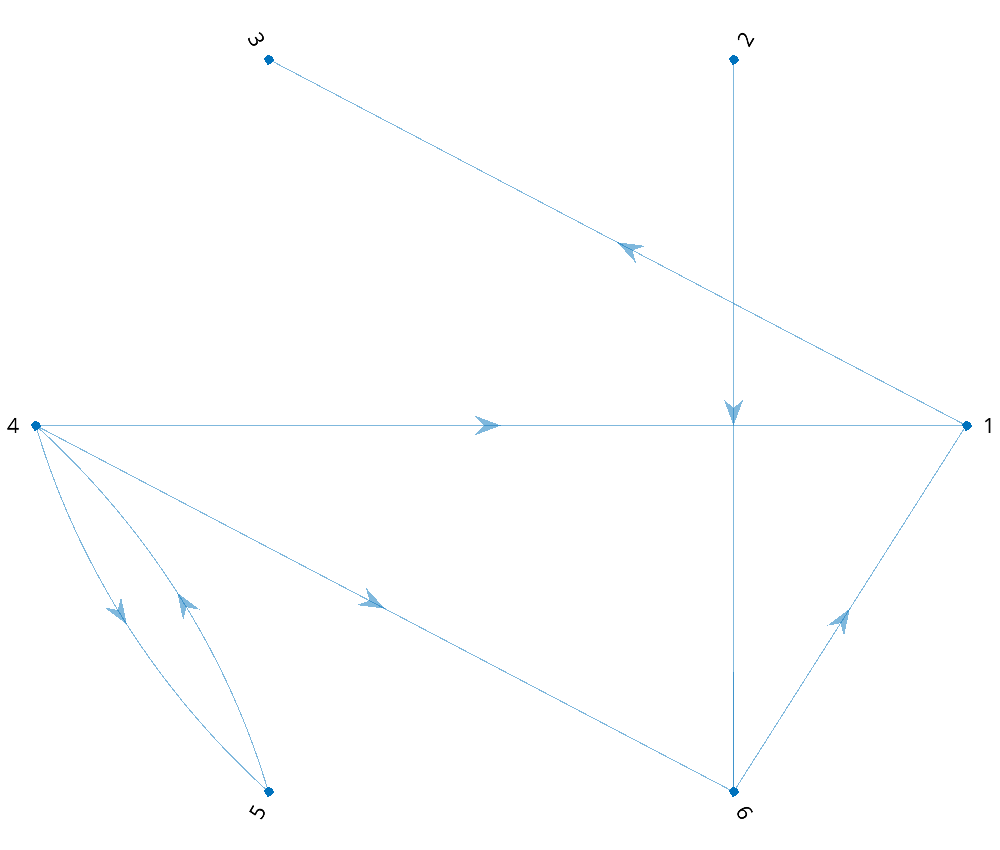
\includegraphics[scale=0.9]{../figures/A1_graph.png}
\end{center}

Vediamo quindi che le adiacenze fra nodi (pensando alla matrice, le dipendenze riga-colonna) sono:
\begin{table}[h!]
	\center \rowcolors{2}{white}{black!10}
	\begin{tabular} { c || c | c }
		\bfseries Nodo & \bfseries Raggiungibile & \bfseries Non raggiungibile \\
		\hline 
		1 & 1 3 & 2 4 5 6 \\
		2 & 1 2 3 6 & 4 5 \\
		3 & 3 & 1 2 4 5 6 \\
		4 & 1 3 4 5 6 & 2 \\
		5 & 1 3 4 5 6 & 2 \\
		6 & 1 3 6 & 2 4 5
	\end{tabular}
\end{table}

Notiamo che il nodo 6 ci fornisce la partizione migliore: $3 \times 3$ e $3 \times 3$.
Decidiamo quindi di prendere:
$$
\mathcal{P} = \{ 1, 3, 6 \}, \quad \mathcal{Q} = \{ 2, 4, 5 \}
$$
per cui la permutazione che manda $\mathcal{Q}$ in testa è:
$$
\Pi = \begin{pmatrix}
	0 & 1 & 0 & 0 & 0 & 0 \\
	0 & 0 & 0 & 1 & 0 & 0 \\
	0 & 0 & 0 & 0 & 1 & 0 \\
	1 & 0 & 0 & 0 & 0 & 0 \\
	0 & 0 & 1 & 0 & 0 & 0 \\
	0 & 0 & 0 & 0 & 0 & 1 \\
\end{pmatrix}
\begin{array}{c}
	2 \rightarrow 1 \\
	4 \rightarrow 2 \\
	5 \rightarrow 3 \\
	1 \rightarrow 4 \\
	3 \rightarrow 5 \\
	6 \rightarrow 6 \\
\end{array}
$$

Applicando $Pi A \Pi^T$ si ottiene quindi:
$$
\Pi A \Pi^T = \begin{pmatrix}
	A_{11} =
	\begin{pmatrix}
		2 &  0 &  0 \\
		0 &  2 & -1 \\
		0 & -1 &  2
	\end{pmatrix} &
	A_{12} = 
	\begin{pmatrix}
		0 &  0 &  3 \\
		3 &  0 & -2 \\
		0 &  0 &  0
	\end{pmatrix} \\
	0 &
	A_{21} = 
	\begin{pmatrix}
		1 &  1 &  0 \\
		0 & -1 &  0 \\
		1 &  0 &  1
	\end{pmatrix}
\end{pmatrix}
$$
che è una forma più agile per la risoluzione della matrice originale $A$.

Nella sottodirectory \lstinline|/code/matlab| si rende disponibile uno script \lstinline|block_decomp.m| per la decomposizione in matrici a blocchi come nell'esempio.
Un'esecuzione tipica dello script potrebbe avere l'aspetto:
\begin{lstlisting}[language=matlab, style=codestyle]	
p = block_decomp(A) % ottieni una permutazione
    Node      Reachable      Not reachable
    ____    _____________    _____________

     1      {[      1 3]}    {[  2 4 5 6]}
     2      {[  1 2 3 6]}    {[      4 5]}
     3      {[        3]}    {[1 2 4 5 6]}
     4      {[1 3 4 5 6]}    {[        2]}
     5      {[1 3 4 5 6]}    {[        2]}
     6      {[    1 3 6]}    {[    2 4 5]}
   
	 Choose an index: 6 % chiesto dallo script
>> A(p, p) % permuta A
\end{lstlisting}
da cui si ottiene la stessa matrice a blocchi riportata sopra.

\subsubsection{Riduzione iterata}
Ricordiamo di poter iterare ricorsivamente il processo di riduzione, cioè di poter trovare per ogni blocco $A_{ii}$ con $i \in \{ 1, 2 \}$ un $\Pi_i$ tale che:
$$
\Pi_i A_{ii} \Pi_i^T = \begin{pmatrix}
	A_{11}^{(i)} & A_{12}^{(i)} \\
	0 & A_{22}^{(i)} \\
\end{pmatrix}
$$
così che valga:
$$
\begin{pmatrix}
	\Pi_1 & 0 \\
	0 & \Pi_2
\end{pmatrix}
\begin{pmatrix}
	A_{11} & A_{12} \\
	0 & A_{22}
\end{pmatrix}
\begin{pmatrix}
	\Pi_1^T & 0 \\
	0 & \Pi_2^T
\end{pmatrix} =
\begin{pmatrix}
	\Pi_1 A_{11} \Pi_1^t & \Pi_1 A_{12} \Pi_2^T \\
	0 & \Pi_2 A_{22} \Pi_2^t \\
\end{pmatrix}
$$
$$
= \begin{pmatrix}
\begin{pmatrix}
	A_{11}^{(1)} & A_{12}^{(1)} \\
	0 & A_{22}^{(1)} \\
\end{pmatrix} & * \\
0 & 
\begin{pmatrix}
	A_{11}^{(2)} & A_{12}^{(2)} \\
	0 & A_{22}^{(2)} \\
\end{pmatrix}
\end{pmatrix}
$$
e via dicendo,
dove in $(*)$ comparrà qualcosa che al momento non ci interessa.

\subsubsection{Problemi agli autovalori per riduzione}
Notiamo che questo procedimento semplifica anche la risoluzione dei \textbf{problemi agli autovalori}: infatti iterando abbastanza, il problema si ridurrà a trovare i singoli autovalori di matrici sulla diagonale sempre più piccole, e quindi dal polinomio caratteristico di più facile risoluzione.

\subsection{Sistemi lineari}
Veniamo quindi alla trattazione dei sistemi lineari, che avevamo definito come forme $Ax = b$ con $A \in \mathbb{C}^{n \times n}, b \in \mathbb{C}^n$.

Studieremo 2 tipi di metodi risolutivi:
\begin{itemize}
	\item \textbf{Metodi diretti:} esatti ma dispendiosi, se eseguiti in aritmetica esatta (cioè senza arrotondamenti) poterebbero in un numero $n$ finito di passaggi alla soluzione esatta.
	Esempi di metodi diretti sono il \textbf{metodo di Cramer} (visto in 4.7.2) e l'\textbf{eliminazione di Gauss} (che vedremo fra poco);
	\item \textbf{Metodi iterativi:} meno accurati ma più efficienti computazionalmente, portano ad una successione $\{x_k\}_{k \in \mathbb{N}}$ di approssimazioni tali che $ \lim_{k \rightarrow +\infty} x_k = x$ soluzione esatta. Notiamo però che, in generale, è impossibile trovare il valore esatto di $x$ in un numero esatto di iterazioni. Per contropartita, risultano spesso molto più efficienti dei metodi diretti (esistono esempi di sistemi addirittura non risolvibili, nella pratica, con metodi diretti). 
\end{itemize}

\subsection{Metodi diretti per i sistemi lineari}
Iniziamo a trattare i metodi diretti per la risoluzione dei sistemi lineari.

\subsubsection{Sistemi triangolari}
Diamo la definizione parallela a quella di matrice triangolare:
\begin{definition}{Sistema triangolare}
	Si dice sistema triangolare un sistema della forma $Ux = c$ con $U$ matrice triangolare.
\end{definition}

Per un \textbf{sistema triangolare superiore}, si avrà la forma:
\[
\begin{cases}
    \begin{aligned}
			&& u_{11} x_1 + u_{12} x_2 + ... + u_{1,n-1} x_{n-1} + u_{1n} x_n = c_1 \\
			&&              u_{22} x_2 + ... + u_{2,n-1} x_{n-1} + u_{2n} x_n = c_2 \\
			&& \vdots \\
			&&                                 u_{n-1,n-1} x_{n-1} + u_{n-1,n} x_n = c_{n-1} \\
			&&                                                     u_{nn} x_n = c_n
		\end{aligned}
\end{cases}
\]

Il \textbf{metodo risolutivo} sarà allora la \textit{sostituzione all'indietro}, definita ricorsivamente come:
\[
	\begin{cases}
		x_n = \frac{c_n}{u_{nn}} \\\\ 
		x_i = \frac{ c_i - \sum_{j = i + 1}^n u_{ij} x_j }{u_{ii}}
	\end{cases}
\]
che equivale all'algoritmo, in MATLAB:
\lstinputlisting{../code/matlab/bck_subst.m}

Riguardo alla complessità, si potra dire che al passo $i$ si eseguono $n - i + n - i + 2 = 2(n - 1) + 2$ passaggi, cioè 2 per la divisione per $u_{jj}$ e la somma fra $c_i$ e il termine accumulato a destra, $n - i$ per i prodotti nella sommatoria e di nuovo $n - i$ per la sommatoria stessa.
Sarà allora che:
$$
\sum_{i = 1}^n \left( 2(n - i) + 2 \right) \sim O(n^2)
$$
cioè si ha complessità quadratica.

Osserviamo poi che per \textbf{sistemi triangolari inferiori} la situazione è uguale, cioè si risolve la prima equazione, si sostituisce il risultato nella seconda, e via dicendo:
\[
	\begin{cases}
		x_1 = \frac{c_1}{u_{11}} \\\\ 
		x_i = \frac{ c_i - \sum_{j = 1}^{i - 1} u_{ij} x_j }{u_{ii}}
	\end{cases}
\]
che equivale all'algoritmo, in MATLAB:
\lstinputlisting{../code/matlab/fwd_subst.m}

Il metodo ottenuto, speculare al quello di sostituzione all'indietro, viene detto \textit{sostituzione in avanti}, di costo identico ($O(n^2)$).

\subsubsection{Metodo di eliminazione di Gauss}
L'idea del metodo di eliminazione di Gauss è quella di partire da un sistema $Ax = b$, trasformarlo in un sistema equivalente $Ux = c$ (quindi triangolare superiore), ed applicare la sostituzione all'indietro.

Per arrivare alla forma $Ux = c$ si sostituiscono le equazioni del sistema con loro combinazioni lineari scelte in modo da annullare gli elementi inferiori alla diagonale.

L'idea è quella di eliminare, per ogni elemento $i$-esimo sulla diagonale a partire da quello in alto a destra, gli $n - i$ elementi che stanno al di sotto, cioè:

\begin{algorithm}
\caption{Eliminazione di Gauss}
\begin{algorithmic}
	\STATE \textbf{Input:} un sistema lineare qualsiasi $Ax = b$ % input
	\STATE \textbf{Output:} un sistema lineare triangolare superiore $Ux = c$ % output
	% body
	\FOR{$i = 1$ to $n$}
		\FOR{$j = i$ to $n$}
			\STATE Calcola il \textbf{moltiplicatore} $l_{ji} = \frac{a_{ji}^{(i - 1)}}{a_{ii}^{(i - 1)}}$
			\STATE Aggiungi alla riga $j$ la riga $i$ moltiplicata per $l_{ij}$
		\ENDFOR
	\ENDFOR
\end{algorithmic}
\end{algorithm}

\subsubsection{Implementazione MATLAB del metodo di eliminazione Gauss}
Una semplice implementazione in MATLAB del suddetto algoritmo può essere la seguente:
\begin{lstlisting}[language=matlab, style=codestyle]	
function [A, b] = gauss_decomp(A, b)
    n = height(A);

    for i = 1:n % i itera sulle diagonali
        den = A(i, i);

        for j = (i + 1):n % j itera sulle righe
            mul = A(j, i) / den; % moltiplicatore
            
            A(j, :) = A(j, :) - A(i, :) * mul;
            b(j) = b(j) - b(i) * mul;
        end
    end
end
\end{lstlisting}
da cui si potrà ottenere una riduzione di Gauss semplicemente come:
\begin{lstlisting}[language=matlab, style=codestyle]	
	>> [U, c] = gauss_decomp(A, b)
\end{lstlisting}

\par\smallskip

Dal punto di vista della complessità, la riduzione in forma triangolare costa $O(\frac{2}{3}n^3)$, e chiaramente domina sul termine $O(n^2)$ della risoluzione di $Ux = c$ con la sostituzione all'indietro.

Facciamo una nota sulla fattibiltà della riduzione di Gauss, definendo:
\begin{definition}{Moltiplicatori di Gauss}
	I termini $l_{ji} = \frac{a_{ji}^{(i - 1)}}{a_{ii}^{(i - 1)}}$ vengono detti moltiplicatori.
\end{definition}
Chiaramente, per poter eseguire l'eliminazione di Gauss serve che $a_{jj^{j - 1}} \neq 0$ $\forall j = 1, ..., n - 1$.
Inoltre, i casi $a_{jj}^{j - 1} \approx 0$ possono causare problemi di instabilità numerica.
Vedremo in seguito metodi per ovviare a questo problema.

\subsubsection{Fattorizzazione LU}
Il primo passo dell'algoritmo di Gauss si può vedere come equivalente a moltiplicare l'equazione $Ax = b$ a sinistra per una particolare matrice $H_1$ triangolare inferiore:
$$
H_1 = \begin{pmatrix}
	1 & ... & ... & 0 \\
	-l_{21} & 1 & ... & 0 \\
	... \\ 
	-l_{n1} & ... & ... & 1
\end{pmatrix}
$$
con la diagonale a $1$ e i moltiplicatori sulla prima colonna, così che $H_1 A$ risulti esattamente quello che volevamo per Gauss, cioè la combinazione lineare di ogni riga $j$ con l'prima riga moltiplicata per il moltiplicatore $l_{j1}$ (con $j > 2$).

Possiamo generalizzare questo processo a una serie di matrici $H_i$, per ogni elemento sulla diagonale, con la diagonale a $1$ e i moltiplicatori corrispondenti a $i$ sulla $i$-esima colonna:
$$
H_i = \begin{pmatrix}
	1 & ... & ... & 0 \\
	0 & 1 & ... & 0 \\
	... & -l_{ji} & ... & ... \\
	0 & -l_{ni} & ... & 1
\end{pmatrix}
$$
Così, ancora una volta, $A H_i$ risulterà quello che volevamo per Gauss, cioè la combinazione lineare di ogni riga $j$ con l'$i$-esima riga moltiplicata per il moltiplicatore $l_{ji}$.

Varrà allora he il metodo di Gauss sarà equivalente a considerare:
$$
H_{n - 1} H_{n - 2} \, ... \, H_1 A x = H_{n - 1} H_{n - 2} \, ... \, H_1 b
$$
e potremo quindi dire:
$$
H_{n - 1} H_{n - 2} \, ... \, H_1 A = U, \quad L = H_1^{-1} \, ... \, H_{n - 1}^1 
$$
da cui:
$$
A = LU
$$

Semplifichiamo i calcoli notando alcune proprietà delle matrici $H_j$:
\begin{enumerate}
	\item Hanno l'inversa facile, in quanto basta invertire i segni:
	$$
	H_i^{-1} = \begin{pmatrix}
		1 & ... & ... & 0 \\
		0 & 1 & ... & 0 \\
		... & l_{ji} & ... & ... \\
		0 & l_{ni} & ... & 1
	\end{pmatrix}
	$$

	\item Sono facili da moltiplicare, in quanto si può dire:
	$$
		H_{i_1} \cdot H_{i_2} = \begin{pmatrix}
		1 & ... & ... & 0 \\
		-l_{2i_1} & 1 & ... & 0 \\
		... & -l_{ji_2} & ... & ... \\
		-l_{ni_i} & -l_{ni_2} & ... & 1
	\end{pmatrix}
	$$
	e:	
	$$
	H_{i_1}^{-1} \cdot H_{i_2}^{-1} = \begin{pmatrix}
		1 & ... & ... & 0 \\
		l_{2i_1} & 1 & ... & 0 \\
		... & l_{ji_2} & ... & ... \\
		l_{ni_i} & l_{ni_2} & ... & 1
	\end{pmatrix}
	$$

	cioè semplicemente si somma sotto la diagonale.
\end{enumerate}

Questo significa che una volta svolta la prima parte dell'eliminazione di Gauss si è gia calcolata la fattorizzazione LU come la matrice dei moltiplicatori:
$$
H_{i_1}^{-1} \cdot H_{i_2}^{-1} = \begin{pmatrix}
	1 & ... & ... & 0 \\
	l_{21} & 1 & ... & 0 \\
	... & l_{3,2} & ...\\
	l_{n1} & l_{n2} & ... & 1
\end{pmatrix}
$$

\subsubsection{Implementazione MATLAB della riduzione LU}
Modifichiamo il codice MATLAB della scorsa sezione per calcolare, oltre all'eliminazione di Gauss (cioè la matrice $U$), la matrice dei moltiplicatori $L$:
\begin{lstlisting}[language=matlab, style=codestyle]	
function [A, b, L] = gauss_decomp(A, b)
    n = height(A);

    L = eye(n); % prepara L

    for i = 1:n % i itera sulle diagonali
        den = A(i, i);

        for j = (i + 1):n % j itera sulle righe
            mul = A(j, i) / den; % moltiplicatore
            L(j, i) = mul;
            
            A(j, :) = A(j, :) - A(i, :) * mul;
            b(j) = b(j) - b(i) * mul;
        end
    end
end
\end{lstlisting}

A questo punto per calcolare la fattorizzazione LU di una matrice basterà eseguire:
\begin{lstlisting}[language=matlab, style=codestyle]	
>> [U, ~, L] = gauss_decomp(A, b)
>> L * U % idealmente dara' A
\end{lstlisting}

\par\medskip

Si osserva quindi che se già si conoscono $L$ ed $U$ (magari di una matrice che dovremo usare spesso) risolvere $Ax = b$ costa $O(n^2)$, in quanto basta dire:
$$
Ax = b \, \Rightarrow \, LUx = b \implies x = U^{-1} L^{-1} b
$$
dove basta risolvere a cascata:
\[
	\begin{cases}
		Ly = b \\\
		Ux = y
	\end{cases}
\]
Questi sono due sistemi triangolari, uno \textbf{inferiore} (risolvibile per \textit{sostituzione in avanti}), l'altro \textbf{superiore} (risolvibile per \textit{sostituzione all'indietro}), da cui l'andamento complessivo $O(n^2)$.

In MATLAB, la soluzione si può quindi avere usando le funzioni definite finora:
\begin{lstlisting}[language=matlab, style=codestyle]	
>> [U, ~, L] = gauss_decomp(A, b)
>> y = fwd_subst(L, b)
>> x = bck_subst(U, y) % x e' la soluzione del sistema
\end{lstlisting}

Notiamo che questo vale se $L$ ed $U$ sono note (o come nell'esempio vengono calcolate), quindi tolto il prezzo dato dal doverle calcolare (come avevamo notato, conviene per matrici che magari dobbiamo usare spesso).

\subsubsection{Metodo di Gauss per variabili matriciali}
Se si vuole risolvere $AX = B$ con $X$ e $B$ matrici di vettori colonna di $s$ colonne:
$$
X = \begin{pmatrix}
	x_1 & ... & x_s
\end{pmatrix}, \quad
B = \begin{pmatrix}
	b_1 & ... & b_s
\end{pmatrix}
$$
cioè se si vogliono risolvere $s$ sistemi lineari con la stessa matrice $A$:
$$
Ax_1 = b_1, \quad ..., \quad Ax_s = b_s
$$
si può modificare l'algoritmo di Gauss, effettuando le mosse di Gauss sulla matrice aumentata $\begin{pmatrix}
	A \, | \, B
\end{pmatrix}$.
Alla fine troveremo una matrice $\begin{pmatrix}
	U \, | \, B^{(n - 1)}
\end{pmatrix}$, dove gli apici $(n - 1)$ rappresentano che è la $B$ che si ottiene all'$n-1$-esimo passaggio, che risolverà i sistemi triangolari superiori:
$$
Ux_1 = b_1^{(n - 1)}, \quad ..., \quad Ux_s = b_s^{(n - 1)}
$$

\par\smallskip

Vediamo un esempio numerico.
Partiamo dalle matrici $A$ e $B$:
$$
A = \begin{pmatrix}
	-2 & 1 & 1 \\ 
	-1 & 3 & 1 \\ 
	1 & 1 & 2
\end{pmatrix}, \quad B = \begin{pmatrix}
	-2 & 0 \\ 
	-3 & 0 \\ 
	2 & 1
\end{pmatrix}
$$
Avremo che le due colonne di $B$ rappresentano due vettori "termini noti" diversi, e che quindi la soluzione $X$ di $AX = B$ rappresenterà in verità due vettori soluzione:
$$
X = \begin{pmatrix}
	x_1^{(1)} & x_1^{(2)} \\
	x_2^{(1)} & x_2^{(2)} \\
	x_3^{(1)} & x_3^{(2)} \\
\end{pmatrix}
$$

Costruiamo quindi la matrice $AB$ ed applichiamo il metodo di riduzione di Gauss:
$$
AB = 
\left(\begin{array}{@{}c c c | c c@{}}
	-2 & 1 & 1 & -2 & 0 \\
	-1 & 3 & 1 & -3 & 0 \\
	1 & 1 & 2 & 2 & 1
\end{array}\right) \xrightarrow{\text{Gauss}}
\left(\begin{array}{@{}c c c | c c@{}}
	-2 & 1 & 1 & -2 & 0 \\
	0 & \frac{5}{2} & \frac{1}{2} & -2 & 0 \\ 
	0 & 0 & \frac{11}{5} & \frac{11}{5} & 1
\end{array}\right) = UB^{(n - 1)}
$$

Avremo quindi due sistemi dati dalla forma $UX = B^{(n - 1)}$:

\begin{minipage}{0.45\textwidth}

	\[
		x^{(1)} :
		\begin{cases}
			-2 x_1^{(1)} + x_2^{(1)} + x_3^{(1)} = -2 \\ 
			\frac{5}{2} x_2^{(1)} + \frac{1}{2} x_3^{(1)} = -2 \\ 
			\frac{11}{5} x_3^{(1)} = \frac{11}{5}
		\end{cases}
	\]

\end{minipage}%
\hfill % This adds horizontal space between the two minipages
\begin{minipage}{0.45\textwidth}

	\[
		x^{(2)} :
		\begin{cases}
			-2 x_1^{(2)} + x_2^{(2)} + x_3^{(2)} = 0 \\ 
			\frac{5}{2} x_2^{(2)} + \frac{1}{2} x_3^{(2)} = 0 \\ 
			\frac{11}{5} x_3^{(2)} = 1
		\end{cases}
	\]

\end{minipage}

da cui le soluzioni:
$$
x^{(1)} = \begin{pmatrix}
	1 \\ -1 \\ 1
\end{pmatrix} \quad 
x^{(2)} = \begin{pmatrix}
	\frac{2}{11} \\ -\frac{1}{11} \\ \frac{5}{11}
\end{pmatrix}
$$
e quindi la matrice incognita $X$:
$$
X = \begin{pmatrix}
	1 & \frac{2}{11} \\
	-1 & -\frac{1}{11} \\
	1 & \frac{5}{11} \\
\end{pmatrix}
$$


\subsubsection{Implementazione MATLAB del metodo di Gauss}
Implementiamo un risolutore per sistemi lineari, per comprendere a pieno questo risultato.
Vogliamo calcolare $X$ come la soluzione del sistema $AX = B$, e capiamo quindi che quello che cerchiamo sono i vettori colonna $x_1, ..., x_n$ tali per cui:
$$
A x_1 = B_1, \quad ..., \quad A x_n = b_n
$$
con $b_i$ l'$i$-esimo vettore colonna di $B$.
Sfruttiamo allora l'eliminazione di Gauss per ricavare due matrici, $U$ e $B^{(n - 1)}$, tali che $Ux = B^{(n - 1)}$, con il vantaggio che $U$ è triangolare superiore e quindi risolvibile per sostituzione all'indietro.
Possiamo fare questo in MATLAB come:
\begin{lstlisting}[language=matlab, style=codestyle]	
AI = [A, B]
UB1 = gauss_decomp(AB) % modificando gauss_decomp per un solo argomento 
U = UB1(1:n, 1:n)
B1 = UB1(1:n, (n + 1):(n + s)
\end{lstlisting}

A questo punto potremo trovare le colonne $x_i$ come:
\begin{lstlisting}[language=matlab, style=codestyle]	
>> x1 = bck_subst(U, B1(1:n, 1))
>> x2 = bck_subst(U, B1(1:n, 2))
...
\end{lstlisting}
e infine concatenare le colonne come:
\begin{lstlisting}[language=matlab, style=codestyle]	
>> X = [x1, ..., xn]
\end{lstlisting}
che realizzato in un unico script risulta:
\lstinputlisting{../code/matlab/gauss_solve.m}

\subsubsection{Metodo di Gauss per il calcolo dell'inversa}
Un caso particolare è il \textbf{calcolo dell'inversa} con l'algoritmo di \textbf{Gauss-Jordan}.
Infatti, scegliendo:
$$
AX = I
$$
con $n = s$, le colonne in $X$ diventeranno l'inversa di $A$ (basti vedere che $A A^{-1} = I$ per definizione).

\par\smallskip

Facciamo un esempio numerico.
Prendiamo la stessa matrice di prima:
$$
A = \begin{pmatrix}
	-2 & 1 & 1 \\ 
	-1 & 3 & 1 \\ 
	1 & 1 & 2
\end{pmatrix}
$$
e calcoliamone l'inversa come soluzione a $AX = I$.
Impostiamo quindi la matrice $AI$ e riduciamola:
$$
AI = 
\left(\begin{array}{@{}c c c | c c c@{}}
		-2 & 1 & 1 & 1 & 0 & 0 \\
		-1 & 3 & 1 & 0 & 1 & 0 \\
		1 & 1 & 2 & 0 & 0 & 1
\end{array}\right) \xrightarrow{\text{Gauss}}
\left(\begin{array}{@{}c c c | c c c @{}}
		-2 & 1 & 1 & 1 & 0 & 0 \\
		0 & \frac{5}{2} & \frac{1}{2} & -\frac{1}{2} & 1 & 0 \\ 
	0 & 0 & \frac{11}{5} & \frac{4}{5} & -\frac{3}{5} & 1
\end{array}\right) = UB^{(n - 1)}
$$
da cui i 3 sistemi lineari:

\begin{minipage}{0.35\textwidth}

	\[
	x^{(1)} :
		\begin{cases}
			-2 x_1^{(1)} + x_2^{(1)} + x_3^{(1)} = 1 \\ 
			\frac{5}{2} x_2^{(1)} + \frac{1}{2} x_3^{(1)} = -\frac{1}{2} \\ 
			\frac{11}{5} x_3^{(1)} = \frac{4}{5}
		\end{cases}
	\]

\end{minipage}%
\hfill
\begin{minipage}{0.35\textwidth}

	\[
	x^{(2)} :
		\begin{cases}
			-2 x_1^{(2)} + x_2^{(2)} + x_3^{(2)} = 0 \\ 
			\frac{5}{2} x_2^{(2)} + \frac{1}{2} x_3^{(2)} = 1 \\ 
			\frac{11}{5} x_3^{(2)} = -\frac{3}{5}
		\end{cases}
	\]

\end{minipage}
\[
x^{(3)} :
	\begin{cases}
		-2 x_1^{(3)} + x_2^{(3)} + x_3^{(3)} = 0 \\ 
		\frac{5}{2} x_2^{(3)} + \frac{1}{2} x_3^{(3)} = 0 \\ 
		\frac{11}{5} x_3^{(3)} = 1
	\end{cases}
\]
che hanno come soluzione:
$$
X = \begin{pmatrix}
	x^{(1)} & x^{(2)} & x^{(3)}
\end{pmatrix} = A^{-1} = \begin{pmatrix}
	-\frac{5}{11} & \frac{1}{11} & \frac{2}{11} \\ 
	-\frac{3}{11} & \frac{5}{11} & -\frac{1}{11} \\ 
	\frac{4}{11} & -\frac{3}{11} & \frac{5}{11}
\end{pmatrix}
$$

\subsubsection{Implementazione MATLAB del metodo di Gauss per il calcolo dell'inversa}
Facciamo un ultimo esempio MATLAB di questo procedimento.
Vogliamo calcolare $A^{-1}$ come la soluzione del sistema $AX = I$, e capiamo quindi che quello che cerchiamo sono i vettori colonna $i_1, ..., i_n$ tali per cui:
$$
A i_1 = I_1, \quad ..., \quad A i_n = I_n
$$
	con $I_i$ il vettore di zeri con un 1 all'$i$-esima riga. 
	Anche allora vogliamo sfruttare l'eliminazione di Gauss per ricavare due matrici, $U$ e $B^{(n - 1)}$, tali che $Ux = B^{(n - 1)}$, con il vantaggio che $U$ è triangolare superiore e quindi risolvibile per sostituzione all'indietro.

	Questo è esattamente quello che ci permette di fare la funzione \lstinline|gauss_solve()| definita prima, fissando il secondo argomento all'identità $I$ (in matlab \lstinline|eye(n)|):
	\lstinputlisting{../code/matlab/gauss_inv.m}

\end{document}


\documentclass[a4paper,11pt]{article}
\usepackage[a4paper, margin=8em]{geometry}

% usa i pacchetti per la scrittura in italiano
\usepackage[french,italian]{babel}
\usepackage[T1]{fontenc}
\usepackage[utf8]{inputenc}
\frenchspacing 

% usa i pacchetti per la formattazione matematica
\usepackage{amsmath, amssymb, amsthm, amsfonts}

% usa altri pacchetti
\usepackage{gensymb}
\usepackage{hyperref}
\usepackage{standalone}

% imposta il titolo
\title{Appunti Calcolo Numerico}
\author{Luca Seggiani}
\date{2025}

% disegni
\usepackage{pgfplots}
\pgfplotsset{width=10cm,compat=1.9}

% imposta lo stile
% usa helvetica
\usepackage[scaled]{helvet}
% usa palatino
\usepackage{palatino}
% usa un font monospazio guardabile
\usepackage{lmodern}

% tikz in sans
\tikzset{every picture/.style={/utils/exec={\sffamily}}}

\renewcommand{\rmdefault}{ppl}
\renewcommand{\sfdefault}{phv}
\renewcommand{\ttdefault}{lmtt}

% circuiti
\usepackage{circuitikz}
\usetikzlibrary{babel}

% disponi il titolo
\makeatletter
\renewcommand{\maketitle} {
	\begin{center} 
		\begin{minipage}[t]{.8\textwidth}
			\textsf{\huge\bfseries \@title} 
		\end{minipage}%
		\begin{minipage}[t]{.2\textwidth}
			\raggedleft \vspace{-1.65em}
			\textsf{\small \@author} \vfill
			\textsf{\small \@date}
		\end{minipage}
		\par
	\end{center}

	\thispagestyle{empty}
	\pagestyle{fancy}
}
\makeatother

% disponi teoremi
\usepackage{tcolorbox}
\newtcolorbox[auto counter, number within=section]{theorem}[2][]{%
	colback=blue!10, 
	colframe=blue!40!black, 
	sharp corners=northwest,
	fonttitle=\sffamily\bfseries, 
	title=Teorema~\thetcbcounter: #2, 
	#1
}

% disponi definizioni
\newtcolorbox[auto counter, number within=section]{definition}[2][]{%
	colback=red!10,
	colframe=red!40!black,
	sharp corners=northwest,
	fonttitle=\sffamily\bfseries,
	title=Definizione~\thetcbcounter: #2,
	#1
}

% disponi problemi
\newtcolorbox[auto counter, number within=section]{problem}[2][]{%
	colback=green!10,
	colframe=green!40!black,
	sharp corners=northwest,
	fonttitle=\sffamily\bfseries,
	title=Problema~\thetcbcounter: #2,
	#1
}

% disponi codice
\usepackage{listings}
\usepackage[table]{xcolor}

\definecolor{codegreen}{rgb}{0,0.6,0}
\definecolor{codegray}{rgb}{0.5,0.5,0.5}
\definecolor{codepurple}{rgb}{0.58,0,0.82}
\definecolor{backcolour}{rgb}{0.95,0.95,0.92}

\lstdefinestyle{codestyle}{
		backgroundcolor=\color{black!5}, 
		commentstyle=\color{codegreen},
		keywordstyle=\bfseries\color{magenta},
		numberstyle=\sffamily\tiny\color{black!60},
		stringstyle=\color{green!50!black},
		basicstyle=\ttfamily\footnotesize,
		breakatwhitespace=false,         
		breaklines=true,                 
		captionpos=b,                    
		keepspaces=true,                 
		numbers=left,                    
		numbersep=5pt,                  
		showspaces=false,                
		showstringspaces=false,
		showtabs=false,                  
		tabsize=2
}

\lstdefinestyle{shellstyle}{
		backgroundcolor=\color{black!5}, 
		basicstyle=\ttfamily\footnotesize\color{black}, 
		commentstyle=\color{black}, 
		keywordstyle=\color{black},
		numberstyle=\color{black!5},
		stringstyle=\color{black}, 
		showspaces=false,
		showstringspaces=false, 
		showtabs=false, 
		tabsize=2, 
		numbers=none, 
		breaklines=true
}

\lstdefinelanguage{javascript}{
	keywords={typeof, new, true, false, catch, function, return, null, catch, switch, var, if, in, while, do, else, case, break},
	keywordstyle=\color{blue}\bfseries,
	ndkeywords={class, export, boolean, throw, implements, import, this},
	ndkeywordstyle=\color{darkgray}\bfseries,
	identifierstyle=\color{black},
	sensitive=false,
	comment=[l]{//},
	morecomment=[s]{/*}{*/},
	commentstyle=\color{purple}\ttfamily,
	stringstyle=\color{red}\ttfamily,
	morestring=[b]',
	morestring=[b]"
}

% disponi sezioni
\usepackage{titlesec}

\titleformat{\section}
	{\sffamily\Large\bfseries} 
	{\thesection}{1em}{} 
\titleformat{\subsection}
	{\sffamily\large\bfseries}   
	{\thesubsection}{1em}{} 
\titleformat{\subsubsection}
	{\sffamily\normalsize\bfseries} 
	{\thesubsubsection}{1em}{}

% disponi alberi
\usepackage{forest}

\forestset{
	rectstyle/.style={
		for tree={rectangle,draw,font=\large\sffamily}
	},
	roundstyle/.style={
		for tree={circle,draw,font=\large}
	}
}

% disponi algoritmi
\usepackage{algorithm}
\usepackage{algorithmic}
\makeatletter
\renewcommand{\ALG@name}{Algoritmo}
\makeatother

% disponi numeri di pagina
\usepackage{fancyhdr}
\fancyhf{} 
\fancyfoot[L]{\sffamily{\thepage}}

\makeatletter
\fancyhead[L]{\raisebox{1ex}[0pt][0pt]{\sffamily{\@title \ \@date}}} 
\fancyhead[R]{\raisebox{1ex}[0pt][0pt]{\sffamily{\@author}}}
\makeatother

\begin{document}

% sezione (data)
\section{Lezione del 24-03-25}

% stili pagina
\thispagestyle{empty}
\pagestyle{fancy}

% testo
\subsection{Pivoting}
L'algoritmo di eliminazione di Gauss che abbiamo definito alla scorsa lezione ha un punto di fallimento nel caso uno degli elementi $a_{ii}^{(i - 1)}$ sia $= 0$, o comunque $\approx 0$, in quanto vorremmo a quel punto calcolare un moltiplicatore $l_{ji} = \frac{a_{ji}}{a_{ii}} \rightarrow$ non ben definito.

In tal caso si può modificare l'algoritmo sfruttando una matrice di permutazione che porti un elemento diverso da zero nella stessa posizione di $a_{ii}$.
Vorremo quindi cercare un indice $h$ tal per cui $a_{hi}^{(i - 1)}$ sia di modulo massimo nella sua colonna al di sotto di $i$, cioè:
$$
a_{hi}^{(i - 1)} \geq \max_{j = i, ..., n} | a_{ji}^{(i - 1)} |
$$
e scambiare la riga $i$ con la riga $h$.
Infatti, se $\det(A) \neq 0$, allora necessariamente esiste un $a_{ji}^{(i - 1)} \neq 0$ (altrimenti si ha uno 0 obbligato sulla diagonale, che con la matrice triangolare a blocchi dà $\det(A^{(i - 1)}) = 0$). \qed

Un altra conseguenza di questo approccio è che tutti i moltiplicatori $l_{ji}$ diventeranno $\leq 1$.
L'algoritmo di Gauss con questa modifica si chiama \textbf{eliminazione di Gauss con pivoting parziale} (\textit{parziale} perché ne esistono versioni più sofisticate, che non vedremo).

Osserviamo che ogni scambio di righe equivale a moltiplicare a sinistra per una matrice di permutazione $\Pi_i$.
Quindi il metodo di Gauss con pivoting può essere rappresentato come:
\begin{algorithm}
\caption{Eliminazione di Gauss con pivoting parziale}
\begin{algorithmic}
	\STATE \textbf{Input:} un sistema lineare qualsiasi $Ax = b$ % input
	\STATE \textbf{Output:} un sistema lineare triangolare superiore $Ux = c$ % output
	% body
	\FOR{$i = 1$ to $n$}
		\STATE Trova la matrice $\Pi_i$ che porta l'elemento di modulo massimo in testa
		\STATE $A \leftarrow \Pi_i A$
		\FOR{$j = i$ to $n$}
			\STATE Calcola il \textbf{moltiplicatore} $l_{ji} = \frac{a_{ji}^{(i - 1)}}{a_{ii}^{(i - 1)}}$
			\STATE Aggiungi alla riga $j$ la riga $i$ moltiplicata per $l_{ij}$
		\ENDFOR
	\ENDFOR
\end{algorithmic}
\end{algorithm}

\par\smallskip

Vediamo un esempio pratico dell'algoritmo prima di procedere all'implementazione MATLAB.
Prendiamo la matrice $A$ e il vettore $b$:
$$
A = \begin{pmatrix}
	1 & 2 & 3 \\ 
	4 & 5 & 6 \\ 
	7 & 8 & 0
\end{pmatrix}, \quad
b = \begin{pmatrix}
	1 \\ 2 \\ 3
\end{pmatrix}
$$
Nel ridurre la matrice aumentata $Ab$:
$$
\left(\begin{array}{@{}c c c | c@{}}
	1 & 2 & 3 & 1 \\ 
	4 & 5 & 6 & 2 \\ 
	7 & 8 & 0 & 3
\end{array}\right)
$$
ci accorgiamo che alla prima colonna l'entrata di modulo massimo è 7, di indice 3. Si permutano quindi la prima e la terza riga:
$$
\xrightarrow{\Pi_1}
\left(\begin{array}{@{}c c c | c@{}}
	7 & 8 & 0 & 3 \\
	4 & 5 & 6 & 2 \\ 
	1 & 2 & 3 & 1
\end{array}\right)
\xrightarrow{H_1 \Pi_1}
\left(\begin{array}{@{}c c c | c@{}}
		7 & 8 & 0 & 3 \\ 
		0 & \frac{3}{7} & 6 & \frac{2}{7} \\ 
		0 & \frac{6}{7} & 3 & \frac{4}{7}
\end{array}\right)
$$
nuovamente, l'entrata di modulo massimo è all'indice 3. Si permutano quindi la seconda e la terza riga:
$$
\xrightarrow{\Pi_2 H_1 \Pi_1}
\left(\begin{array}{@{}c c c | c@{}}
		7 & 8 & 0 & 3 \\ 
		0 & \frac{6}{7} & 3 & \frac{4}{7} \\
		0 & \frac{3}{7} & 6 & \frac{2}{7} 
\end{array}\right)
\xrightarrow{H_2 \Pi_2 H_1 \Pi_1}
\left(\begin{array}{@{}c c c | c@{}}
		7 & 8 & 0 & 3 \\ 
		0 & \frac{6}{7} & 3 & \frac{4}{7} \\
		0 & 0 & \frac{9}{2} & 0
\end{array}\right)
$$

\subsubsection{Implementazione MATLAB del metodo di eliminazione di Gauss con pivoting}
Modifichiamo quindi la funzione \lstinline|gauss_decomp()| per introdurre il meccanismo di pivoting appena visto:
\begin{lstlisting}[language=matlab, style=codestyle]	
function [A, b] = gauss_decomp(A, b)
    n = height(A);

    if nargin < 2
        b = zeros(n, 1);
    end

    for i = 1:n % i itera sulle diagonali
        % qui fai il pivot
        max_abs = max(abs(A(i:n, i)));
        h = find(abs(A(i:n, i)) == max_abs, 1);
        h = h + i - 1; % max abs si conta da i in poi

        A([i, h], :) = A([h, i], :); % permuta A
        b([i, h]) = b([h, i]); % permuta b
        
        den = A(i, i);

        for j = (i + 1):n % j itera sulle righe
            mul = A(j, i) / den; % moltiplicatore
            L(j, i) = mul;
            
            A(j, :) = A(j, :) - A(i, :) * mul;
            b(j) = b(j) - b(i) * mul;
        end
    end
end
\end{lstlisting}

\subsubsection{Fattorizzazione LU con pivoting}
Vediamo come ricavare una fattorizzazione LU dal metodo di Gauss modificato con il pivoting.
Si ha quindi che la matrice $U$ si evolve come:
$$
A \rightarrow \Pi_1 A \rightarrow H_1 \Pi_1 A \rightarrow ... \rightarrow H_{n - 1} \Pi_{n - 1} ... H_1 \Pi_1 A = U 
$$
mentre per la $L$ dovremo notare che:
$$
LU = \Pi A
$$
dove la matrice $\Pi$ rappresenta tutte le permutazioni fatte sulle righe di $A$.

Si ha quindi che:
\begin{itemize}
	\item $U$ è la matrice triangolare superiore trovata alla fine del metodo di Gauss con pivoting;
	\item $L$ è la matrice dei moltiplicatori, a cui però si devono applicare gli scambi delle righe, come segue: se al passo $i$ applico la matrice $\Pi_i$, devo applicare lo stesso cambio nelle prime $i - 1$ colonne di $L$, sotto la diagonale.
\end{itemize}

\par\smallskip 

Vediamo un esempio numerico spieghi il processo di formazione della matrice $L$ e della matrice di permutazione $\Pi$.
Presa la stessa matrice dell'esempio precedente:
$$
A = \begin{pmatrix}
	1 & 2 & 3 \\ 
	4 & 5 & 6 \\ 
	7 & 8 & 0
\end{pmatrix}
$$
abbiamo che le permutazioni sono, in sequenza:
$$
\Pi_1 : 
\begin{pmatrix}
	1 \\ 2 \\ 3
\end{pmatrix}
\rightarrow
\begin{pmatrix}
	3 \\ 2 \\ 1
\end{pmatrix}, \quad 
\Pi_2 :
\begin{pmatrix}
	3 \\ 2 \\ 1
\end{pmatrix}
\rightarrow
\begin{pmatrix}
	3 \\ 1 \\ 2
\end{pmatrix}
$$
o, in forma matriciale:
$$
\Pi_1 = \begin{pmatrix}
	0 & 0 & 1 \\ 
	0 & 1 & 0 \\ 
	1 & 0 & 0
\end{pmatrix}, \quad
\Pi_2 = \begin{pmatrix}
	1 & 0 & 0 \\ 
	0 & 0 & 1 \\ 
	0 & 1 & 0
\end{pmatrix}
$$

Calcoliamo quindi $L$.
$\Pi_1$ è irrilevante al calcolo di $L$, quindi la ignoriamo.
Vediamo che i primi due moltiplicatori sono $l_{21} = \frac{4}{7}$ e $l_{31} = \frac{1}{7}$, da cui si imposta $L^{(1)}$:
$$
L^{(1)} = \begin{pmatrix}
	1 & 0 & 0 \\ 
	\frac{4}{7} & 1 & 0 \\ 
	\frac{1}{7} & 0 & 1
\end{pmatrix}
$$

Notiamo quindi che dalla $\Pi_2$ dobbiamo scambiare gli elementi sotto la diagonale della prima colonna, quindi:
$$
L^{(1)} = \begin{pmatrix}
	1 & 0 & 0 \\ 
	\frac{1}{7} & 1 & 0 \\ 
	\frac{4}{7} & 0 & 1
\end{pmatrix}
$$

Infine, l'ultimo moltiplicatore $l_{32} = \frac{1}{2}$ non ha ambiguità:
$$
L^{(2)} = L = \begin{pmatrix}
	1 & 0 & 0 \\ 
	\frac{1}{7} & 1 & 0 \\ 
	\frac{4}{7} & \frac{1}{2} & 1
\end{pmatrix}
$$

Il calcolo di $\Pi$ deriva invece direttamente studiando la permutazione complessiva data dalle $\Pi_1, ..., \Pi_{n - 1}$, in questo caso:
$$
\Pi : \begin{pmatrix}
	1 \\ 2 \\ 3
\end{pmatrix}
\xrightarrow{\Pi_1}
\begin{pmatrix}
	3 \\ 2 \\ 1
\end{pmatrix}
\xrightarrow{\Pi_2}
\begin{pmatrix}
	3 \\ 1 \\ 2
\end{pmatrix}
$$
da cui:
$$
\Pi = \begin{pmatrix}
	0 & 0 & 1 \\ 
	1 & 0 & 0 \\ 
	0 & 1 & 0
\end{pmatrix}
$$

Con brevi calcoli si verifica che:
$$
LU = \Pi A
$$

\par\medskip 

\subsubsection{Implementazione MATLAB completa del metodo di eliminazione di Gauss con pivoting}
Vediamo quindi l'implementazione completa, che calcola anche la matrice $L$ e la matrice $\Pi$.
Notiamo inoltre l'argomento condizionale $b$, che viene ignorato se non fornito (abbiamo constatato che spesso è così).

\lstset{style=codestyle, language=matlab}
\lstinputlisting{../matlab/gauss_decomp.m}

\subsubsection{Determinante con pivoting}
Possiamo sfruttare la matrice $\Pi$ per il calcolo del determinante.
Si ha infatti dal teorema di Binet-Cauchy (4.1) che:
$$
\det(\Pi) \det(A) = \det(\Pi A) = \det(L U) = \det(L) \det(U)
$$
e quindi:
$$
\det(A) = \det(\Pi)^{-1} \det(L) \det(U)
$$
dove $\det(L) = 1$ (triangolare inferiore con diagonale di 1).
Si nota poi che $\det(\Pi)^{-1}$ è $(-1)^s$ è il numero di pivot che effettuiamo.
A questo punto $\det(U)$ è semplicemente il prodotto degli elementi sulla diagonale (triangolare superiore), cioè:
$$
\prod_{i = 1}^n a_{ii}^{(i - 1)} = \prod_{i = 1}^n u_{ii}
$$
e quindi:
$$
\det(A) = (-1)^s \prod_{i = 1}^n a_{ii}^{(i - 1)} = (-1)^s \prod_{i = 1}^n u_{ii}
$$
Si può quindi usare il metodo di Gauss, ancora una volta, per il calcolo del determinante di una matrice, con costo pari al costo dell'eliminazione di Gauss ($O(\frac{2}{3}n^3)$), molto meglio dello sviluppo di Laplace! ($O(n!)$).

\subsubsection{Implementazione MATLAB del metodo di Gauss per il determinante}
In MATLAB si può calcolare il prodotto delle diagonali come \lstinline|prod(diag(A))| e il segno di una permutazione come \lstinline|det(P)| (anche se sicuramente esistono approcci più efficienti).
Si può quindi realizzare uno script simile al seguente per il calcolo del determinante sfuttando \lstinline|gauss_decomp()| con permutazioni:
\lstinputlisting{../matlab/gauss_det.m}

\subsection{Condizionamento di un sistema lineare}
Date $A \in \mathbb{C}^{n \times n}$ e $b \in \mathbb{C}^n$, supponiamo di voler trovare $Ax = b$ ma a causa di errori nei dati o errori di arrotondamento troviamo (con un qualunque metodo) un vettore perturbato $x + \delta x \in \mathbb{C}^n$ che risolve un sistema lineare di per sé perturbato:
$$
(A + \delta A) (x + \delta x) = (b + \delta b)
$$
con $\delta A$ e $\delta B$ perturbazioni "piccole" della matrice $A$ e del vettore $b$, quindi $A + \delta A \in \mathbb{C}^{n \times n}$ e $b + \delta b \in \mathbb{C}^n$

La domanda è, se $\delta A$ e $\delta b$ sono piccole, posso concludere che anche $\delta x$ è relativamente piccolo?
Si scopre che la risposta a questa domanda è generalmente no.
Prendiamo ad esempio il sistema $2 \times 2$:
$$
\begin{pmatrix}
	1 & -1 \\
	1 & 1.000001
\end{pmatrix}
\begin{pmatrix}
	x_1 \\ x_2
\end{pmatrix}
=
\begin{pmatrix}
	1 \\ 1
\end{pmatrix}
$$
da cui $x$ esatto è $\begin{pmatrix}
	1 & 0
\end{pmatrix}$.
Perturbando $b$ a $\begin{pmatrix}
	0.999999 & 1
\end{pmatrix}$, si ha $x$ perturbato a $\begin{pmatrix}
	-10^{-6} & -1
\end{pmatrix}$, che è chiaramente un cambiamento drastico.
Viene da sé che agendo sulla matrice $A$ potremo ottenere effetti anche più drammatici.

\subsubsection{Condizionamento in $\mathbf{ \delta b}$}
Riprendiamo quindi la definizione di errore relativo:
$$
\epsilon = \frac{|\delta x|}{|x|}
$$
assumendo $\delta A = 0$ con $\det(A) \neq 0$, come nell'esempio precedente, e quindi perturbazioni solo del termine noto, si ha:
$$
A (x + \delta x) = (b + \delta b) \ \Leftrightarrow \ A\delta x = \delta b
$$
visto che $Ax = b$. Passando alle norme, si ha che:
$$
| \delta x | \leq |A^{-1}| \cdot |\delta b|
$$
e inoltre:
$$
|Ax| = |b| \implies |A| |x| \geq |b| \implies |x| \geq \frac{|b|}{|A|}
$$
quindi:
$$
\frac{|\delta x|}{|x|} \leq \frac{|A^{-1}| \cdot |\delta b| \cdot |A|}{|b|} = \frac{|\delta b|}{|b|} \cdot |A| \cdot |A^{-1}|
$$
dove ci interessa il valore $|A| \cdot |A^{-1}|$, l'unico che non dipende dall'errore assoluto $\delta b$.
\begin{definition}{Numero di condizionamento}
	Chiamiamo numero di condizionamento di una matrice $A$, data una certa norma $|\cdot|$, il valore:
	$$
		\mu(A) = |A| \cdot |A^{-1}|
	$$
\end{definition}

Abbiamo quindi che se $\mu(A) >> 1$, allora l'errore relativo può essere molto più grande dell'errore relativo dei dati e il problema si dice \textit{mal condizionato}.

\end{document}

\end{document}